\documentclass[twoside]{article}

% Packages required by doxygen
\usepackage{fixltx2e}
\usepackage{calc}
\usepackage{doxygen}
\usepackage[export]{adjustbox} % also loads graphicx
\usepackage{graphicx}
\usepackage[utf8]{inputenc}
\usepackage{makeidx}
\usepackage{multicol}
\usepackage{multirow}
\PassOptionsToPackage{warn}{textcomp}
\usepackage{textcomp}
\usepackage[nointegrals]{wasysym}
\usepackage[table]{xcolor}

% NLS support packages
\usepackage[spanish]{babel}
% Font selection
\usepackage[T1]{fontenc}
\usepackage[scaled=.90]{helvet}
\usepackage{courier}
\usepackage{amssymb}
\usepackage{sectsty}
\renewcommand{\familydefault}{\sfdefault}
\allsectionsfont{%
  \fontseries{bc}\selectfont%
  \color{darkgray}%
}
\renewcommand{\DoxyLabelFont}{%
  \fontseries{bc}\selectfont%
  \color{darkgray}%
}
\newcommand{\+}{\discretionary{\mbox{\scriptsize$\hookleftarrow$}}{}{}}

% Page & text layout
\usepackage{geometry}
\geometry{%
  a4paper,%
  top=2.5cm,%
  bottom=2.5cm,%
  left=2.5cm,%
  right=2.5cm%
}
\tolerance=750
\hfuzz=15pt
\hbadness=750
\setlength{\emergencystretch}{15pt}
\setlength{\parindent}{0cm}
\setlength{\parskip}{3ex plus 2ex minus 2ex}
\makeatletter
\renewcommand{\paragraph}{%
  \@startsection{paragraph}{4}{0ex}{-1.0ex}{1.0ex}{%
    \normalfont\normalsize\bfseries\SS@parafont%
  }%
}
\renewcommand{\subparagraph}{%
  \@startsection{subparagraph}{5}{0ex}{-1.0ex}{1.0ex}{%
    \normalfont\normalsize\bfseries\SS@subparafont%
  }%
}
\makeatother

% Headers & footers
\usepackage{fancyhdr}
\pagestyle{fancyplain}
\fancyhead[LE]{\fancyplain{}{\bfseries\thepage}}
\fancyhead[CE]{\fancyplain{}{}}
\fancyhead[RE]{\fancyplain{}{\bfseries\leftmark}}
\fancyhead[LO]{\fancyplain{}{\bfseries\rightmark}}
\fancyhead[CO]{\fancyplain{}{}}
\fancyhead[RO]{\fancyplain{}{\bfseries\thepage}}
\fancyfoot[LE]{\fancyplain{}{}}
\fancyfoot[CE]{\fancyplain{}{}}
\fancyfoot[RE]{\fancyplain{}{\bfseries\scriptsize Generado por Doxygen }}
\fancyfoot[LO]{\fancyplain{}{\bfseries\scriptsize Generado por Doxygen }}
\fancyfoot[CO]{\fancyplain{}{}}
\fancyfoot[RO]{\fancyplain{}{}}
\renewcommand{\footrulewidth}{0.4pt}
\renewcommand{\sectionmark}[1]{%
  \markright{\thesection\ #1}%
}

% Indices & bibliography
\usepackage{natbib}
\usepackage[titles]{tocloft}
\setcounter{tocdepth}{3}
\setcounter{secnumdepth}{5}
\makeindex

% Hyperlinks (required, but should be loaded last)
\usepackage{ifpdf}
\ifpdf
  \usepackage[pdftex,pagebackref=true]{hyperref}
\else
  \usepackage[ps2pdf,pagebackref=true]{hyperref}
\fi
\hypersetup{%
  colorlinks=true,%
  linkcolor=blue,%
  citecolor=blue,%
  unicode%
}

% Custom commands
\newcommand{\clearemptydoublepage}{%
  \newpage{\pagestyle{empty}\cleardoublepage}%
}

\usepackage{caption}
\captionsetup{labelsep=space,justification=centering,font={bf},singlelinecheck=off,skip=4pt,position=top}

%===== C O N T E N T S =====

\begin{document}

% Titlepage & ToC
\hypersetup{pageanchor=false,
             bookmarksnumbered=true,
             pdfencoding=unicode
            }
\pagenumbering{roman}
\begin{titlepage}
\vspace*{7cm}
\begin{center}%
{\Large Nmer\+: Ejemplo de uso del T\+DA Ktree \\[1ex]\large V1 }\\
\vspace*{1cm}
{\large Generado por Doxygen 1.8.11}\\
\end{center}
\end{titlepage}
\tableofcontents
\pagenumbering{arabic}
\hypersetup{pageanchor=true}

%--- Begin generated contents ---
\section{gen\+Data}
\label{index}\hypertarget{index}{}\begin{DoxyVersion}{Versión}
v1 
\end{DoxyVersion}
\begin{DoxyAuthor}{Autor}
Juan F. Huete y Carlos Cano
\end{DoxyAuthor}
\hypertarget{index_NOTA}{}\subsection{N\+O\+T\+A I\+M\+P\+O\+R\+T\+A\+N\+TE}\label{index_NOTA}
Esta práctica es individual, por lo que el alumno debe incluir una nota en la misma indicando que no ha utilizado material de otros compañeros o compañeras para su resolución.

En esta práctica deben serguirse los principios de compilación separada para las clases que no utilicen templates.

El alumno podrá dotar al tipo de dato de otros métodos que considere necesarios para la correcta realización de la práctica, pero debe respetar escrupulosamente la cabecera de los métodos detallados en este documento.\hypertarget{index_generar}{}\subsection{Generar Documentación}\label{index_generar}
La práctica se entrega con un fichero pdf que contiene toda documentación así como un fichero .zip que contiene todos los ficheros necesarios para su realización. Al descomprimir el fichero nos encontraremos con un fichero Makefile y los siguientes directorios\+:

\begin{DoxyItemize}
\item bin $<$-- Directorio de ejecutables \item datos $<$-- Directorio donde se encuentran los ficheros de datos necesarios para la correcta ejecución de la misma \item doc $<$-- Directorio para la documentación de la práctia \item include $<$-- Donde se incluyen los ficheros cabecera .h, \item lib $<$-- Directorio de bibliotecas \item obj $<$-- Directorio de código objeto \item src $<$-- Donde se localizan los fuentes\end{DoxyItemize}
Para generar la documentación es necesario ejecutar 
\begin{DoxyCode}
make documentacion
\end{DoxyCode}


como resultado tendremos que la documentación (en versión html) se generará en el directorio {\ttfamily doc/html} y en versión latex se genera en {\ttfamily doc/latex}.

Para obtener el ejecutable podemos hacer


\begin{DoxyCode}
make clean
make
\end{DoxyCode}
 que nos generá el ejecutable en el directorio {\ttfamily bin}, que podremos ejecutar 
\begin{DoxyCode}
cd bin
./ejemploKtree
\end{DoxyCode}
\hypertarget{index_intro_sec}{}\subsection{Introducción}\label{index_intro_sec}
Un n-\/mer o n-\/grama se define como todas las posibles subcadenas de longitud n contenidas en una cadena \mbox{[}1\mbox{]}. En genética computacional, los n-\/mers son todas las posibles subsecuencias (de longitud igual a n) de una cadena de A\+DN (donde los nucleótidos posibles son A, G, C, T). El número máximo de n-\/mers diferentes de longitud n en una cadena de A\+DN será pues de 4$^\wedge$n.

El siguiente ejemplo muestra una lista de n-\/mers (para la longitud n especificada) obtenida de una secuencia de A\+DN\+: 
\begin{DoxyCode}
Secuencia:     AGATCGAGTG
3-mers: AGA GAT ATC TCG CGA GAG AGT GTG

Secuencia :     GTAGAGCTGTAG
5-mers: GTAGA TAGAG AGAGC GAGCT AGCTG GCTGT CTGTA TGTAG
\end{DoxyCode}


El conteo de n-\/mers para una secuencia de A\+DN es de especial interés en genética computacional porque estudios científicos muestran que estas distribuciones de n-\/mers caracterizan la especie a la que pertenece ese A\+DN (ver, por ejemplo, \mbox{[}2\mbox{]}). Es decir, a partir del conteo de n-\/mers de una secuencia de A\+DN dada (si la secuencia es lo bastante larga y el valor de n es suficientemente elevado), podríamos identificar la especie de la que procede ese A\+DN.

El problema del conteo de n-\/mers para una secuencia de A\+DN se puede definir como recontar cuántas veces aparece cada n-\/mer en la secuencia. En nuestro caso, nos interesará recontar cuántas veces aparece cada n-\/mer de longitud 1,2,...,n en la secuencia, es decir, para un valor dado de n, contaremos la frecuencia de sus 1-\/mers, 2-\/mers, 3-\/mers, ... , hasta n-\/mers. El siguiente ejemplo muestra el conteo de n-\/mers de longitud 1 hasta 5 en una secuencia de A\+DN\+: 
\begin{DoxyCode}
Secuencia :     GTAGAGCTGTAG
1-mers: G:5 T:3 A:3 C:1
2-mers: GT:2 TA:2 AG:3 GA:1 GC:1 CT:1 TG:1
3-mers: GTA:2 TAG:2 AGA:1 GAG:1 AGC:1 GCT:1 CTG:1 TGT:1
4-mers: GTAG:2 TAGA:1 AGAG:1 GAGC:1 AGCT:1 GCTG: 1 CTGT:1 TGTA:1
5-mers: GTAGA:1 TAGAG:1 AGAGC:1 GAGCT:1 AGCTG:1 GCTGT:1 CTGTA:1 TGTAG:1
\end{DoxyCode}


En esta práctica proponemos que el estudiante desarrolle el T\+DA \hyperlink{classNmer}{Nmer} para realizar el conteo de n-\/mers de longitud 1,2,...,n para una secuencia dada de A\+DN (ver sección \hyperlink{index_Nmer}{Implementación del T\+DA Nmer.}). Para ello, el estudiante debe utilizar el T\+DA ktree (ver sección \hyperlink{index_ktreegen}{Representando un Nmer como un ktree}). Una vez programado, el T\+DA \hyperlink{classNmer}{Nmer} se aplicará a la resolución de un problema real de biología computacional\+: se pondrán a disposición del estudiante secuencias reales de A\+DN de distintas especies, y el estudiante deberá determinar qué especies son más parecidas entre sí en base al recuento de los n-\/mers más frecuentes (ver sección \hyperlink{index_problemaBiologia}{Método 6 -\/$>$ float Distance(\+Nmer) \+: Aplicación del T\+DA Nmer a la caracterización del genoma de distintas especies.}).\hypertarget{index_Nmer}{}\subsection{Implementación del T\+D\+A Nmer.}\label{index_Nmer}
La primera tarea a la que se enfrenta el estudiante es la implementación del T\+DA \hyperlink{classNmer}{Nmer}. Su especificación se detalla a continuación\+:


\begin{DoxyCode}
\textcolor{keyword}{class }\hyperlink{classNmer}{Nmer} \{
  \hyperlink{classNmer_ac2a651dd05b03e716b877c26386d772e}{Nmer}();
  \hyperlink{classNmer_ac2a651dd05b03e716b877c26386d772e}{Nmer}(\textcolor{keyword}{const} \hyperlink{classNmer}{Nmer} & a);

  
  \textcolor{keywordtype}{void} \hyperlink{classNmer_a1ce1c0cb174d94685c7234f58f9dc119}{list\_Nmer}( ) \textcolor{keyword}{const}; \textcolor{comment}{// lista todos los Nmer del árbol siguiendo un recorrido en preorden;}

  \textcolor{keywordtype}{unsigned} \textcolor{keywordtype}{int} \hyperlink{classNmer_a60e2335600c01ee39e865790015818f0}{length}() \textcolor{keyword}{const}; \textcolor{comment}{// Devuelve la longitud máxima de los Nmers almacenados}

  \hyperlink{classNmer_a1b8892df885de3ac91edf3abd8f1b55d}{size\_type} \hyperlink{classNmer_accdea65838fcd53c48a2d05f6809643f}{size}() \textcolor{keyword}{const}; \textcolor{comment}{// Devuelve el número de Nmers distintos almacenados}

  \hyperlink{classNmer}{Nmer} &  \hyperlink{classNmer_a129843cfe04a63a199ac641117c052cc}{operator=}(\textcolor{keyword}{const} \hyperlink{classNmer}{Nmer} & a);  \textcolor{comment}{// operador de asignacion}

  \hyperlink{classNmer}{Nmer} \hyperlink{classNmer_adf184ca659cf3ce3f2db301acae40e56}{Prefix}(\textcolor{keywordtype}{string} adn); \textcolor{comment}{// Devuelve el Nmer (subarbol) asociado a un prefijo. Por ejemplo, si
       adn es "ACT", devuelve el Nmer que representa todas las subcadenas que empiezan por "ACT" (ACT*)}

  \hyperlink{classNmer}{Nmer} \textcolor{keyword}{union}(\textcolor{keyword}{const} \hyperlink{classNmer}{Nmer} reference);\textcolor{comment}{// Se devuelve un Nmer donde para cada nodo (representa una
       secuencia) se computa la suma de las frecuencias en *this y en referencia, }

  \textcolor{keywordtype}{bool} \hyperlink{classNmer_a3aa6c3d317ab01bd6b8c53434f50d03f}{containsString}(\textcolor{keyword}{const} \textcolor{keywordtype}{string} adn) \textcolor{keyword}{const}; \textcolor{comment}{// Devuelve true si la cadena adn está
       representada en el árbol. }

  \textcolor{keywordtype}{bool} \hyperlink{classNmer_ac5af1362b3f8ef4141574e62bc3510ac}{included}(\textcolor{keyword}{const} \hyperlink{classNmer}{Nmer} reference) \textcolor{keyword}{const}; \textcolor{comment}{// Devuelve true si cada nodo de *this está
       también representado en reference, es decir, si todas las secuencias representadas en el árbol de *this están
       también incluidas en reference. False en otro caso.}

  ...
 
  \textcolor{comment}{//El resto de cabeceras se describe en otra sección de este documento: }

  \textcolor{keywordtype}{void} \hyperlink{classNmer_a4c29aa3845d91b09f8e0bc3517ca4ec6}{sequenceADN}(\textcolor{keywordtype}{unsigned} \textcolor{keywordtype}{int} l, \textcolor{keyword}{const} \textcolor{keywordtype}{string} & adn);  

  \textcolor{keywordtype}{bool} \hyperlink{classNmer_a418c016bb6e04d2f699ddb694ee0221f}{loadSerialized}(\textcolor{keyword}{const} \textcolor{keywordtype}{string} nombre\_fichero);
 
  \textcolor{keywordtype}{float}  \hyperlink{classNmer_a8df2f2f355423b02413e5e29dc5639e8}{Distance}(\textcolor{keyword}{const} \hyperlink{classNmer}{Nmer} & x);

  set<pair<string,int>,\hyperlink{classOrdenCre}{OrdenCre} > \hyperlink{classNmer_a8120d82bd305662b814bdcdb30698989}{rareNmer}(\textcolor{keywordtype}{int} threshold); 

  set<pair<string,int>,ordenDecre > \hyperlink{classNmer_aabaa2a3f2761170b5cbee0e822805de8}{commonNmer}(\textcolor{keywordtype}{int} threshold);

  set<pair<string,int>, ordenCrec > \hyperlink{classNmer_a97de70ffe49a0457e87ed249251b9c14}{level}(\textcolor{keywordtype}{int} l);

  ...
\}
\end{DoxyCode}


El alumno podrá dotar al tipo de dato de otros métodos que considere necesarios para la correcta realización de la práctica, pero debe respetar escrupulosamente la cabecera de los métodos detallados anteriormente.

Para la implementación del T\+DA \hyperlink{classNmer}{Nmer} debemos hacer uso de T\+DA ktree (ver sección \hyperlink{index_ktreegen}{Representando un Nmer como un ktree}).\hypertarget{index_secKtree}{}\subsection{Árboles ktree}\label{index_secKtree}
Una de las desventajas de usar un vector o lista enlazada para almacenar datos es el tiempo necesario para buscar un elemento. Puesto que tanto vectores como listas enlazadas son estructuras lineales, el tiempo requerido para buscar una lista \char`\"{}lineal\char`\"{} es proporcional al tamaño del conjunto de datos, esto es O(n). Una alternativa para resolver este problema es considerar un conjunto ordenado de elementos, pero igualmente ambas estructuras tienen comportamiento ineficiente cuando tenemos que abordar las tareas de inserción y borrado de elementos (O(n)).

Este comportamiento no es aceptable en el mundo de hoy, donde la velocidad a la que realizamos las operaciones es extremadamente importante. El tiempo es dinero. Por lo tanto, parece que se necesitan estructuras de datos mejores (más eficientes) para almacenar y buscar datos.

En esta práctica analizaremos cómo una estructura de datos árbol nos puede ayudar a resolver algunos de nuestros problemas. Un árbol es una colección de nodos conectados formando una estructura jerárquica (y por tanto no lineal) donde para cada nodo tiene un único padre y una lista de hijos.

En principio, un nodo puede tener un número indeterminado de hijos, hablamos de árboles generales, pero en esta práctica nos centraremos en el estudio de un tipo particular de árboles, que denominaremos ktree$<$\+T,\+K$>$ y que tiene la siguiente características\+:

\begin{DoxyItemize}
\item Un nodo tiene entre 0 y k hijos, que se ubican en una posición dada por un índice, así hablamos del j-\/ésimo hijo, con 0$<$= j $<$ k \item Por ser un árbol, cada nodo del mismo tiene un único padre. \item Que exista el hijo j-\/ésimo no implica que tengan que existir los hijos anteriores, esto es, si k = 10 puede ocurrir que un nodo tenga los hijos segundo, quinto y séptimo. El resto de sus descendientes pueden estar vacíos.\end{DoxyItemize}
\hypertarget{index_tdaktree}{}\subsubsection{T\+D\+A ktree$<$\+T,\+K$>$}\label{index_tdaktree}
Se ha diseñado un T\+DA ktree (la documentación está adjunta con esta práctica). El tipo ktree tiene dos parámetros plantilla, ktree$<$\+T,\+K$>$, donde T representa al tipo de dato que se almacena en el nodo y K es un entero que representa el número máximo de hijos que se permiten en cada nodo. Es constante para todo el tipo.

Por ejemplo\+:


\begin{DoxyCode}
\hyperlink{classktree}{ktree<int,4>} a; \textcolor{comment}{// árbol de enteros con 4 hijos como máximo}
\hyperlink{classktree}{ktree<string,7>} b; \textcolor{comment}{// árbol de cadenas con 7 hijos como máximo}
\hyperlink{classktree}{ktree<int,2>} c; \textcolor{comment}{//árbol de enteros con 2 hijos como máximo (es un árbol binario)}
\end{DoxyCode}


Indicar que a y c pertenecen a tipos distintos, esto es ktree$<$int,4$>$ es un tipo distinto de ktree$<$int,2$>$.

Cuando trabajamos con el T\+DA ktree tenemos definidos los siguientes \begin{DoxyItemize}
\item ktree$<$\+T,\+K$>$ -\/$>$ Representa el árbol \item ktree$<$\+T,\+K$>$\+::node -\/$>$ Representa un nodo del árbol \item ktree$<$\+T,\+K$>$\+::const\+\_\+node -\/$>$ Representa un nodo constante del árbol (no podemos modificar su contenido) \item \hyperlink{classktree_1_1node_afa2e7c16e38c1a4a062930d167b02a7f}{ktree$<$\+T,\+K$>$\+::node\+::child\+\_\+iterator} -\/$>$ Iterador sobre los hijos (no nulos) de un nodo \item \hyperlink{classktree_1_1const__node_afa2e7c16e38c1a4a062930d167b02a7f}{ktree$<$\+T,\+K$>$\+::const\+\_\+node\+::child\+\_\+iterator} -\/$>$ Iterador sobre los hijos (no nulos) de un nodo constante\end{DoxyItemize}
Así por ejemplo, la figura siguiente representa un ktree$<$char,5$>$

 
\begin{DoxyImage}
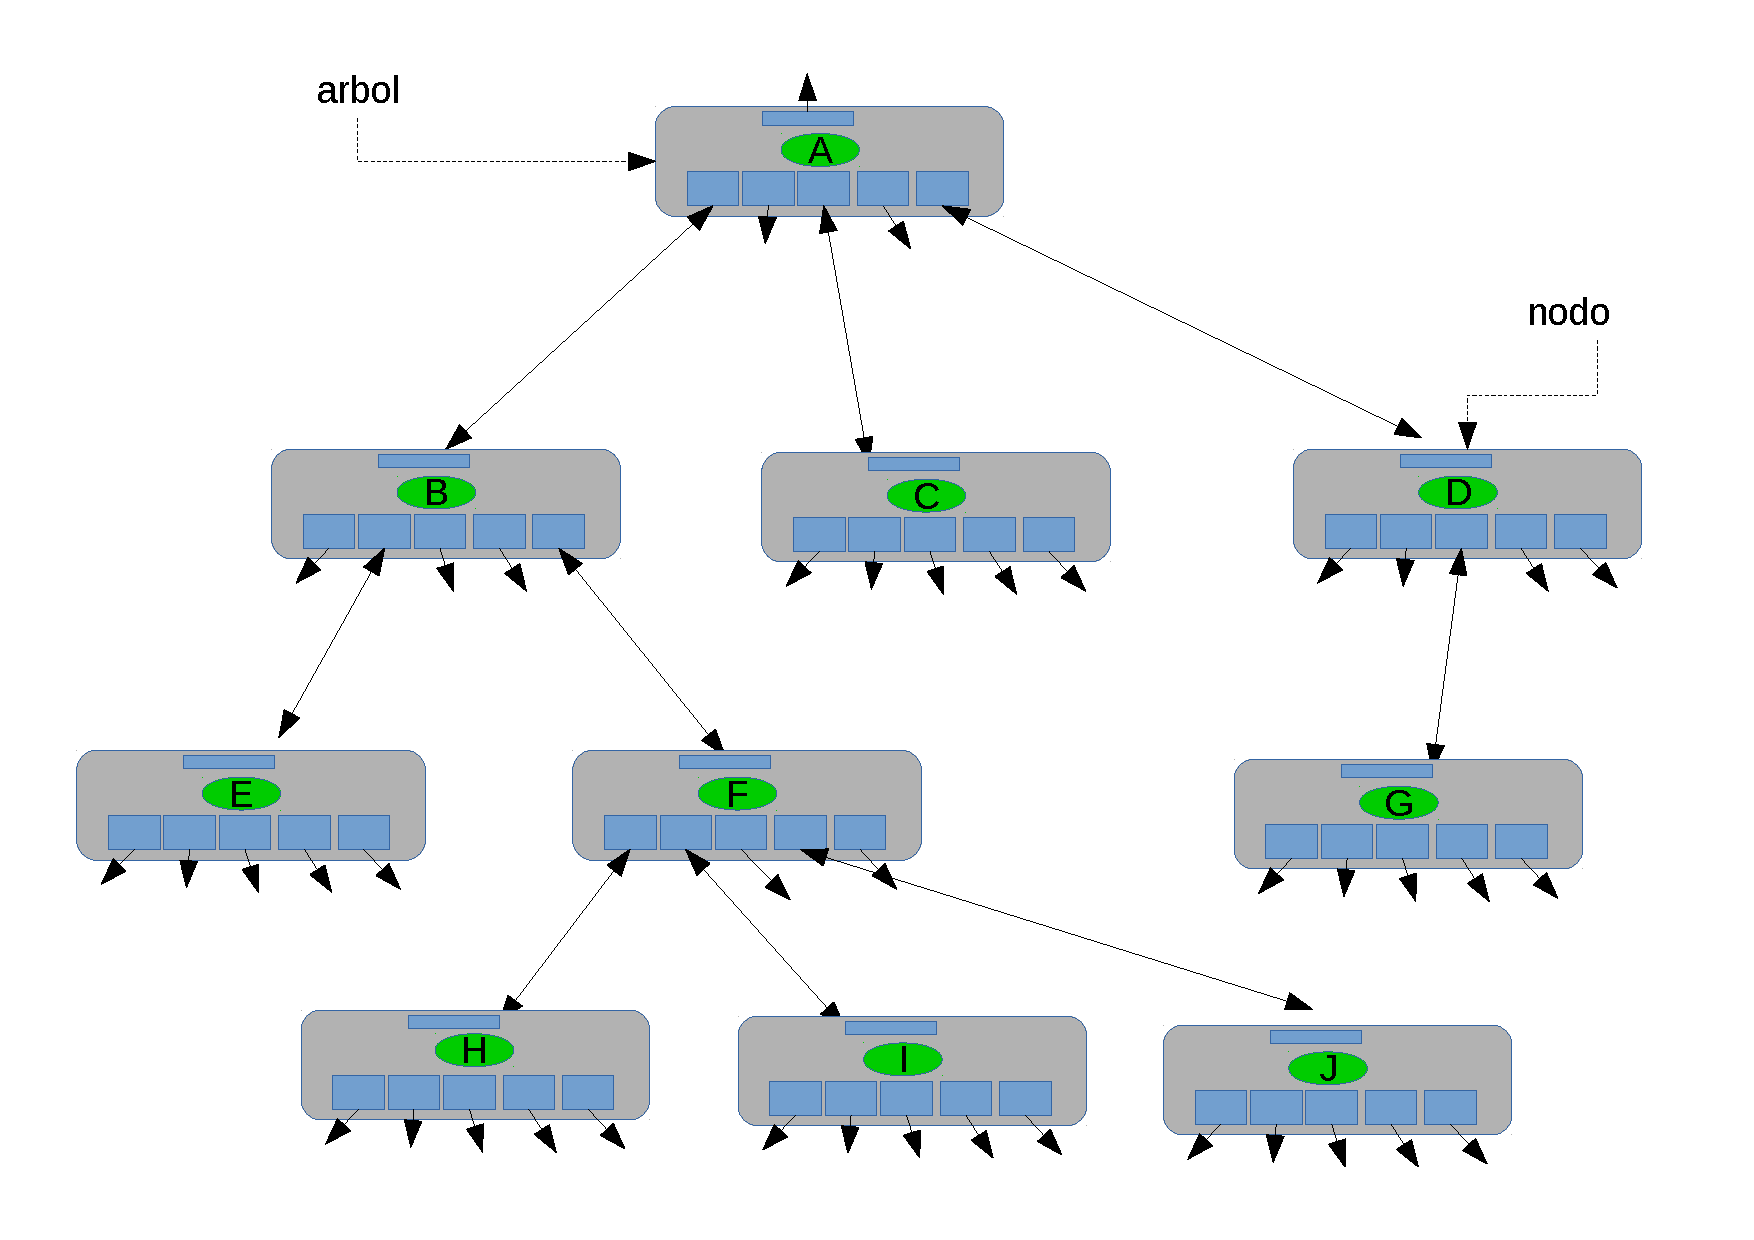
\includegraphics[width=10cm]{ktree_ejemplo}
\caption{Ejemplo de ktree}
\end{DoxyImage}



\begin{DoxyCode}
\hyperlink{classktree}{ktree<char,5>} arbol;
\hyperlink{classktree_1_1node}{ktree<char,5>::node} n, nodo;
n = arbol.\hyperlink{classktree_a2d252651d05d9a107c009fcfdfc91df4}{root}();
cout << *n \textcolor{comment}{// Nos imprime A}
nodo = n.\hyperlink{classktree_1_1node_adcb69c2caed252b51d400f4237c1f472}{k\_child}(4); \textcolor{comment}{// <- Apunta al nodo con etiqueta D}

\textcolor{keywordflow}{for} (\hyperlink{classktree_1_1node_1_1child__iterator}{ktree<char,5>::node::child\_iterator} ith : n)
  cout<< *(*ith) << endl; \textcolor{comment}{// <--  Imprime los hijos no nulos de n, esto es B,C,D}
                              \textcolor{comment}{//  *ith es el nodo hijo, *(*ith) es la etiqueta que hay dentro de dicho
       nodo.}
\end{DoxyCode}


Con el guión se entrega un código que ilustra el uso de ktree para distintos problemas (fichero {\ttfamily \hyperlink{ejemploKtree_8cpp}{ejemplo\+Ktree.\+cpp}}), como por ejemplo recorridos, cálculo de la altura de un ktree, inserción en un árbol binario de búsqueda representado mediante un ktree$<$int,2$>$, etc.

Este código, una vez compilado, debe ejecutarse desde la carpeta {\ttfamily bin}\+:


\begin{DoxyCode}
cd bin 
./ejemploKtree 
\end{DoxyCode}
\hypertarget{index_implem}{}\subsubsection{Implementación}\label{index_implem}
Puesto que conocemos el número máximo de hijos de un nodo, fijo en todo momento, podemos acceder a ellos considerando un acceso aleatorio. Esto es consultar el hijo j-\/ésimo en orden constante. Para ello, se implementa un nodo usando la siguiente estructura,


\begin{DoxyCode}
\textcolor{keyword}{struct }celdaArbol \{
  T etiqueta;
  celdaArbol * padre;
  celdaArbol * hijos[K];
\};
\end{DoxyCode}


donde \begin{DoxyItemize}
\item etiqueta representa a la etiqueta almacenada en el nodo \item padre es un puntero a la celda\+Arbol que contiene al padre de dicho nodo \item hijos es un array de tamaño fijo, K, donde en cada posición almacenamos un puntero al hijo j-\/ésimo (0$<$=j$<$K) del nodo en el árbol\end{DoxyItemize}
Considerando esta información un árbol ktree se implementará como un puntero a la celda que contiene el nodo raíz del mismo.


\begin{DoxyCode}
\textcolor{keyword}{template} <\textcolor{keyword}{typename} T, \textcolor{keywordtype}{int} K> 
\textcolor{keyword}{class }\hyperlink{classktree}{ktree} \{
  \textcolor{keyword}{public}:
   \hyperlink{classktree_a70c8511d0c0fc199f341065fab0aa0ad}{ktree}();
   ....
  \textcolor{keyword}{private}:
    celdaArbol * laraiz;
\};
\end{DoxyCode}


Como hemos comentado el T\+DA ktree contiene los siguientes tipos definidos

\begin{DoxyItemize}
\item ktree$<$\+T,\+K$>$\+::node -\/$>$ Representa un nodo del árbol \item ktree$<$T;K$>$\+::const\+\_\+node -\/$>$ Representa un nodo constante (no podemos modificar su contenido) en el árbol\end{DoxyItemize}
Donde para cada nodo (node o const\+\_\+node), su representación interna no será mas que un puntero a la celda del árbol a la que apunta, diferenciándose en el tipo de operaciones (especificación) que permiten realizar sobre el mismo (ver documentación asociada).

Si consideramos los iteradores, esto es,

\begin{DoxyItemize}
\item \hyperlink{classktree_1_1node_afa2e7c16e38c1a4a062930d167b02a7f}{ktree$<$\+T,\+K$>$\+::node\+::child\+\_\+iterator} -\/$>$ Iterador sobre los hijos no nulos de un nodo \item \hyperlink{classktree_1_1const__node_afa2e7c16e38c1a4a062930d167b02a7f}{ktree$<$\+T,\+K$>$\+::const\+\_\+node\+::child\+\_\+iterator} -\/$>$ Iterador sobre los hijos no nulos de un nodo constante\end{DoxyItemize}
Ambos iteradores tienen una representación un poco más compleja, al considerar tanto el nodo sobre el que queremos iterar como el hijo en el que ubica en este momento.

La siguiente imagen ilustra la representación interna del ktree.

 
\begin{DoxyImage}
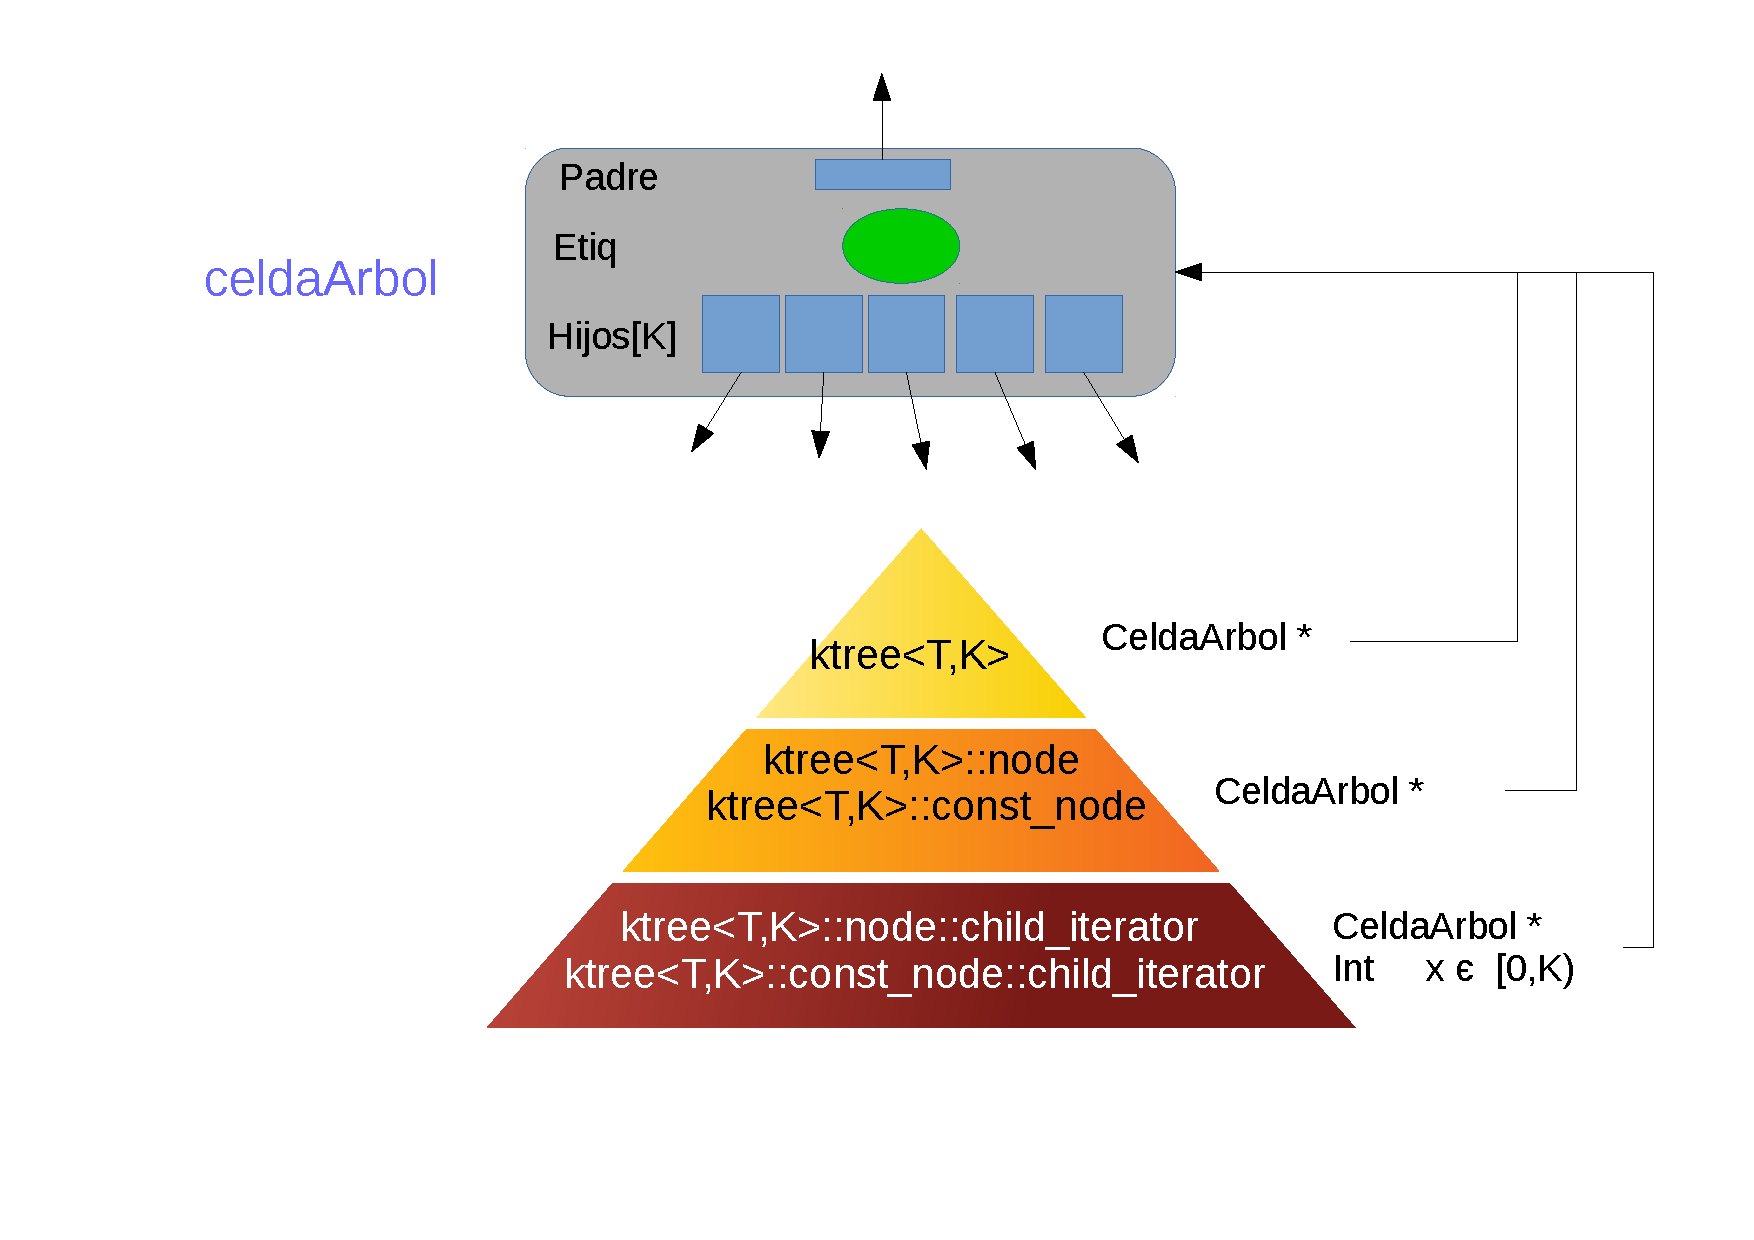
\includegraphics[width=10cm]{ktree_estructura}
\caption{Atributos de la clase ktree}
\end{DoxyImage}
\hypertarget{index_ktreegen}{}\subsection{Representando un Nmer como un ktree}\label{index_ktreegen}
\hypertarget{index_rep}{}\subsubsection{Representación}\label{index_rep}
Podemos representar todos los \hyperlink{classNmer}{Nmer} hasta una determinada longitud mediante un ktree. Para ello, en cada nodo se almacenará un char que representa a una base (A,G,C,T), excepto el nodo raíz que almacena un char nulo, por ejemplo \textquotesingle{}-\/\textquotesingle{}.

El camino que existe desde la raíz del ktree hasta un nodo n en el nivel l codificará una subsecuencia de bases consecutivas en la cadena de tamaño l. Por ejemplo, supongamos la cadena \char`\"{}\+A\+T\+A\+C\+A\+T\+C\+A\+T\+T\+G\+T\+G\+G\char`\"{}. Las distintas subsecuencias (de tamaños 1 a 3) que nos pueden aparecer son\+:

\begin{DoxyItemize}
\item Tamaño 1\+: A; G; C; T \item Tamaño 2\+: AC; AT; GG; GT; CA; TA; TG; TC; TT \item Tamaño 3\+: A\+CA; A\+TA; A\+TC; A\+TT; G\+TG; C\+AT; T\+AC; T\+GG; T\+GT; T\+CA; T\+TG\end{DoxyItemize}
Por tanto, cada nodo del árbol tendrá como máximo 4 descendientes director (hijos) que representan las posibles bases que pueden aparecer en la cadena para formar las subsecuencias de tamaño l+1, asociando cada uno a una base distinta de la siguiente forma

\begin{DoxyItemize}
\item A -\/$>$ hijo 0\end{DoxyItemize}
\begin{DoxyItemize}
\item G -\/$>$ hijo 1\end{DoxyItemize}
\begin{DoxyItemize}
\item C-\/$>$ hijo 2\end{DoxyItemize}
\begin{DoxyItemize}
\item T-\/$>$ hijo 3\end{DoxyItemize}
No olvidemos que, además de identificar las subsecuencias, estamos interesados el contar el número de veces que se repita cada una de ellas en la cadena. Para ello, es suficiente con incluir también en cada nodo del árbol un valor entero que codifique dicha información. Así, la clase \hyperlink{classNmer}{Nmer} se puede representar como se indica\+:


\begin{DoxyCode}
\textcolor{keyword}{class }\hyperlink{classNmer}{Nmer} \{
  \textcolor{keyword}{public}:
    \hyperlink{classNmer_ac2a651dd05b03e716b877c26386d772e}{Nmer}();
    ....
  \textcolor{keyword}{private}:
    \hyperlink{classktree}{ktree<pair<char,int>},4> el\_Nmer; \textcolor{comment}{// subsecuencias }
    \textcolor{keywordtype}{int} max\_long; \textcolor{comment}{// Mayor longitud de la cadena representada, esto es, el nivel máximo del árbol}
  

\};
\end{DoxyCode}


La siguiente figura muestra un subconjunto del árbol para una longitud de subcadena máxima de 3 (max\+\_\+long = 3) que se obtiene cunado consideramos la cadena \char`\"{}\+A\+T\+A\+C\+A\+T\+C\+A\+T\+T\+G\+T\+G\+G\char`\"{}, la lista todas las posibles subcadenas (junto a su frecuencia es\+: A 4; AC 1; A\+CA 1; AT 3; A\+TA 1; A\+TC 1; A\+TT 1; C 2; CA 2; C\+AT 2; G 5; GG 2; GT 1; G\+TG 1; T 5; TA 1; T\+AC 1; TC 1; T\+CA 1; TG 2; T\+GG 1; T\+GT 1; TT 1; T\+TG 1).

 
\begin{DoxyImage}
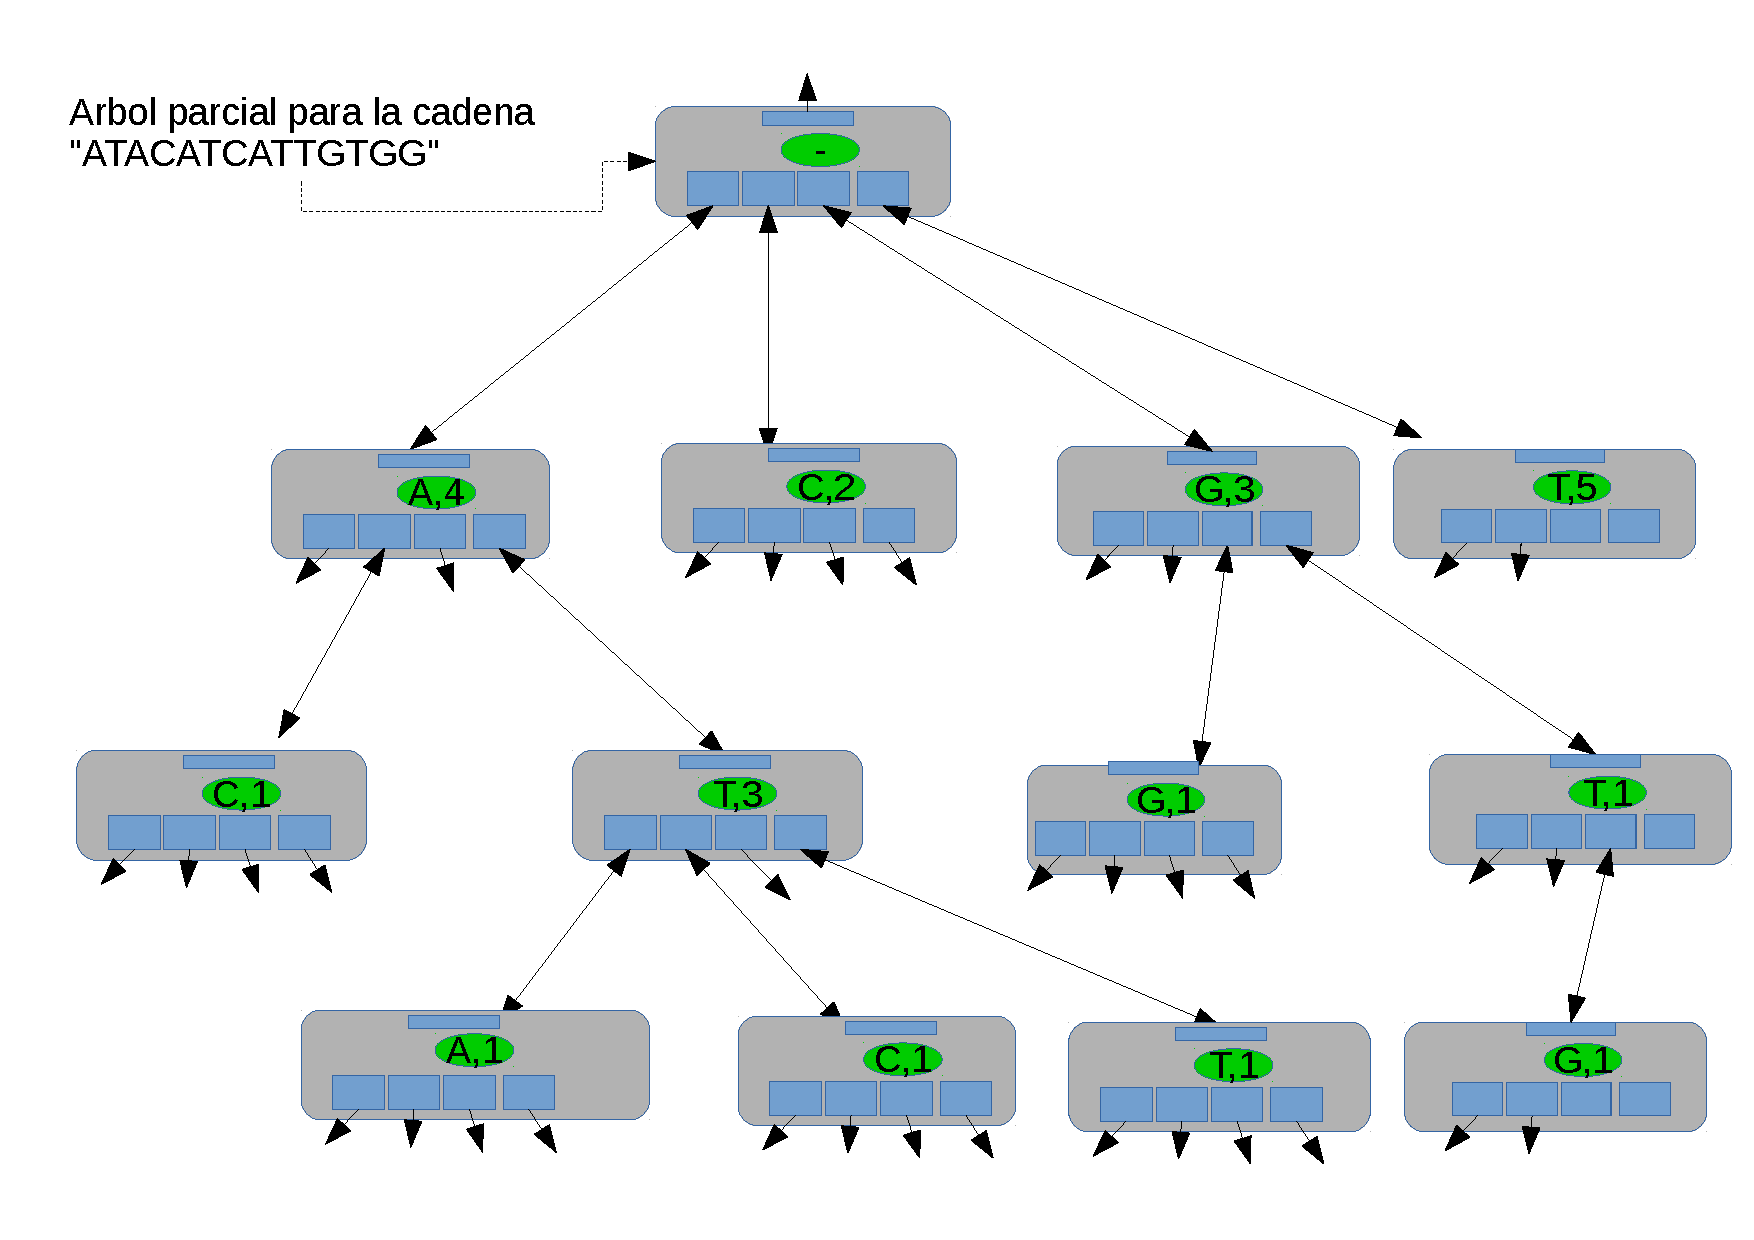
\includegraphics[width=10cm]{ktree_cadena}
\caption{Cadena de A\+DN $<$A\+T\+A\+C\+A\+T\+C\+A\+T\+T\+G\+T\+GG$>$ representada como un ktree}
\end{DoxyImage}
\hypertarget{index_otrosMetodos}{}\subsection{¿\+Cómo implementar algunos de los métodos en Nmer?}\label{index_otrosMetodos}
En esta sección presentaremos con mas detalle el comportamiento de algunos de los métodos de la clase \hyperlink{classNmer}{Nmer} que hay que implementar. Estos métodos permiten abordar distintos problemas de interés en genética computacional. Recordemos que son los métodos\+:


\begin{DoxyCode}
\textcolor{keyword}{class }\hyperlink{classNmer}{Nmer} \{
  ...

  \textcolor{keyword}{public}:

   \textcolor{keywordtype}{void} \hyperlink{classNmer_a4c29aa3845d91b09f8e0bc3517ca4ec6}{sequenceADN}(\textcolor{keywordtype}{unsigned} \textcolor{keywordtype}{int} tama, \textcolor{keyword}{const} \textcolor{keywordtype}{string} & adn);  \textcolor{comment}{// Construir Nme a partir de cadena
       de ADN}

   \textcolor{keywordtype}{bool} \hyperlink{classNmer_a418c016bb6e04d2f699ddb694ee0221f}{loadSerialized}(\textcolor{keyword}{const} \textcolor{keywordtype}{string} nombre\_fichero); \textcolor{comment}{// Leer fichero serializado que
       representa a un Nmer }

   set<pair<string,int>,\hyperlink{classOrdenCre}{OrdenCre} > \hyperlink{classNmer_a8120d82bd305662b814bdcdb30698989}{rareNmer}(\textcolor{keywordtype}{int} threshold); \textcolor{comment}{// devuelve la lista de todas
       las subcadenas (no prefijo) que  aparecen menos de threshold veces en el Nmer ordenadas en orden creciente de
       frecuencia}

   set<pair<string,int>,ordenDecre > \hyperlink{classNmer_aabaa2a3f2761170b5cbee0e822805de8}{commonNmer}(\textcolor{keywordtype}{int} threshold); \textcolor{comment}{// Devuelve la lista de las
       cadenas de longitud mayor posible (no prefijo)  que aparecen más de threshold veces en el Nmer, ordenadas en
       orden decreciente de frecuencia}
  
   set<pair<string,int>, ordenCrec > \hyperlink{classNmer_a97de70ffe49a0457e87ed249251b9c14}{level}(\textcolor{keywordtype}{int} l); \textcolor{comment}{// Devuelve el conjunto de Nmers de longitud exacta
       l.}

   \textcolor{keywordtype}{float}  \hyperlink{classNmer_a8df2f2f355423b02413e5e29dc5639e8}{Distance}(\textcolor{keyword}{const} \hyperlink{classNmer}{Nmer} & x);  \textcolor{comment}{// Distancia entre  dos Nmer}

  ...
\}
\end{DoxyCode}


El alumno podrá dotar al tipo de dato de otros métodos que considere necesarios para la correcta realización de la práctica, pero debe respetar escrupulosamente la cabecera de los métodos detallados anteriormente.\hypertarget{index_crear}{}\subsubsection{Método 1 -\/$>$  Nmer\+::sequence\+A\+D\+N(tama, adn) \+: Obteniendo los Nmers a partir de una cadena de A\+DN}\label{index_crear}
El primer problema que nos tendremos que plantear a la hora de solucionar la práctica es el poder construir el ktree que representa los distintos Nmers. Como ya hemos comentado, utilizaremos un ktree con valor k=4, donde en cada nodo almacenamos no sólo la base, sino también su frecuencia dentro de la cadena de A\+DN. En cierto sentido, el nodo en el nivel i-\/ésimo representa un \hyperlink{classNmer}{Nmer} de longitud i (dicho \hyperlink{classNmer}{Nmer} se obtiene al considerar, en orden inverso, el camino que hay desde dicho nodo a la raíz del árbol). Recordad que en cada nodo almacenamos no sólo la base, sino también el contador que nos indica las ocurrencias del \hyperlink{classNmer}{Nmer} que representa el nodo en la secuencia de A\+DN.

En esta sección trataremos de ilustrar de forma detallada cómo podemos construir a partir de la secuencia el árbol de Nmers, esto es, nuestro ktree. Para ello consideraremos dos métodos, el primero, sequence\+A\+DN, que se encarga de recorrer la cadena de A\+DN para extraer una a una todas las subcadenas de longitud tama de que se extraen los distintos Nmers a insertar, y el segundo es un método privado, insertar\+\_\+cadena, que dada una subsecuencia de tamaño tama se encarga de insertar los \char`\"{}tama\char`\"{} Nmers, subsecuencias que empiezan en cadena\mbox{[}0\mbox{]} y con longitud 1 hata cadena.\+size(), en el árbol.

Por ejemplo, si adn = \char`\"{}\+A\+T\+A\+C\+A\+T\+C\+A\+T\+T\+G\+T\+G\+G\char`\"{} y tama es 6, sequence\+A\+DN extraería las subsecuencias


\begin{DoxyItemize}
\item \char`\"{}\+A\+T\+A\+C\+A\+T\char`\"{}
\item \char`\"{}\+T\+A\+C\+A\+T\+C\char`\"{}
\item \char`\"{}\+A\+C\+A\+T\+C\+A\char`\"{}
\item \char`\"{}\+C\+A\+T\+C\+A\+T\char`\"{}
\item ...
\end{DoxyItemize}

En pseudo-\/código, sequence\+A\+DN podría implementarse como sigue


\begin{DoxyCode}
\textcolor{keywordtype}{void} \hyperlink{classNmer_a4c29aa3845d91b09f8e0bc3517ca4ec6}{Nmer::sequenceADN}(\textcolor{keywordtype}{unsigned} \textcolor{keywordtype}{int} tama, \textcolor{keyword}{const} \textcolor{keywordtype}{string} & adn)\{

Inicializamos el árbol poniendo la  etiqueta (\textcolor{charliteral}{'-'},0) en el nodo raíz 

    Para cada uno de las posiciones, i,  de la cadena \{
       Obtenemos un substring de tamaño tama que empiece en adn[i];
       insertar\_cadena(subcadena);
     \}
\}
\end{DoxyCode}


Si nos centramos en cada una de las cadenas, insertar\+\_\+cadena permite considerar los Nmers que empiezan en cadena.\+begin(). Por ejemplo, considerando un tamaño hasta 6, los distintos Nmers para \char`\"{}\+A\+T\+A\+C\+A\+T\char`\"{} son\+:


\begin{DoxyEnumerate}
\item \char`\"{}\+A\char`\"{}
\item \char`\"{}\+A\+T\char`\"{}
\item \char`\"{}\+A\+T\+A\char`\"{}
\item \char`\"{}\+A\+T\+A\+C\char`\"{}
\item \char`\"{}\+A\+T\+A\+C\+A\char`\"{}
\item \char`\"{}\+A\+T\+A\+C\+A\+T\char`\"{}
\end{DoxyEnumerate}

El esquema del algoritmo insertar\+\_\+cadena es el siguiente\+: avanzar por la cadena a la vez que descendemos por el árbol para actualizar los valores del \hyperlink{classNmer}{Nmer} que representa, como indica el siguiente pseudo-\/código\+:


\begin{DoxyCode}
\textcolor{keywordtype}{void} insertar\_cadena(\textcolor{keyword}{const} \textcolor{keywordtype}{string} & cadena)\{

posicionamos un nodo, n\_act, en la raiz del arbol.

 \textcolor{comment}{//Este nodo n lo utilizamos para descender por el arbol}
\textcolor{comment}{// cadena[i] nos indica el índice del nodo en el  nivel i+1;}
\textcolor{comment}{// A -> hijo 0; G -> hijo 1; C-> hijo 2; T-> hijo 3}

 Para cada uno de los caracteres, i, de la cadena \{
    cadena[i] nos indica el índice del nodo en el  nivel i+1;
    \textcolor{comment}{// si cadena[i] es : A -> hijo 0; G -> hijo 1; C-> hijo 2; T-> hijo 3}
    si n\_act tiene hijo en la posición dada por cadena[i] \{ \textcolor{comment}{// Ya esta insertado el nodo}
      incrementamos el contador en 1;
    \}
    en caso contrario \{ \textcolor{comment}{//  No esta insertado el nodo}
        insertamos el nuevo nodo en dicha posición con etiqueda cadena[i] y su contador a 1;
    \}
   descendemos en el árbol, haciendo que n\_act sea el nodo que representa cadena[i], esto es bajamos al 
      hijo correspondiente;
 \}

\}
\end{DoxyCode}


Para finalizar, os entregamos el código que nos recorre el ktree en preorden, donde por ejemplo la acción sobre el hijo podría ser obtener el \hyperlink{classNmer}{Nmer} que representa el nodo. En este algoritmo, n será el nodo a partir del cual queremos realizar el recorrido en preorden\+:


\begin{DoxyCode}
\textcolor{keywordtype}{void} \hyperlink{ejemploKtree_8cpp_a7ae38f4399966752d1ca1d20d24b63ac}{recorrido\_preorden}( \hyperlink{classktree}{ktree}<pair<char,int>,4>::node  n)\{

\textcolor{keywordflow}{if} (!n.null())\{
   < accion sobre el nodo n >
   \textcolor{keywordflow}{for} ( \hyperlink{classktree_1_1node}{ktree<base,4>::node} hijo : n)
     \hyperlink{ejemploKtree_8cpp_a7ae38f4399966752d1ca1d20d24b63ac}{recorrido\_preorden}(hijo);
  \}
\}
\end{DoxyCode}
\hypertarget{index_load}{}\subsubsection{Método 2 -\/$>$  Nmer\+::load\+Serialized(nombre)}\label{index_load}
Por si el alumno tiene problema en la construcción del \hyperlink{classNmer}{Nmer}, se entrega este método ya implementado que a partir de un fichero serializado, con extensión .srl, y nos reconstruye el ktree que lo generó. Con la práctica se entregan algunos ejemplos de ficheros serializdos que podrán ser utilizados por el alumno para obtener distintos Nmers válidos, como por ejemplo cadena\+Simple.\+srl, cadenabos\+Taurus.\+srl o cadenamus\+Musculus.\+srl.

Por tanto podremos utilizar este método para ir avanzando en la implementación de los otros métodos de la clase aun cuando no tengamos implementado el método que a partir de una cadena extree los Nmers, esto es, sequence\+A\+DN.

Un ejemplo de cómo poder utilizar este método lo lo podemos encontrar en el fichero \hyperlink{ejemploKtree_8cpp}{ejemplo\+Ktree.\+cpp}\+:


\begin{DoxyCode}
\hyperlink{classNmer}{Nmer} prueba;
prueba.\hyperlink{classNmer_a418c016bb6e04d2f699ddb694ee0221f}{loadSerialized}(\textcolor{stringliteral}{"cadenaSimple.srl"});
cout << prueba.\hyperlink{classNmer_a60e2335600c01ee39e865790015818f0}{length}(); \textcolor{comment}{// devuelve 3}
cout << prueba.\hyperlink{classNmer_accdea65838fcd53c48a2d05f6809643f}{size}(); \textcolor{comment}{// devuelve 24}
prueba.\hyperlink{classNmer_a1ce1c0cb174d94685c7234f58f9dc119}{list\_Nmer}();  \textcolor{comment}{// Listaria todos los Nmers (desde longitud 1 hasta longitud prueba.length()}
\end{DoxyCode}


Sólo a nivel informativo, indicar que para poder reconvertir el fichero serializado necesitamos de un functor que nos permita transformar un string del tipo \char`\"{}\+A 45\char`\"{} o \char`\"{}x -\/1\char`\"{}, donde el primer elemento de la cadena es un char y el segundo un entero, en un objeto de tipo pair$<$char,int$>$. Dicho functor, se encuentra dentro de la parte privada de la clase \hyperlink{classNmer}{Nmer} con el nombre String2\+Base.

El código para load\+Serialized (ya incluido en el {\ttfamily \hyperlink{Nmer_8cpp}{Nmer.\+cpp}}) es el siguiente\+:


\begin{DoxyCode}
\textcolor{keywordtype}{bool} \hyperlink{classNmer_a418c016bb6e04d2f699ddb694ee0221f}{Nmer::loadSerialized}(\textcolor{keyword}{const} \textcolor{keywordtype}{string} & fichero) \{
 \textcolor{keywordtype}{string} cadena;
 ifstream fe;
 pair<char,int> nulo(\textcolor{charliteral}{'x'},-1);
 Nmer::String2Base stb;
 
 fe.open(fichero.c\_str(), ifstream::in);
   \textcolor{keywordflow}{if} (fe.fail())\{
     cerr << \textcolor{stringliteral}{"Error al abrir el fichero "} << fichero << endl;
   \} 
   \textcolor{keywordflow}{else} \{
    \textcolor{comment}{//leo la cabecera del fichero (líneas que comienzan con #)}
    \textcolor{keywordflow}{do}\{ 
      getline(fe,cadena,\textcolor{charliteral}{'\(\backslash\)n'}); 
    \} \textcolor{keywordflow}{while} (cadena.find(\textcolor{stringliteral}{"#"})==0 && !fe.eof());
    \textcolor{comment}{// leemos Nmer\_length}
     max\_long = std::stoi(cadena);
     \textcolor{comment}{// leemos cadena serializada}
    getline(fe,cadena,\textcolor{charliteral}{'\(\backslash\)n'});
    el\_Nmer.\hyperlink{classktree_a66d27ffb43b3c790370b45c0a8309534}{deserialize}(cadena,nulo,\textcolor{charliteral}{';'},stb); 
    fe.close();
    \textcolor{keywordflow}{return} \textcolor{keyword}{true};
  \} \textcolor{comment}{// else}
  fe.close();
  \textcolor{keywordflow}{return} \textcolor{keyword}{false};
 \}
\end{DoxyCode}
\hypertarget{index_rare}{}\subsubsection{Método 3 -\/$>$ set$<$pair$<$string,int$>$,\+Orden\+Cre $>$ Nmer\+::rare\+Nmer(threshold)}\label{index_rare}
Este método devuelve la lista de todas las subcadenas (no prefijo) que aparecen un número menor o igual a threshold veces en el \hyperlink{classNmer}{Nmer}. Estas cadenas se almacenarán en el primer campo del par, mientras que en el segundo dispondremos de la frecuencia de aparición en la cadena de A\+DN de dicho \hyperlink{classNmer}{Nmer}. EL conjunto deberá estar ordenado en orden creciente de frecuencia, esto es las cadenas (por ejemplo, esto se utiliza para buscar peculiaridades en la secuencia de A\+DN).

$<$bf$>$¿\+Qué es una cadena prefijo?\+:$<$/bf$>$ decimos que una cadena, x, es prefijo de otra, y, si x está completamente incluida en y empezando desde el principio. Por ejemplo x=\char`\"{}abcde\char`\"{} es prefijo de \char`\"{}abcdefg\char`\"{} pero no lo es de \char`\"{}sabcdefg\char`\"{}.

Por tanto, si realizamos una llamada al método rare\+Nmer(4), esto es threshold es 4, y encontramos que el \hyperlink{classNmer}{Nmer} \char`\"{}\+A\+C\char`\"{} aparece 5 veces, \hyperlink{classNmer}{Nmer} \char`\"{}\+A\+C\+G\char`\"{} aparece 4 veces, el \hyperlink{classNmer}{Nmer} \char`\"{}\+A\+C\+G\+G\char`\"{} aparece 2 y \char`\"{}\+A\+C\+G\+T\char`\"{} aparece 1, como salida sólo nos debería devolver \char`\"{}\+A\+C\+G\+G\char`\"{} y \char`\"{}\+A\+C\+G\+T\char`\"{}, pues \char`\"{}\+A\+C\+G\char`\"{}, aun teniendo una frecuencia menor o igual que el threshold 4, es prefijo de al menos otra cadena de longitud mayor.\hypertarget{index_common}{}\subsubsection{Método 4 -\/$>$  set$<$pair$<$string,int$>$,orden\+Decre $>$ common\+Nmer(threshold)}\label{index_common}
Devuelve la lista de las cadenas de longitud mayor posible (sin ser prefijo) que aparecen un número de veces mayor que de threshold veces en el \hyperlink{classNmer}{Nmer}, ordenadas en orden decreciente de frecuencia (se utiliza para buscar repeticiones mas comunes, por ejemplo cuando tratamos de comprimir una cadena de A\+DN). Al igual que antes, el conjunto de cadenas deberá estar ordenado, pero en este caso en orden decreciente, esto es, aparecen primero las maś frecuentes

Por ejemplo, si consideramos que un \hyperlink{classNmer}{Nmer} contiene a \char`\"{}\+A\+C\char`\"{} que aparece 5 veces, a \char`\"{}\+A\+T\char`\"{} que aparece 5 veces, a \char`\"{}\+A\+C\+G\char`\"{} que aparece 4 veces, \char`\"{}\+A\+C\+T\char`\"{} que aparece 4 veces, \char`\"{}\+A\+T\+G\char`\"{} que aparece 3 veces \char`\"{}\+A\+C\+G\+G\char`\"{} que aparece 2 y \char`\"{}\+A\+C\+G\+T\char`\"{} que aparece 1, una llamada a {\ttfamily common\+Nmer(3)} dará como salida \char`\"{}\+A\+T\char`\"{}, \char`\"{}\+A\+C\+G\char`\"{} y \char`\"{}\+A\+C\+T\char`\"{}. En este caso \char`\"{}\+A\+C\char`\"{}, aun teniendo una frecuencia mayor que el threshold 4, es prefijo de al menos otra cadena de longitud mayor.\hypertarget{index_level}{}\subsubsection{Método 5 -\/$>$ set$<$pair$<$string,int$>$, orden\+Crec $>$ level(l);}\label{index_level}
Este método nos devuelve únicamente los Nmers de longitud l, ordenados en orden creciente de frecuencia.

Por ejemplo, si consideramos que un \hyperlink{classNmer}{Nmer} contiene a \char`\"{}\+A\+C\char`\"{} que aparece 5 veces, a \char`\"{}\+A\+T\char`\"{} que aparece 5 veces, a \char`\"{}\+A\+C\+G\char`\"{} que aparece 4 veces, \char`\"{}\+A\+C\+T\char`\"{} que aparece 4 veces, \char`\"{}\+A\+T\+G\char`\"{} que aparece 3 veces \char`\"{}\+A\+C\+G\+G\char`\"{} que aparece 2 y \char`\"{}\+A\+C\+G\+T\char`\"{} que aparece 1, una llamada a {\ttfamily level(3)} dará como salida \char`\"{}\+A\+T\+G\char`\"{}, \char`\"{}\+A\+C\+G\char`\"{} y \char`\"{}\+A\+C\+T\char`\"{} y , con frecuencia 3, 4 y 4, respectivamente.\hypertarget{index_problemaBiologia}{}\subsubsection{Método 6 -\/$>$ float Distance(\+Nmer) \+: Aplicación del T\+D\+A Nmer a la caracterización del genoma de distintas especies.}\label{index_problemaBiologia}
Una vez programado el T\+DA \hyperlink{classNmer}{Nmer} descrito en las secciones anteriores, proponemos que el estudiante aplique este T\+DA a un problema real\+: la identificación de especies en base a los Nmers de una secuencia de A\+DN. Para ello, se proporciona al estudiante extractos reales de longitud 10.\+000 de cadenas de A\+DN del genoma de 10 especies animales (ficheros {\ttfamily datos/1.\+txt}, {\ttfamily datos/2.\+txt}, ..., {\ttfamily datos/10.\+txt}). El estudiante debe construir un objeto \hyperlink{classNmer}{Nmer} para representar cada una de estas 10 secuencias de A\+DN. Una vez creados los Nmers, el estudiante deberá implementar una métrica para medir la distancia entre estos Nmers para identificar cuáles son las cadenas más parecidas entre sí. El fichero {\ttfamily datos/genomas disponibles.\+txt} muestra a qué especie corresponde cada cadena de A\+DN. Si los métodos están bien implementados y el tamaño de N es suficientemente elevado (recomendamos probar valores de N$>$=10), los resultados deben ir acordes a la distancia evolutiva entre las especies \mbox{[}3\mbox{]}\+: por ejemplo, las cadenas humanas serán más parecidas entre sí o a las de ratón que a las de gusano. En cualquier caso, nuestros resultados pueden fluctuar dado que estamos considerando extractos de longitud reducida (10.\+000 bases es un tamaño reducido dado el tamaño total de los genomas considerados).\hypertarget{index_dist}{}\paragraph{Cálculo de la Distancia}\label{index_dist}
En esta sección detallaremos cómo se calcula la distancia entre dos Nmers. Para ello consideremos el siguiente ejemplo donde trataremos de buscar la distancia entre los Nmers, nmX e nmY, asociados a considerar dos cadenas de A\+DN, adnX y adnY, respectivamente. Ilustraremos cómo sería al proceso para calcular 
\begin{DoxyCode}
nmX.distance(nmY);
\end{DoxyCode}


En nuestro caso asumiremos que ambos datos tienen como longitud máxima 2 (presentados como una secuencia de pares \hyperlink{classNmer}{Nmer}=frecuencia).

\begin{DoxyItemize}
\item nmX\+: (A=690) (G=1019) (C=818) (T=694) (AA=199) (AG=282) (AC=99) (AT=109) (GA=257) (GG=372) (GC=231) (GT=159) (CA=153) (CG=162) (CC=284) (CT=219) (TA=81) (TG=202) (TC=204) (TT=207) \item nmY\+: (A=985) (G=1202) (C=1262) (T=991) (AA=270) (AG=341) (AC=219) (AT=155) (GA=261) (GG=423) (GC=300) (GT=217) (CA=349) (CC=456) (CT=386) (TG=367) (TC=286) (TT=233)\end{DoxyItemize}
El primer paso consiste en ordenar los distintos Nmers de forma que los más frecuentes ocupen las primeras posiciones en el orden. Una alternativa para abordar este problema es utilizar un contenedor asociativo, tipo set, que almacene cada uno de los pares pero considerando como criterio de comparación el de mayor frecuencia. Como resultado tendríamos este secuencia de elementos (\hyperlink{classNmer}{Nmer} frecuencia).

\begin{DoxyItemize}
\item nmX\+: G 1019;C 818;T 694;A 690;GG 372;CC 284;AG 282;GA 257;GC 231;CT 219;TT 207;TC 204;TG 202;AA 199;CG 162;GT 159;CA 153;AT 109;AC 99;TA 81; \item nmY\+: C 1262;G 1202;T 991;A 985;CC 456;GG 423;CT 386;TG 367;CA 349;AG 341;GC 300;TC 286;AA 270;GA 261;TT 233;AC 219;GT 217;AT 155;\end{DoxyItemize}
Iterando sobre este contenedor es fácil asociar a cada \hyperlink{classNmer}{Nmer} su posición en el ranking. Así para adnX el \hyperlink{classNmer}{Nmer} G tendrá valor 1, \hyperlink{classNmer}{Nmer} C tendrá valor 2, \hyperlink{classNmer}{Nmer} T será 3, ... Esto es,

\begin{DoxyItemize}
\item rankingX\+: G 1; C 2; T 3; A 4; GG 5; CC 6; AG 7; GA 8; GC 9; CT 10; TT 11; TC 12; TG 13; AA 14; CG 15; GT 16; CA 17; AT 18; AC 19; TA 20; \item rankingY\+: C 1; G 2; T 3; A 4; CC 5; GG 6; CT 7; TG 8; CA 9; AG 10; GC 11; TC 12; AA 13; GA 14; TT 15; AC 16; GT 17; AT 18;\end{DoxyItemize}
Una vez que tenemos este ranking podremos proceder a calcular la distancia teniendo en cuenta la distancia entre las posiciones en cada ranking. Así, por ejemplo G está a distancia 1 (diferencia entre 1 y 2), T está a distancia 0, TG está a distancia 5 (diferencia entre 13 y 8), ... y finalmente si consideramos tanto CG como TA diremos que están a distancia máxima (definida como la distancia máxima posible entre los rankings) ya que ambos Nmers no se encuentran en el rankingY.

Finalmente indicar que estas distancias (normalizadas) son acumuladas, devolviendo el promedio

El siguiente pseudo código nos permite computar dicha distancia\+: 
\begin{DoxyCode}
max <- maximo(rankingX.size(),rankingY.size());
dist <- 0;
Para cada \hyperlink{classNmer}{Nmer} n en rankingX \{
  Si (n pertenece a rankingY) \{
    posX <- la posicion de n en rankingX
    posY <- la posicion de n en rankingY;
        valor = abs(posX-posY)/max
  \} \textcolor{keywordflow}{else} valor = 1;
  dist+=valor;
 \} 
\textcolor{keywordflow}{return} dist/rankingX.\hyperlink{classNmer_accdea65838fcd53c48a2d05f6809643f}{size}() \textcolor{comment}{// calculamos el promedio, tomando  valores en [0,1]}
\end{DoxyCode}


Finalmente, indicar que la distancia, tal y como está definida no es simétrica, esto es nm\+X.\+distance(nm\+Y) != nm\+Y.\+distance(nm\+X)\hypertarget{index_entrega}{}\subsection{Entrega}\label{index_entrega}
El alumno debe empaquetar todos los archivos relacionados con el proyecto en un archivo con nombre \char`\"{}gen\+Data.\+zip\char`\"{}. Tenga en cuenta que no se incluirán ficheros objeto, ni ejecutables. Es recomendable que haga una \char`\"{}limpieza\char`\"{} para eliminar los archivos temporales o que se puedan generar a partir de los fuentes.

El alumno debe incluir un fichero con un main {\ttfamily src/ejemplo\+Nmer.\+cpp} que exhiba toda la funcionalidad programada para el T\+DA \hyperlink{classNmer}{Nmer}, incluyendo el cálculo de las distancias entre las 10 secuencias de distinta especie ({\ttfamily datos/1.\+txt, datos/2.\+txt}, etc).

El alumno ya tiene disponible un fichero Makefile para realizar la compilación. Conviene estudiar con detalle este fichero y sus distintas opciones\+:
\begin{DoxyItemize}
\item {\ttfamily make} para generar los ejecutables
\item {\ttfamily make documentacion} para generar la documentación en la carpeta {\ttfamily doc/html} y {\ttfamily doc/latex}
\item {\ttfamily make clean} para eliminar ficheros temporales y objeto.
\end{DoxyItemize}

El alumno debe actualizar este fichero para compilar los nuevos módulos generados.

Tenga en cuenta que los archivos deben estar distribuidos en directorios\+:

gen\+Data.\+zip \begin{DoxyItemize}
\item Makefile \item include -- Carpeta con ficheros de cabecera (.h) \item src --Carpeta con código fuente (.cpp) \item doc --Carpeta con Documentación \item obj -- Carpeta para código objeto (.o) \item lib -- Carpeta para bibliotecas (.a) \item bin -- Carpeta para ejecutables \item datos -- Carpeta para ficheros de datos\end{DoxyItemize}
La fecha límite de entrega es el día 25 de Enero de 2017 a las 23\+:59.\hypertarget{index_bibliografia}{}\subsection{Bibliografía}\label{index_bibliografia}
\mbox{[}1\mbox{]} k-\/mer en wikipedia\+: \href{https://en.wikipedia.org/wiki/K-mer}{\tt https\+://en.\+wikipedia.\+org/wiki/\+K-\/mer}

\mbox{[}2\mbox{]} Genomic D\+NA k-\/mer spectra\+: models and modalities. (2009) Benny Chor et al. Genome Biol. 10(10)\+: R108.

\mbox{[}3\mbox{]} \href{https://genome-euro.ucsc.edu/cgi-bin/hgGateway}{\tt https\+://genome-\/euro.\+ucsc.\+edu/cgi-\/bin/hg\+Gateway} 
\section{Lista de tareas pendientes}
\label{todo}
\hypertarget{todo}{}

\begin{DoxyRefList}
\item[\label{todo__todo000001}%
\hypertarget{todo__todo000001}{}%
Miembro \hyperlink{classNmer_a1ce1c0cb174d94685c7234f58f9dc119}{Nmer\+:\+:list\+\_\+\+Nmer} () const ]Debemos de implementar este método de forma que nos garantizemos que se imprimen todos los Nmers. 
\end{DoxyRefList}
\section{Lista de bugs}
\label{bug}
\hypertarget{bug}{}

\begin{DoxyRefList}
\item[\label{bug__bug000001}%
\hypertarget{bug__bug000001}{}%
Archivo \hyperlink{ktree_8h}{ktree.h} ]Por espeficicar
\end{DoxyRefList}
\section{Índice de clases}
\subsection{Lista de clases}
Lista de las clases, estructuras, uniones e interfaces con una breve descripción\+:\begin{DoxyCompactList}
\item\contentsline{section}{\hyperlink{classktree_1_1node_1_1child__iterator}{ktree$<$ T, K $>$\+::node\+::child\+\_\+iterator} }{\pageref{classktree_1_1node_1_1child__iterator}}{}
\item\contentsline{section}{\hyperlink{classktree_1_1const__node_1_1child__iterator}{ktree$<$ T, K $>$\+::const\+\_\+node\+::child\+\_\+iterator} }{\pageref{classktree_1_1const__node_1_1child__iterator}}{}
\item\contentsline{section}{\hyperlink{classktree_1_1const__node}{ktree$<$ T, K $>$\+::const\+\_\+node} }{\pageref{classktree_1_1const__node}}{}
\item\contentsline{section}{\hyperlink{classktree}{ktree$<$ T, K $>$} }{\pageref{classktree}}{}
\item\contentsline{section}{\hyperlink{classNmer}{Nmer} }{\pageref{classNmer}}{}
\item\contentsline{section}{\hyperlink{classktree_1_1node}{ktree$<$ T, K $>$\+::node} }{\pageref{classktree_1_1node}}{}
\item\contentsline{section}{\hyperlink{classOrdenCre}{Orden\+Cre} \\*Clase \hyperlink{classOrdenCre}{Orden\+Cre} la ordena en orden creciente por la frecuencia }{\pageref{classOrdenCre}}{}
\item\contentsline{section}{\hyperlink{classOrdenDecre}{Orden\+Decre} \\*Clase \hyperlink{classOrdenDecre}{Orden\+Decre} la ordena en orden creciente por la frecuencia }{\pageref{classOrdenDecre}}{}
\item\contentsline{section}{\hyperlink{classOrdenDecreSt}{Orden\+Decre\+St} \\*Clase \hyperlink{classOrdenDecre}{Orden\+Decre} la ordena en orden creciente por la frecuencia }{\pageref{classOrdenDecreSt}}{}
\end{DoxyCompactList}

\section{Indice de archivos}
\subsection{Lista de archivos}
Lista de todos los archivos con descripciones breves\+:\begin{DoxyCompactList}
\item\contentsline{section}{include/\hyperlink{ktree_8h}{ktree.\+h} \\*T\+DA ktree$<$\+T,\+K$>$ Representa un árbol general con nodos etiquetados con datos del tipo T. Cada nodo puede tener entre 0 y K hijos como máximo, numerados de 0 a K-\/1 }{\pageref{ktree_8h}}{}
\item\contentsline{section}{include/\hyperlink{Nmer_8h}{Nmer.\+h} \\*T\+DA \hyperlink{classNmer}{Nmer} Representa un conjunto de \hyperlink{classNmer}{Nmer} subsecuencias de tamaño 1 hasta N que se pueden obtener a partir de una cadena de A\+DN }{\pageref{Nmer_8h}}{}
\item\contentsline{section}{src/\hyperlink{ejemploKtree_8cpp}{ejemplo\+Ktree.\+cpp} }{\pageref{ejemploKtree_8cpp}}{}
\item\contentsline{section}{src/\hyperlink{Nmer_8cpp}{Nmer.\+cpp} }{\pageref{Nmer_8cpp}}{}
\end{DoxyCompactList}

\section{Documentación de las clases}
\hypertarget{classktree_1_1node_1_1child__iterator}{}\subsection{Referencia de la Clase ktree$<$ T, K $>$\+:\+:node\+:\+:child\+\_\+iterator}
\label{classktree_1_1node_1_1child__iterator}\index{ktree$<$ T, K $>$\+::node\+::child\+\_\+iterator@{ktree$<$ T, K $>$\+::node\+::child\+\_\+iterator}}


{\ttfamily \#include $<$ktree.\+h$>$}

\subsubsection*{Métodos públicos}
\begin{DoxyCompactItemize}
\item 
\hyperlink{classktree_1_1node_1_1child__iterator_aa2a88529bdbc2d1ca8d0660e5e592f6b}{child\+\_\+iterator} ()
\item 
\hyperlink{classktree_1_1node_1_1child__iterator_a7fd38409a0b9f8096903ec320a297c88}{child\+\_\+iterator} (const \hyperlink{classktree_1_1node_1_1child__iterator}{child\+\_\+iterator} \&x)
\item 
\hyperlink{classktree_1_1node}{node} \& \hyperlink{classktree_1_1node_1_1child__iterator_a1086c36826bb38f4918c9b4e813f571f}{operator$\ast$} ()
\item 
\hyperlink{classktree_1_1node_1_1child__iterator}{child\+\_\+iterator} \& \hyperlink{classktree_1_1node_1_1child__iterator_ae7c1d3c7f27cc407fcf081b752d4fc0d}{operator++} ()
\item 
\hyperlink{classktree_1_1node_1_1child__iterator}{child\+\_\+iterator} \hyperlink{classktree_1_1node_1_1child__iterator_a69b171c7e0f1b17c3582fd7021efe944}{operator++} (int)
\item 
\hyperlink{classktree_1_1node_1_1child__iterator}{child\+\_\+iterator} \& \hyperlink{classktree_1_1node_1_1child__iterator_a00140b3fc82a29b9b2e5fc93fa586d55}{operator=} (const \hyperlink{classktree_1_1node_1_1child__iterator}{child\+\_\+iterator} \&x)
\item 
bool \hyperlink{classktree_1_1node_1_1child__iterator_a22cf8c7aa9de6694626c6a12e285b9df}{operator==} (const \hyperlink{classktree_1_1node_1_1child__iterator}{child\+\_\+iterator} \&x)
\item 
bool \hyperlink{classktree_1_1node_1_1child__iterator_a8b2d218a03cf3f6df5387ee3c7511ff7}{operator!=} (const \hyperlink{classktree_1_1node_1_1child__iterator}{child\+\_\+iterator} \&x)
\end{DoxyCompactItemize}
\subsubsection*{Amigas}
\begin{DoxyCompactItemize}
\item 
class \hyperlink{classktree_1_1node_1_1child__iterator_a3700a7180235e9a28534b15d5922de12}{node}
\end{DoxyCompactItemize}


\subsubsection{Descripción detallada}
\subsubsection*{template$<$typename T, int K = 2$>$\\*
class ktree$<$ T, K $>$\+::node\+::child\+\_\+iterator}



Definición en la línea 424 del archivo ktree.\+h.



\subsubsection{Documentación del constructor y destructor}
\index{ktree\+::node\+::child\+\_\+iterator@{ktree\+::node\+::child\+\_\+iterator}!child\+\_\+iterator@{child\+\_\+iterator}}
\index{child\+\_\+iterator@{child\+\_\+iterator}!ktree\+::node\+::child\+\_\+iterator@{ktree\+::node\+::child\+\_\+iterator}}
\paragraph[{\texorpdfstring{child\+\_\+iterator()}{child_iterator()}}]{\setlength{\rightskip}{0pt plus 5cm}template$<$typename T, int K = 2$>$ {\bf ktree}$<$ T, K $>$\+::node\+::child\+\_\+iterator\+::child\+\_\+iterator (
\begin{DoxyParamCaption}
{}
\end{DoxyParamCaption}
)}\hypertarget{classktree_1_1node_1_1child__iterator_aa2a88529bdbc2d1ca8d0660e5e592f6b}{}\label{classktree_1_1node_1_1child__iterator_aa2a88529bdbc2d1ca8d0660e5e592f6b}
\index{ktree\+::node\+::child\+\_\+iterator@{ktree\+::node\+::child\+\_\+iterator}!child\+\_\+iterator@{child\+\_\+iterator}}
\index{child\+\_\+iterator@{child\+\_\+iterator}!ktree\+::node\+::child\+\_\+iterator@{ktree\+::node\+::child\+\_\+iterator}}
\paragraph[{\texorpdfstring{child\+\_\+iterator(const child\+\_\+iterator \&x)}{child_iterator(const child_iterator &x)}}]{\setlength{\rightskip}{0pt plus 5cm}template$<$typename T, int K = 2$>$ {\bf ktree}$<$ T, K $>$\+::node\+::child\+\_\+iterator\+::child\+\_\+iterator (
\begin{DoxyParamCaption}
\item[{const {\bf child\+\_\+iterator} \&}]{x}
\end{DoxyParamCaption}
)}\hypertarget{classktree_1_1node_1_1child__iterator_a7fd38409a0b9f8096903ec320a297c88}{}\label{classktree_1_1node_1_1child__iterator_a7fd38409a0b9f8096903ec320a297c88}


\subsubsection{Documentación de las funciones miembro}
\index{ktree\+::node\+::child\+\_\+iterator@{ktree\+::node\+::child\+\_\+iterator}!operator"!=@{operator"!=}}
\index{operator"!=@{operator"!=}!ktree\+::node\+::child\+\_\+iterator@{ktree\+::node\+::child\+\_\+iterator}}
\paragraph[{\texorpdfstring{operator"!=(const child\+\_\+iterator \&x)}{operator!=(const child_iterator &x)}}]{\setlength{\rightskip}{0pt plus 5cm}template$<$typename T, int K = 2$>$ bool {\bf ktree}$<$ T, K $>$\+::node\+::child\+\_\+iterator\+::operator!= (
\begin{DoxyParamCaption}
\item[{const {\bf child\+\_\+iterator} \&}]{x}
\end{DoxyParamCaption}
)}\hypertarget{classktree_1_1node_1_1child__iterator_a8b2d218a03cf3f6df5387ee3c7511ff7}{}\label{classktree_1_1node_1_1child__iterator_a8b2d218a03cf3f6df5387ee3c7511ff7}
\index{ktree\+::node\+::child\+\_\+iterator@{ktree\+::node\+::child\+\_\+iterator}!operator$\ast$@{operator$\ast$}}
\index{operator$\ast$@{operator$\ast$}!ktree\+::node\+::child\+\_\+iterator@{ktree\+::node\+::child\+\_\+iterator}}
\paragraph[{\texorpdfstring{operator$\ast$()}{operator*()}}]{\setlength{\rightskip}{0pt plus 5cm}template$<$typename T, int K = 2$>$ {\bf node}\& {\bf ktree}$<$ T, K $>$\+::node\+::child\+\_\+iterator\+::operator$\ast$ (
\begin{DoxyParamCaption}
{}
\end{DoxyParamCaption}
)}\hypertarget{classktree_1_1node_1_1child__iterator_a1086c36826bb38f4918c9b4e813f571f}{}\label{classktree_1_1node_1_1child__iterator_a1086c36826bb38f4918c9b4e813f571f}
\index{ktree\+::node\+::child\+\_\+iterator@{ktree\+::node\+::child\+\_\+iterator}!operator++@{operator++}}
\index{operator++@{operator++}!ktree\+::node\+::child\+\_\+iterator@{ktree\+::node\+::child\+\_\+iterator}}
\paragraph[{\texorpdfstring{operator++()}{operator++()}}]{\setlength{\rightskip}{0pt plus 5cm}template$<$typename T, int K = 2$>$ {\bf child\+\_\+iterator}\& {\bf ktree}$<$ T, K $>$\+::node\+::child\+\_\+iterator\+::operator++ (
\begin{DoxyParamCaption}
{}
\end{DoxyParamCaption}
)}\hypertarget{classktree_1_1node_1_1child__iterator_ae7c1d3c7f27cc407fcf081b752d4fc0d}{}\label{classktree_1_1node_1_1child__iterator_ae7c1d3c7f27cc407fcf081b752d4fc0d}
\index{ktree\+::node\+::child\+\_\+iterator@{ktree\+::node\+::child\+\_\+iterator}!operator++@{operator++}}
\index{operator++@{operator++}!ktree\+::node\+::child\+\_\+iterator@{ktree\+::node\+::child\+\_\+iterator}}
\paragraph[{\texorpdfstring{operator++(int)}{operator++(int)}}]{\setlength{\rightskip}{0pt plus 5cm}template$<$typename T, int K = 2$>$ {\bf child\+\_\+iterator} {\bf ktree}$<$ T, K $>$\+::node\+::child\+\_\+iterator\+::operator++ (
\begin{DoxyParamCaption}
\item[{int}]{}
\end{DoxyParamCaption}
)}\hypertarget{classktree_1_1node_1_1child__iterator_a69b171c7e0f1b17c3582fd7021efe944}{}\label{classktree_1_1node_1_1child__iterator_a69b171c7e0f1b17c3582fd7021efe944}
\index{ktree\+::node\+::child\+\_\+iterator@{ktree\+::node\+::child\+\_\+iterator}!operator=@{operator=}}
\index{operator=@{operator=}!ktree\+::node\+::child\+\_\+iterator@{ktree\+::node\+::child\+\_\+iterator}}
\paragraph[{\texorpdfstring{operator=(const child\+\_\+iterator \&x)}{operator=(const child_iterator &x)}}]{\setlength{\rightskip}{0pt plus 5cm}template$<$typename T, int K = 2$>$ {\bf child\+\_\+iterator}\& {\bf ktree}$<$ T, K $>$\+::node\+::child\+\_\+iterator\+::operator= (
\begin{DoxyParamCaption}
\item[{const {\bf child\+\_\+iterator} \&}]{x}
\end{DoxyParamCaption}
)}\hypertarget{classktree_1_1node_1_1child__iterator_a00140b3fc82a29b9b2e5fc93fa586d55}{}\label{classktree_1_1node_1_1child__iterator_a00140b3fc82a29b9b2e5fc93fa586d55}
\index{ktree\+::node\+::child\+\_\+iterator@{ktree\+::node\+::child\+\_\+iterator}!operator==@{operator==}}
\index{operator==@{operator==}!ktree\+::node\+::child\+\_\+iterator@{ktree\+::node\+::child\+\_\+iterator}}
\paragraph[{\texorpdfstring{operator==(const child\+\_\+iterator \&x)}{operator==(const child_iterator &x)}}]{\setlength{\rightskip}{0pt plus 5cm}template$<$typename T, int K = 2$>$ bool {\bf ktree}$<$ T, K $>$\+::node\+::child\+\_\+iterator\+::operator== (
\begin{DoxyParamCaption}
\item[{const {\bf child\+\_\+iterator} \&}]{x}
\end{DoxyParamCaption}
)}\hypertarget{classktree_1_1node_1_1child__iterator_a22cf8c7aa9de6694626c6a12e285b9df}{}\label{classktree_1_1node_1_1child__iterator_a22cf8c7aa9de6694626c6a12e285b9df}


\subsubsection{Documentación de las funciones relacionadas y clases amigas}
\index{ktree\+::node\+::child\+\_\+iterator@{ktree\+::node\+::child\+\_\+iterator}!node@{node}}
\index{node@{node}!ktree\+::node\+::child\+\_\+iterator@{ktree\+::node\+::child\+\_\+iterator}}
\paragraph[{\texorpdfstring{node}{node}}]{\setlength{\rightskip}{0pt plus 5cm}template$<$typename T, int K = 2$>$ friend class {\bf node}\hspace{0.3cm}{\ttfamily [friend]}}\hypertarget{classktree_1_1node_1_1child__iterator_a3700a7180235e9a28534b15d5922de12}{}\label{classktree_1_1node_1_1child__iterator_a3700a7180235e9a28534b15d5922de12}


Definición en la línea 426 del archivo ktree.\+h.



La documentación para esta clase fue generada a partir del siguiente fichero\+:\begin{DoxyCompactItemize}
\item 
include/\hyperlink{ktree_8h}{ktree.\+h}\end{DoxyCompactItemize}

\hypertarget{classktree_1_1const__node_1_1child__iterator}{}\subsection{Referencia de la Clase ktree$<$ T, K $>$\+:\+:const\+\_\+node\+:\+:child\+\_\+iterator}
\label{classktree_1_1const__node_1_1child__iterator}\index{ktree$<$ T, K $>$\+::const\+\_\+node\+::child\+\_\+iterator@{ktree$<$ T, K $>$\+::const\+\_\+node\+::child\+\_\+iterator}}


{\ttfamily \#include $<$ktree.\+h$>$}

\subsubsection*{Métodos públicos}
\begin{DoxyCompactItemize}
\item 
\hyperlink{classktree_1_1const__node_1_1child__iterator_a36f7cbb9f02c3e4c3e25070ce3a87a2c}{child\+\_\+iterator} ()
\item 
\hyperlink{classktree_1_1const__node_1_1child__iterator_a8d0ffe0300c09441d2b1c7d3403c3d9f}{child\+\_\+iterator} (const \hyperlink{classktree_1_1const__node_1_1child__iterator}{child\+\_\+iterator} \&it)
\item 
\hyperlink{classktree_1_1const__node_1_1child__iterator_af9896daf4d9a3295bea225aee6bbad14}{child\+\_\+iterator} (const typename \hyperlink{classktree}{ktree}$<$ T, K $>$\+::\hyperlink{classktree_1_1node_1_1child__iterator}{node\+::child\+\_\+iterator} \&x)
\item 
\hyperlink{classktree_1_1const__node}{const\+\_\+node} \hyperlink{classktree_1_1const__node_1_1child__iterator_a4944d141b74829f5365e122395f201b6}{operator$\ast$} () const 
\item 
\hyperlink{classktree_1_1const__node_1_1child__iterator}{child\+\_\+iterator} \& \hyperlink{classktree_1_1const__node_1_1child__iterator_a8e5a4b135075f76d06e788022fc22f01}{operator++} ()
\item 
\hyperlink{classktree_1_1const__node_1_1child__iterator}{child\+\_\+iterator} \hyperlink{classktree_1_1const__node_1_1child__iterator_a7af6b840aa4bfd18e026f7150309a292}{operator++} (int)
\item 
\hyperlink{classktree_1_1const__node_1_1child__iterator}{child\+\_\+iterator} \& \hyperlink{classktree_1_1const__node_1_1child__iterator_ab77fe4b8ce1ec46b2d19b525bc823904}{operator=} (const \hyperlink{classktree_1_1const__node_1_1child__iterator}{child\+\_\+iterator} \&x)
\item 
bool \hyperlink{classktree_1_1const__node_1_1child__iterator_a426c9c06c10f6b67341364320fc6f054}{operator==} (const \hyperlink{classktree_1_1const__node_1_1child__iterator}{child\+\_\+iterator} \&x)
\item 
bool \hyperlink{classktree_1_1const__node_1_1child__iterator_ad6da5e26c8af537e7fd53296f8ed4c84}{operator!=} (const \hyperlink{classktree_1_1const__node_1_1child__iterator}{child\+\_\+iterator} \&x)
\end{DoxyCompactItemize}
\subsubsection*{Amigas}
\begin{DoxyCompactItemize}
\item 
class \hyperlink{classktree_1_1const__node_1_1child__iterator_a220f2e00de7b237254f2e2ba9dc0b635}{const\+\_\+node}
\end{DoxyCompactItemize}


\subsubsection{Descripción detallada}
\subsubsection*{template$<$typename T, int K = 2$>$\\*
class ktree$<$ T, K $>$\+::const\+\_\+node\+::child\+\_\+iterator}



Definición en la línea 537 del archivo ktree.\+h.



\subsubsection{Documentación del constructor y destructor}
\index{ktree\+::const\+\_\+node\+::child\+\_\+iterator@{ktree\+::const\+\_\+node\+::child\+\_\+iterator}!child\+\_\+iterator@{child\+\_\+iterator}}
\index{child\+\_\+iterator@{child\+\_\+iterator}!ktree\+::const\+\_\+node\+::child\+\_\+iterator@{ktree\+::const\+\_\+node\+::child\+\_\+iterator}}
\paragraph[{\texorpdfstring{child\+\_\+iterator()}{child_iterator()}}]{\setlength{\rightskip}{0pt plus 5cm}template$<$typename T, int K = 2$>$ {\bf ktree}$<$ T, K $>$\+::const\+\_\+node\+::child\+\_\+iterator\+::child\+\_\+iterator (
\begin{DoxyParamCaption}
{}
\end{DoxyParamCaption}
)}\hypertarget{classktree_1_1const__node_1_1child__iterator_a36f7cbb9f02c3e4c3e25070ce3a87a2c}{}\label{classktree_1_1const__node_1_1child__iterator_a36f7cbb9f02c3e4c3e25070ce3a87a2c}
\index{ktree\+::const\+\_\+node\+::child\+\_\+iterator@{ktree\+::const\+\_\+node\+::child\+\_\+iterator}!child\+\_\+iterator@{child\+\_\+iterator}}
\index{child\+\_\+iterator@{child\+\_\+iterator}!ktree\+::const\+\_\+node\+::child\+\_\+iterator@{ktree\+::const\+\_\+node\+::child\+\_\+iterator}}
\paragraph[{\texorpdfstring{child\+\_\+iterator(const child\+\_\+iterator \&it)}{child_iterator(const child_iterator &it)}}]{\setlength{\rightskip}{0pt plus 5cm}template$<$typename T, int K = 2$>$ {\bf ktree}$<$ T, K $>$\+::const\+\_\+node\+::child\+\_\+iterator\+::child\+\_\+iterator (
\begin{DoxyParamCaption}
\item[{const {\bf child\+\_\+iterator} \&}]{it}
\end{DoxyParamCaption}
)}\hypertarget{classktree_1_1const__node_1_1child__iterator_a8d0ffe0300c09441d2b1c7d3403c3d9f}{}\label{classktree_1_1const__node_1_1child__iterator_a8d0ffe0300c09441d2b1c7d3403c3d9f}
\index{ktree\+::const\+\_\+node\+::child\+\_\+iterator@{ktree\+::const\+\_\+node\+::child\+\_\+iterator}!child\+\_\+iterator@{child\+\_\+iterator}}
\index{child\+\_\+iterator@{child\+\_\+iterator}!ktree\+::const\+\_\+node\+::child\+\_\+iterator@{ktree\+::const\+\_\+node\+::child\+\_\+iterator}}
\paragraph[{\texorpdfstring{child\+\_\+iterator(const typename ktree$<$ T, K $>$\+::node\+::child\+\_\+iterator \&x)}{child_iterator(const typename ktree< T, K >::node::child_iterator &x)}}]{\setlength{\rightskip}{0pt plus 5cm}template$<$typename T, int K = 2$>$ {\bf ktree}$<$ T, K $>$\+::const\+\_\+node\+::child\+\_\+iterator\+::child\+\_\+iterator (
\begin{DoxyParamCaption}
\item[{const typename {\bf ktree}$<$ T, K $>$\+::{\bf node\+::child\+\_\+iterator} \&}]{x}
\end{DoxyParamCaption}
)}\hypertarget{classktree_1_1const__node_1_1child__iterator_af9896daf4d9a3295bea225aee6bbad14}{}\label{classktree_1_1const__node_1_1child__iterator_af9896daf4d9a3295bea225aee6bbad14}


\subsubsection{Documentación de las funciones miembro}
\index{ktree\+::const\+\_\+node\+::child\+\_\+iterator@{ktree\+::const\+\_\+node\+::child\+\_\+iterator}!operator"!=@{operator"!=}}
\index{operator"!=@{operator"!=}!ktree\+::const\+\_\+node\+::child\+\_\+iterator@{ktree\+::const\+\_\+node\+::child\+\_\+iterator}}
\paragraph[{\texorpdfstring{operator"!=(const child\+\_\+iterator \&x)}{operator!=(const child_iterator &x)}}]{\setlength{\rightskip}{0pt plus 5cm}template$<$typename T, int K = 2$>$ bool {\bf ktree}$<$ T, K $>$\+::const\+\_\+node\+::child\+\_\+iterator\+::operator!= (
\begin{DoxyParamCaption}
\item[{const {\bf child\+\_\+iterator} \&}]{x}
\end{DoxyParamCaption}
)}\hypertarget{classktree_1_1const__node_1_1child__iterator_ad6da5e26c8af537e7fd53296f8ed4c84}{}\label{classktree_1_1const__node_1_1child__iterator_ad6da5e26c8af537e7fd53296f8ed4c84}
\index{ktree\+::const\+\_\+node\+::child\+\_\+iterator@{ktree\+::const\+\_\+node\+::child\+\_\+iterator}!operator$\ast$@{operator$\ast$}}
\index{operator$\ast$@{operator$\ast$}!ktree\+::const\+\_\+node\+::child\+\_\+iterator@{ktree\+::const\+\_\+node\+::child\+\_\+iterator}}
\paragraph[{\texorpdfstring{operator$\ast$() const }{operator*() const }}]{\setlength{\rightskip}{0pt plus 5cm}template$<$typename T, int K = 2$>$ {\bf const\+\_\+node} {\bf ktree}$<$ T, K $>$\+::const\+\_\+node\+::child\+\_\+iterator\+::operator$\ast$ (
\begin{DoxyParamCaption}
{}
\end{DoxyParamCaption}
) const}\hypertarget{classktree_1_1const__node_1_1child__iterator_a4944d141b74829f5365e122395f201b6}{}\label{classktree_1_1const__node_1_1child__iterator_a4944d141b74829f5365e122395f201b6}
\index{ktree\+::const\+\_\+node\+::child\+\_\+iterator@{ktree\+::const\+\_\+node\+::child\+\_\+iterator}!operator++@{operator++}}
\index{operator++@{operator++}!ktree\+::const\+\_\+node\+::child\+\_\+iterator@{ktree\+::const\+\_\+node\+::child\+\_\+iterator}}
\paragraph[{\texorpdfstring{operator++()}{operator++()}}]{\setlength{\rightskip}{0pt plus 5cm}template$<$typename T, int K = 2$>$ {\bf child\+\_\+iterator}\& {\bf ktree}$<$ T, K $>$\+::const\+\_\+node\+::child\+\_\+iterator\+::operator++ (
\begin{DoxyParamCaption}
{}
\end{DoxyParamCaption}
)}\hypertarget{classktree_1_1const__node_1_1child__iterator_a8e5a4b135075f76d06e788022fc22f01}{}\label{classktree_1_1const__node_1_1child__iterator_a8e5a4b135075f76d06e788022fc22f01}
\index{ktree\+::const\+\_\+node\+::child\+\_\+iterator@{ktree\+::const\+\_\+node\+::child\+\_\+iterator}!operator++@{operator++}}
\index{operator++@{operator++}!ktree\+::const\+\_\+node\+::child\+\_\+iterator@{ktree\+::const\+\_\+node\+::child\+\_\+iterator}}
\paragraph[{\texorpdfstring{operator++(int)}{operator++(int)}}]{\setlength{\rightskip}{0pt plus 5cm}template$<$typename T, int K = 2$>$ {\bf child\+\_\+iterator} {\bf ktree}$<$ T, K $>$\+::const\+\_\+node\+::child\+\_\+iterator\+::operator++ (
\begin{DoxyParamCaption}
\item[{int}]{}
\end{DoxyParamCaption}
)}\hypertarget{classktree_1_1const__node_1_1child__iterator_a7af6b840aa4bfd18e026f7150309a292}{}\label{classktree_1_1const__node_1_1child__iterator_a7af6b840aa4bfd18e026f7150309a292}
\index{ktree\+::const\+\_\+node\+::child\+\_\+iterator@{ktree\+::const\+\_\+node\+::child\+\_\+iterator}!operator=@{operator=}}
\index{operator=@{operator=}!ktree\+::const\+\_\+node\+::child\+\_\+iterator@{ktree\+::const\+\_\+node\+::child\+\_\+iterator}}
\paragraph[{\texorpdfstring{operator=(const child\+\_\+iterator \&x)}{operator=(const child_iterator &x)}}]{\setlength{\rightskip}{0pt plus 5cm}template$<$typename T, int K = 2$>$ {\bf child\+\_\+iterator}\& {\bf ktree}$<$ T, K $>$\+::const\+\_\+node\+::child\+\_\+iterator\+::operator= (
\begin{DoxyParamCaption}
\item[{const {\bf child\+\_\+iterator} \&}]{x}
\end{DoxyParamCaption}
)}\hypertarget{classktree_1_1const__node_1_1child__iterator_ab77fe4b8ce1ec46b2d19b525bc823904}{}\label{classktree_1_1const__node_1_1child__iterator_ab77fe4b8ce1ec46b2d19b525bc823904}
\index{ktree\+::const\+\_\+node\+::child\+\_\+iterator@{ktree\+::const\+\_\+node\+::child\+\_\+iterator}!operator==@{operator==}}
\index{operator==@{operator==}!ktree\+::const\+\_\+node\+::child\+\_\+iterator@{ktree\+::const\+\_\+node\+::child\+\_\+iterator}}
\paragraph[{\texorpdfstring{operator==(const child\+\_\+iterator \&x)}{operator==(const child_iterator &x)}}]{\setlength{\rightskip}{0pt plus 5cm}template$<$typename T, int K = 2$>$ bool {\bf ktree}$<$ T, K $>$\+::const\+\_\+node\+::child\+\_\+iterator\+::operator== (
\begin{DoxyParamCaption}
\item[{const {\bf child\+\_\+iterator} \&}]{x}
\end{DoxyParamCaption}
)}\hypertarget{classktree_1_1const__node_1_1child__iterator_a426c9c06c10f6b67341364320fc6f054}{}\label{classktree_1_1const__node_1_1child__iterator_a426c9c06c10f6b67341364320fc6f054}


\subsubsection{Documentación de las funciones relacionadas y clases amigas}
\index{ktree\+::const\+\_\+node\+::child\+\_\+iterator@{ktree\+::const\+\_\+node\+::child\+\_\+iterator}!const\+\_\+node@{const\+\_\+node}}
\index{const\+\_\+node@{const\+\_\+node}!ktree\+::const\+\_\+node\+::child\+\_\+iterator@{ktree\+::const\+\_\+node\+::child\+\_\+iterator}}
\paragraph[{\texorpdfstring{const\+\_\+node}{const_node}}]{\setlength{\rightskip}{0pt plus 5cm}template$<$typename T, int K = 2$>$ friend class {\bf const\+\_\+node}\hspace{0.3cm}{\ttfamily [friend]}}\hypertarget{classktree_1_1const__node_1_1child__iterator_a220f2e00de7b237254f2e2ba9dc0b635}{}\label{classktree_1_1const__node_1_1child__iterator_a220f2e00de7b237254f2e2ba9dc0b635}


Definición en la línea 539 del archivo ktree.\+h.



La documentación para esta clase fue generada a partir del siguiente fichero\+:\begin{DoxyCompactItemize}
\item 
include/\hyperlink{ktree_8h}{ktree.\+h}\end{DoxyCompactItemize}

\hypertarget{classktree_1_1const__node}{}\subsection{Referencia de la Clase ktree$<$ T, K $>$\+:\+:const\+\_\+node}
\label{classktree_1_1const__node}\index{ktree$<$ T, K $>$\+::const\+\_\+node@{ktree$<$ T, K $>$\+::const\+\_\+node}}


{\ttfamily \#include $<$ktree.\+h$>$}

\subsubsection*{Clases}
\begin{DoxyCompactItemize}
\item 
class \hyperlink{classktree_1_1const__node_1_1child__iterator}{child\+\_\+iterator}
\end{DoxyCompactItemize}
\subsubsection*{Métodos públicos}
\begin{DoxyCompactItemize}
\item 
\hyperlink{classktree_1_1const__node_a439b384a406a9f05c9521d1fab3f4df7}{const\+\_\+node} ()
\begin{DoxyCompactList}\small\item\em Constructor primitivo. \end{DoxyCompactList}\item 
\hyperlink{classktree_1_1const__node_a756dc440f0c7589bbb79dccbd2986317}{const\+\_\+node} (const typename \hyperlink{classktree}{ktree}$<$ T, K $>$\+::\hyperlink{classktree_1_1node}{node} \&n)
\begin{DoxyCompactList}\small\item\em Constructor para convertir node a \hyperlink{classktree_1_1const__node}{const\+\_\+node}. \end{DoxyCompactList}\item 
\hyperlink{classktree_1_1const__node_a87694d10de1d723974a1f7e51b51c788}{const\+\_\+node} (const \hyperlink{classktree_1_1const__node}{const\+\_\+node} \&n)
\begin{DoxyCompactList}\small\item\em Constructor de copia. \end{DoxyCompactList}\item 
bool \hyperlink{classktree_1_1const__node_a2a5d20cd6c40daea30e006490dafbd8a}{null} () const 
\begin{DoxyCompactList}\small\item\em Determina si el nodo es nulo. \end{DoxyCompactList}\item 
\hyperlink{classktree_1_1const__node}{const\+\_\+node} \hyperlink{classktree_1_1const__node_a0ead125a85ccf4ddecb46bea325fad68}{parent} () const 
\begin{DoxyCompactList}\small\item\em Devuelve el padre del nodo receptor. \end{DoxyCompactList}\item 
\hyperlink{classktree_1_1const__node}{const\+\_\+node} \hyperlink{classktree_1_1const__node_ac853df3589c77a18836ddd4a9741b789}{k\+\_\+child} (int k) const 
\begin{DoxyCompactList}\small\item\em Devuelve el hijo k-\/ésimo del nodo receptor. \end{DoxyCompactList}\item 
\hyperlink{classktree_1_1const__node}{const\+\_\+node} \hyperlink{classktree_1_1const__node_a6711cc11e346fe968f5f26c04004b35b}{operator\mbox{[}$\,$\mbox{]}} (int k) const 
\begin{DoxyCompactList}\small\item\em Devuelve el hijo k-\/ésimo del nodo receptor. \end{DoxyCompactList}\item 
const T \& \hyperlink{classktree_1_1const__node_a5504e0c9fc74e59b5f5e98cccfc8d303}{operator$\ast$} () const 
\begin{DoxyCompactList}\small\item\em Devuelve la referecia constante a la etiqueta del nodo. \end{DoxyCompactList}\item 
int \hyperlink{classktree_1_1const__node_aabdf401a352faabcd6a20a548e241ae0}{child\+\_\+number} () const 
\begin{DoxyCompactList}\small\item\em Devuelve el numero de descendiente de un hijo con respecto a su padre. \end{DoxyCompactList}\item 
\hyperlink{classktree_1_1const__node}{const\+\_\+node} \& \hyperlink{classktree_1_1const__node_a23bede730b36b8f3938adf941764e3f6}{operator=} (const \hyperlink{classktree_1_1const__node}{const\+\_\+node} \&n)
\begin{DoxyCompactList}\small\item\em Operador de asignación. \end{DoxyCompactList}\item 
bool \hyperlink{classktree_1_1const__node_a11a4e91540318b17a5f040dc944e169b}{operator==} (const \hyperlink{classktree_1_1const__node}{const\+\_\+node} \&n) const 
\begin{DoxyCompactList}\small\item\em Operador de comparación de igualdad. \end{DoxyCompactList}\item 
bool \hyperlink{classktree_1_1const__node_aabbe0482477a231b752f94ff5a871a63}{operator!=} (const \hyperlink{classktree_1_1const__node}{const\+\_\+node} \&n) const 
\begin{DoxyCompactList}\small\item\em Operador de comparación de desigualdad. \end{DoxyCompactList}\item 
\hyperlink{classktree_1_1const__node_1_1child__iterator}{child\+\_\+iterator} \hyperlink{classktree_1_1const__node_a82daa356afc4fd6709342960efd40300}{begin} () const 
\item 
\hyperlink{classktree_1_1const__node_1_1child__iterator}{child\+\_\+iterator} \hyperlink{classktree_1_1const__node_ae04f043e119950cc0c0137a3cbfe9250}{cbegin} () const 
\item 
\hyperlink{classktree_1_1const__node_1_1child__iterator}{child\+\_\+iterator} \hyperlink{classktree_1_1const__node_a4f0be6cd5e9680e2dbe8305916422131}{end} () const 
\item 
\hyperlink{classktree_1_1const__node_1_1child__iterator}{child\+\_\+iterator} \hyperlink{classktree_1_1const__node_af7123a00981fef57304c67db9ebc5cc1}{cend} () const 
\end{DoxyCompactItemize}
\subsubsection*{Amigas}
\begin{DoxyCompactItemize}
\item 
class \hyperlink{classktree_1_1const__node_afa2e7c16e38c1a4a062930d167b02a7f}{child\+\_\+iterator}
\end{DoxyCompactItemize}


\subsubsection{Descripción detallada}
\subsubsection*{template$<$typename T, int K = 2$>$\\*
class ktree$<$ T, K $>$\+::const\+\_\+node}



Definición en la línea 457 del archivo ktree.\+h.



\subsubsection{Documentación del constructor y destructor}
\index{ktree\+::const\+\_\+node@{ktree\+::const\+\_\+node}!const\+\_\+node@{const\+\_\+node}}
\index{const\+\_\+node@{const\+\_\+node}!ktree\+::const\+\_\+node@{ktree\+::const\+\_\+node}}
\paragraph[{\texorpdfstring{const\+\_\+node()}{const_node()}}]{\setlength{\rightskip}{0pt plus 5cm}template$<$typename T, int K = 2$>$ {\bf ktree}$<$ T, K $>$\+::const\+\_\+node\+::const\+\_\+node (
\begin{DoxyParamCaption}
{}
\end{DoxyParamCaption}
)}\hypertarget{classktree_1_1const__node_a439b384a406a9f05c9521d1fab3f4df7}{}\label{classktree_1_1const__node_a439b384a406a9f05c9521d1fab3f4df7}


Constructor primitivo. 

\index{ktree\+::const\+\_\+node@{ktree\+::const\+\_\+node}!const\+\_\+node@{const\+\_\+node}}
\index{const\+\_\+node@{const\+\_\+node}!ktree\+::const\+\_\+node@{ktree\+::const\+\_\+node}}
\paragraph[{\texorpdfstring{const\+\_\+node(const typename ktree$<$ T, K $>$\+::node \&n)}{const_node(const typename ktree< T, K >::node &n)}}]{\setlength{\rightskip}{0pt plus 5cm}template$<$typename T, int K = 2$>$ {\bf ktree}$<$ T, K $>$\+::const\+\_\+node\+::const\+\_\+node (
\begin{DoxyParamCaption}
\item[{const typename {\bf ktree}$<$ T, K $>$\+::{\bf node} \&}]{n}
\end{DoxyParamCaption}
)}\hypertarget{classktree_1_1const__node_a756dc440f0c7589bbb79dccbd2986317}{}\label{classktree_1_1const__node_a756dc440f0c7589bbb79dccbd2986317}


Constructor para convertir node a \hyperlink{classktree_1_1const__node}{const\+\_\+node}. 


\begin{DoxyParams}{Parámetros}
{\em n} & Nodo que se copia \\
\hline
\end{DoxyParams}
\index{ktree\+::const\+\_\+node@{ktree\+::const\+\_\+node}!const\+\_\+node@{const\+\_\+node}}
\index{const\+\_\+node@{const\+\_\+node}!ktree\+::const\+\_\+node@{ktree\+::const\+\_\+node}}
\paragraph[{\texorpdfstring{const\+\_\+node(const const\+\_\+node \&n)}{const_node(const const_node &n)}}]{\setlength{\rightskip}{0pt plus 5cm}template$<$typename T, int K = 2$>$ {\bf ktree}$<$ T, K $>$\+::const\+\_\+node\+::const\+\_\+node (
\begin{DoxyParamCaption}
\item[{const {\bf const\+\_\+node} \&}]{n}
\end{DoxyParamCaption}
)}\hypertarget{classktree_1_1const__node_a87694d10de1d723974a1f7e51b51c788}{}\label{classktree_1_1const__node_a87694d10de1d723974a1f7e51b51c788}


Constructor de copia. 


\begin{DoxyParams}{Parámetros}
{\em n} & Nodo que se copia \\
\hline
\end{DoxyParams}


\subsubsection{Documentación de las funciones miembro}
\index{ktree\+::const\+\_\+node@{ktree\+::const\+\_\+node}!begin@{begin}}
\index{begin@{begin}!ktree\+::const\+\_\+node@{ktree\+::const\+\_\+node}}
\paragraph[{\texorpdfstring{begin() const }{begin() const }}]{\setlength{\rightskip}{0pt plus 5cm}template$<$typename T, int K = 2$>$ {\bf child\+\_\+iterator} {\bf ktree}$<$ T, K $>$\+::const\+\_\+node\+::begin (
\begin{DoxyParamCaption}
{}
\end{DoxyParamCaption}
) const}\hypertarget{classktree_1_1const__node_a82daa356afc4fd6709342960efd40300}{}\label{classktree_1_1const__node_a82daa356afc4fd6709342960efd40300}
\index{ktree\+::const\+\_\+node@{ktree\+::const\+\_\+node}!cbegin@{cbegin}}
\index{cbegin@{cbegin}!ktree\+::const\+\_\+node@{ktree\+::const\+\_\+node}}
\paragraph[{\texorpdfstring{cbegin() const }{cbegin() const }}]{\setlength{\rightskip}{0pt plus 5cm}template$<$typename T, int K = 2$>$ {\bf child\+\_\+iterator} {\bf ktree}$<$ T, K $>$\+::const\+\_\+node\+::cbegin (
\begin{DoxyParamCaption}
{}
\end{DoxyParamCaption}
) const}\hypertarget{classktree_1_1const__node_ae04f043e119950cc0c0137a3cbfe9250}{}\label{classktree_1_1const__node_ae04f043e119950cc0c0137a3cbfe9250}
\index{ktree\+::const\+\_\+node@{ktree\+::const\+\_\+node}!cend@{cend}}
\index{cend@{cend}!ktree\+::const\+\_\+node@{ktree\+::const\+\_\+node}}
\paragraph[{\texorpdfstring{cend() const }{cend() const }}]{\setlength{\rightskip}{0pt plus 5cm}template$<$typename T, int K = 2$>$ {\bf child\+\_\+iterator} {\bf ktree}$<$ T, K $>$\+::const\+\_\+node\+::cend (
\begin{DoxyParamCaption}
{}
\end{DoxyParamCaption}
) const}\hypertarget{classktree_1_1const__node_af7123a00981fef57304c67db9ebc5cc1}{}\label{classktree_1_1const__node_af7123a00981fef57304c67db9ebc5cc1}
\index{ktree\+::const\+\_\+node@{ktree\+::const\+\_\+node}!child\+\_\+number@{child\+\_\+number}}
\index{child\+\_\+number@{child\+\_\+number}!ktree\+::const\+\_\+node@{ktree\+::const\+\_\+node}}
\paragraph[{\texorpdfstring{child\+\_\+number() const }{child_number() const }}]{\setlength{\rightskip}{0pt plus 5cm}template$<$typename T, int K = 2$>$ int {\bf ktree}$<$ T, K $>$\+::const\+\_\+node\+::child\+\_\+number (
\begin{DoxyParamCaption}
{}
\end{DoxyParamCaption}
) const}\hypertarget{classktree_1_1const__node_aabdf401a352faabcd6a20a548e241ae0}{}\label{classktree_1_1const__node_aabdf401a352faabcd6a20a548e241ae0}


Devuelve el numero de descendiente de un hijo con respecto a su padre. 

\begin{DoxyReturn}{Devuelve}
un valor entre 0 y k-\/1 correspondiente a la posicion, o -\/1 si es el nodo raiz 
\end{DoxyReturn}
\index{ktree\+::const\+\_\+node@{ktree\+::const\+\_\+node}!end@{end}}
\index{end@{end}!ktree\+::const\+\_\+node@{ktree\+::const\+\_\+node}}
\paragraph[{\texorpdfstring{end() const }{end() const }}]{\setlength{\rightskip}{0pt plus 5cm}template$<$typename T, int K = 2$>$ {\bf child\+\_\+iterator} {\bf ktree}$<$ T, K $>$\+::const\+\_\+node\+::end (
\begin{DoxyParamCaption}
{}
\end{DoxyParamCaption}
) const}\hypertarget{classktree_1_1const__node_a4f0be6cd5e9680e2dbe8305916422131}{}\label{classktree_1_1const__node_a4f0be6cd5e9680e2dbe8305916422131}
\index{ktree\+::const\+\_\+node@{ktree\+::const\+\_\+node}!k\+\_\+child@{k\+\_\+child}}
\index{k\+\_\+child@{k\+\_\+child}!ktree\+::const\+\_\+node@{ktree\+::const\+\_\+node}}
\paragraph[{\texorpdfstring{k\+\_\+child(int k) const }{k_child(int k) const }}]{\setlength{\rightskip}{0pt plus 5cm}template$<$typename T, int K = 2$>$ {\bf const\+\_\+node} {\bf ktree}$<$ T, K $>$\+::const\+\_\+node\+::k\+\_\+child (
\begin{DoxyParamCaption}
\item[{int}]{k}
\end{DoxyParamCaption}
) const}\hypertarget{classktree_1_1const__node_ac853df3589c77a18836ddd4a9741b789}{}\label{classktree_1_1const__node_ac853df3589c77a18836ddd4a9741b789}


Devuelve el hijo k-\/ésimo del nodo receptor. 

\begin{DoxyPrecond}{Precondición}
!null() 
\end{DoxyPrecond}
\index{ktree\+::const\+\_\+node@{ktree\+::const\+\_\+node}!null@{null}}
\index{null@{null}!ktree\+::const\+\_\+node@{ktree\+::const\+\_\+node}}
\paragraph[{\texorpdfstring{null() const }{null() const }}]{\setlength{\rightskip}{0pt plus 5cm}template$<$typename T, int K = 2$>$ bool {\bf ktree}$<$ T, K $>$\+::const\+\_\+node\+::null (
\begin{DoxyParamCaption}
{}
\end{DoxyParamCaption}
) const}\hypertarget{classktree_1_1const__node_a2a5d20cd6c40daea30e006490dafbd8a}{}\label{classktree_1_1const__node_a2a5d20cd6c40daea30e006490dafbd8a}


Determina si el nodo es nulo. 

\index{ktree\+::const\+\_\+node@{ktree\+::const\+\_\+node}!operator"!=@{operator"!=}}
\index{operator"!=@{operator"!=}!ktree\+::const\+\_\+node@{ktree\+::const\+\_\+node}}
\paragraph[{\texorpdfstring{operator"!=(const const\+\_\+node \&n) const }{operator!=(const const_node &n) const }}]{\setlength{\rightskip}{0pt plus 5cm}template$<$typename T, int K = 2$>$ bool {\bf ktree}$<$ T, K $>$\+::const\+\_\+node\+::operator!= (
\begin{DoxyParamCaption}
\item[{const {\bf const\+\_\+node} \&}]{n}
\end{DoxyParamCaption}
) const}\hypertarget{classktree_1_1const__node_aabbe0482477a231b752f94ff5a871a63}{}\label{classktree_1_1const__node_aabbe0482477a231b752f94ff5a871a63}


Operador de comparación de desigualdad. 


\begin{DoxyParams}{Parámetros}
{\em n} & el nodo con el que se compara \\
\hline
\end{DoxyParams}
\index{ktree\+::const\+\_\+node@{ktree\+::const\+\_\+node}!operator$\ast$@{operator$\ast$}}
\index{operator$\ast$@{operator$\ast$}!ktree\+::const\+\_\+node@{ktree\+::const\+\_\+node}}
\paragraph[{\texorpdfstring{operator$\ast$() const }{operator*() const }}]{\setlength{\rightskip}{0pt plus 5cm}template$<$typename T, int K = 2$>$ const T\& {\bf ktree}$<$ T, K $>$\+::const\+\_\+node\+::operator$\ast$ (
\begin{DoxyParamCaption}
{}
\end{DoxyParamCaption}
) const}\hypertarget{classktree_1_1const__node_a5504e0c9fc74e59b5f5e98cccfc8d303}{}\label{classktree_1_1const__node_a5504e0c9fc74e59b5f5e98cccfc8d303}


Devuelve la referecia constante a la etiqueta del nodo. 

\begin{DoxyPrecond}{Precondición}
!null() 
\end{DoxyPrecond}
\index{ktree\+::const\+\_\+node@{ktree\+::const\+\_\+node}!operator=@{operator=}}
\index{operator=@{operator=}!ktree\+::const\+\_\+node@{ktree\+::const\+\_\+node}}
\paragraph[{\texorpdfstring{operator=(const const\+\_\+node \&n)}{operator=(const const_node &n)}}]{\setlength{\rightskip}{0pt plus 5cm}template$<$typename T, int K = 2$>$ {\bf const\+\_\+node}\& {\bf ktree}$<$ T, K $>$\+::const\+\_\+node\+::operator= (
\begin{DoxyParamCaption}
\item[{const {\bf const\+\_\+node} \&}]{n}
\end{DoxyParamCaption}
)}\hypertarget{classktree_1_1const__node_a23bede730b36b8f3938adf941764e3f6}{}\label{classktree_1_1const__node_a23bede730b36b8f3938adf941764e3f6}


Operador de asignación. 


\begin{DoxyParams}{Parámetros}
{\em n} & el nodo a asignar \\
\hline
\end{DoxyParams}
\index{ktree\+::const\+\_\+node@{ktree\+::const\+\_\+node}!operator==@{operator==}}
\index{operator==@{operator==}!ktree\+::const\+\_\+node@{ktree\+::const\+\_\+node}}
\paragraph[{\texorpdfstring{operator==(const const\+\_\+node \&n) const }{operator==(const const_node &n) const }}]{\setlength{\rightskip}{0pt plus 5cm}template$<$typename T, int K = 2$>$ bool {\bf ktree}$<$ T, K $>$\+::const\+\_\+node\+::operator== (
\begin{DoxyParamCaption}
\item[{const {\bf const\+\_\+node} \&}]{n}
\end{DoxyParamCaption}
) const}\hypertarget{classktree_1_1const__node_a11a4e91540318b17a5f040dc944e169b}{}\label{classktree_1_1const__node_a11a4e91540318b17a5f040dc944e169b}


Operador de comparación de igualdad. 


\begin{DoxyParams}{Parámetros}
{\em n} & el nodo con el que se compara \\
\hline
\end{DoxyParams}
\index{ktree\+::const\+\_\+node@{ktree\+::const\+\_\+node}!operator\mbox{[}$\,$\mbox{]}@{operator[]}}
\index{operator\mbox{[}$\,$\mbox{]}@{operator[]}!ktree\+::const\+\_\+node@{ktree\+::const\+\_\+node}}
\paragraph[{\texorpdfstring{operator[](int k) const }{operator[](int k) const }}]{\setlength{\rightskip}{0pt plus 5cm}template$<$typename T, int K = 2$>$ {\bf const\+\_\+node} {\bf ktree}$<$ T, K $>$\+::const\+\_\+node\+::operator\mbox{[}$\,$\mbox{]} (
\begin{DoxyParamCaption}
\item[{int}]{k}
\end{DoxyParamCaption}
) const}\hypertarget{classktree_1_1const__node_a6711cc11e346fe968f5f26c04004b35b}{}\label{classktree_1_1const__node_a6711cc11e346fe968f5f26c04004b35b}


Devuelve el hijo k-\/ésimo del nodo receptor. 

\begin{DoxyPrecond}{Precondición}
!null() 
\end{DoxyPrecond}
\index{ktree\+::const\+\_\+node@{ktree\+::const\+\_\+node}!parent@{parent}}
\index{parent@{parent}!ktree\+::const\+\_\+node@{ktree\+::const\+\_\+node}}
\paragraph[{\texorpdfstring{parent() const }{parent() const }}]{\setlength{\rightskip}{0pt plus 5cm}template$<$typename T, int K = 2$>$ {\bf const\+\_\+node} {\bf ktree}$<$ T, K $>$\+::const\+\_\+node\+::parent (
\begin{DoxyParamCaption}
{}
\end{DoxyParamCaption}
) const}\hypertarget{classktree_1_1const__node_a0ead125a85ccf4ddecb46bea325fad68}{}\label{classktree_1_1const__node_a0ead125a85ccf4ddecb46bea325fad68}


Devuelve el padre del nodo receptor. 

\begin{DoxyPrecond}{Precondición}
!null() 
\end{DoxyPrecond}


\subsubsection{Documentación de las funciones relacionadas y clases amigas}
\index{ktree\+::const\+\_\+node@{ktree\+::const\+\_\+node}!child\+\_\+iterator@{child\+\_\+iterator}}
\index{child\+\_\+iterator@{child\+\_\+iterator}!ktree\+::const\+\_\+node@{ktree\+::const\+\_\+node}}
\paragraph[{\texorpdfstring{child\+\_\+iterator}{child_iterator}}]{\setlength{\rightskip}{0pt plus 5cm}template$<$typename T, int K = 2$>$ friend class {\bf child\+\_\+iterator}\hspace{0.3cm}{\ttfamily [friend]}}\hypertarget{classktree_1_1const__node_afa2e7c16e38c1a4a062930d167b02a7f}{}\label{classktree_1_1const__node_afa2e7c16e38c1a4a062930d167b02a7f}


Definición en la línea 532 del archivo ktree.\+h.



La documentación para esta clase fue generada a partir del siguiente fichero\+:\begin{DoxyCompactItemize}
\item 
include/\hyperlink{ktree_8h}{ktree.\+h}\end{DoxyCompactItemize}

\hypertarget{classktree}{}\subsection{Referencia de la plantilla de la Clase ktree$<$ T, K $>$}
\label{classktree}\index{ktree$<$ T, K $>$@{ktree$<$ T, K $>$}}


{\ttfamily \#include $<$ktree.\+h$>$}

\subsubsection*{Clases}
\begin{DoxyCompactItemize}
\item 
class \hyperlink{classktree_1_1const__node}{const\+\_\+node}
\item 
class \hyperlink{classktree_1_1node}{node}
\end{DoxyCompactItemize}
\subsubsection*{Tipos públicos}
\begin{DoxyCompactItemize}
\item 
typedef unsigned int \hyperlink{classktree_ac0f325d73a32ea75b8d09579c2085566}{size\+\_\+type}
\end{DoxyCompactItemize}
\subsubsection*{Métodos públicos}
\begin{DoxyCompactItemize}
\item 
\hyperlink{classktree_a70c8511d0c0fc199f341065fab0aa0ad}{ktree} ()
\begin{DoxyCompactList}\small\item\em Constructor primitivo por defecto. Crea un árbol nulo. \end{DoxyCompactList}\item 
\hyperlink{classktree_ae26a47d96a8630c9bcd3c85b34873291}{ktree} (const T \&e)
\begin{DoxyCompactList}\small\item\em Constructor primitivo. \end{DoxyCompactList}\item 
\hyperlink{classktree_a3590e97c7bc6556340337c30d382b23d}{ktree} (const \hyperlink{classktree}{ktree}$<$ T, K $>$ \&a)
\begin{DoxyCompactList}\small\item\em Constructor de copia. \end{DoxyCompactList}\item 
\hyperlink{classktree_ac567238116c54fc47a65d65a3f69151c}{$\sim$ktree} ()
\begin{DoxyCompactList}\small\item\em Destructor. Destruye el receptor liberando los recursos que ocupaba. \end{DoxyCompactList}\item 
\hyperlink{classktree}{ktree}$<$ T, K $>$ \& \hyperlink{classktree_ac2305e0ca7b7f7d96c7e978fc7240e71}{operator=} (const \hyperlink{classktree}{ktree}$<$ T, K $>$ \&a)
\begin{DoxyCompactList}\small\item\em Operador de asignación. \end{DoxyCompactList}\item 
\hyperlink{classktree_1_1const__node}{const\+\_\+node} \hyperlink{classktree_a2d252651d05d9a107c009fcfdfc91df4}{root} () const 
\begin{DoxyCompactList}\small\item\em Obtener la raíz como nodo constante.\+Obtener el nodo raíz. \end{DoxyCompactList}\item 
\hyperlink{classktree_1_1node}{node} \hyperlink{classktree_a8e0380e91ee04cc45541e15e14d8c8ea}{root} ()
\begin{DoxyCompactList}\small\item\em Obtener el nodo raíz. \end{DoxyCompactList}\item 
void \hyperlink{classktree_ae10914de8d5fc7d594bc0f4364e255c1}{prune\+\_\+k\+\_\+child} (\hyperlink{classktree_1_1node}{node} n, int k, \hyperlink{classktree}{ktree}$<$ T, K $>$ \&dest)
\begin{DoxyCompactList}\small\item\em Podar el subárbol localizado en el hijo k-\/ésimo de un nodo. \end{DoxyCompactList}\item 
void \hyperlink{classktree_a10b652a0d5ad225d550726b5bed22a5c}{insert\+\_\+k\+\_\+child} (\hyperlink{classktree}{ktree}$<$ T, K $>$\+::\hyperlink{classktree_1_1node}{node} \&n, int k, const T \&e)
\begin{DoxyCompactList}\small\item\em Insertar un nodo como hijo k-\/ésimo de un nodo n. \end{DoxyCompactList}\item 
void \hyperlink{classktree_a33d22bb9a3960d93de58a6d84956bd13}{insert\+\_\+k\+\_\+child} (\hyperlink{classktree_1_1node}{node} n, int k, \hyperlink{classktree}{ktree}$<$ T, K $>$ \&rama)
\begin{DoxyCompactList}\small\item\em Insertar un árbol como hijo k-\/ésimo de un nodo. \end{DoxyCompactList}\item 
void \hyperlink{classktree_a2fbab28302612402eae9097b6d520300}{assing} (const \hyperlink{classktree}{ktree}$<$ T, K $>$ \&org, \hyperlink{classktree_1_1node}{node} n)
\begin{DoxyCompactList}\small\item\em asignar subarbol. Hace del receptor una copia del subarbol de org con raíz en n \end{DoxyCompactList}\item 
void \hyperlink{classktree_aeaf32bc182e353b0d29f9630a792c8a4}{assing} (const T \&e)
\begin{DoxyCompactList}\small\item\em asignar un nodo. Hace que el receptor sea un árbol con un único nodo con etiqueta e \end{DoxyCompactList}\item 
void \hyperlink{classktree_a02ef64af59f862c9988831879969a599}{clear} ()
\begin{DoxyCompactList}\small\item\em Hace nulo un árbol. Destruye todos los nodos del árbol receptor y lo hace un árbol nulo. \end{DoxyCompactList}\item 
\hyperlink{classktree_ac0f325d73a32ea75b8d09579c2085566}{size\+\_\+type} \hyperlink{classktree_a92ec62757b1c5e5de363926a47c34dfa}{size} () const 
\begin{DoxyCompactList}\small\item\em Obtiene el número de nodos. \end{DoxyCompactList}\item 
bool \hyperlink{classktree_a71f040bbe682e6bf70a60c88ef13e20b}{empty} () const 
\begin{DoxyCompactList}\small\item\em Comprueba si un árbol está vacío (es nulo). \end{DoxyCompactList}\item 
bool \hyperlink{classktree_acf517775ac06bfc92644204b764ed66a}{operator==} (const \hyperlink{classktree}{ktree}$<$ T, K $>$ \&a) const 
\begin{DoxyCompactList}\small\item\em Operador de comparación de igualdad. \end{DoxyCompactList}\item 
bool \hyperlink{classktree_ab346beffa74a7d80243f11b2762d2c30}{operator!=} (const \hyperlink{classktree}{ktree}$<$ T, K $>$ \&a) const 
\begin{DoxyCompactList}\small\item\em Operador de comparación de desigualdad. \end{DoxyCompactList}\item 
{\footnotesize template$<$class to\+String $>$ }\\string \hyperlink{classktree_a358f42faaa3a64d50acc63fc1556617a}{serialize} (const T \&valor\+\_\+nulo, char delim, to\+String T2\+Str) const 
\begin{DoxyCompactList}\small\item\em Serializa el arbol. \end{DoxyCompactList}\item 
{\footnotesize template$<$class String2T $>$ }\\void \hyperlink{classktree_a66d27ffb43b3c790370b45c0a8309534}{deserialize} (const string \&ser, const T \&valor\+\_\+nulo, char delim, String2T Str2T)
\begin{DoxyCompactList}\small\item\em Reconstruye el árbol a partir de una serialización válida. \end{DoxyCompactList}\end{DoxyCompactItemize}
\subsubsection*{Atributos públicos estáticos}
\begin{DoxyCompactItemize}
\item 
static const int \hyperlink{classktree_a3c639c3ca0ef80277c29ae54d7bd8d41}{kvalue} = K
\begin{DoxyCompactList}\small\item\em Valor del número de descendientes. Es constante, tomando el valor por defecto de 2, árbol binario. \end{DoxyCompactList}\end{DoxyCompactItemize}


\subsubsection{Descripción detallada}
\subsubsection*{template$<$typename T, int K = 2$>$\\*
class ktree$<$ T, K $>$}



Definición en la línea 43 del archivo ktree.\+h.



\subsubsection{Documentación de los \textquotesingle{}Typedef\textquotesingle{} miembros de la clase}
\index{ktree@{ktree}!size\+\_\+type@{size\+\_\+type}}
\index{size\+\_\+type@{size\+\_\+type}!ktree@{ktree}}
\paragraph[{\texorpdfstring{size\+\_\+type}{size_type}}]{\setlength{\rightskip}{0pt plus 5cm}template$<$typename T, int K = 2$>$ typedef unsigned int {\bf ktree}$<$ T, K $>$\+::{\bf size\+\_\+type}}\hypertarget{classktree_ac0f325d73a32ea75b8d09579c2085566}{}\label{classktree_ac0f325d73a32ea75b8d09579c2085566}


Definición en la línea 46 del archivo ktree.\+h.



\subsubsection{Documentación del constructor y destructor}
\index{ktree@{ktree}!ktree@{ktree}}
\index{ktree@{ktree}!ktree@{ktree}}
\paragraph[{\texorpdfstring{ktree()}{ktree()}}]{\setlength{\rightskip}{0pt plus 5cm}template$<$typename T, int K = 2$>$ {\bf ktree}$<$ T, K $>$\+::{\bf ktree} (
\begin{DoxyParamCaption}
{}
\end{DoxyParamCaption}
)}\hypertarget{classktree_a70c8511d0c0fc199f341065fab0aa0ad}{}\label{classktree_a70c8511d0c0fc199f341065fab0aa0ad}


Constructor primitivo por defecto. Crea un árbol nulo. 

\index{ktree@{ktree}!ktree@{ktree}}
\index{ktree@{ktree}!ktree@{ktree}}
\paragraph[{\texorpdfstring{ktree(const T \&e)}{ktree(const T &e)}}]{\setlength{\rightskip}{0pt plus 5cm}template$<$typename T, int K = 2$>$ {\bf ktree}$<$ T, K $>$\+::{\bf ktree} (
\begin{DoxyParamCaption}
\item[{const T \&}]{e}
\end{DoxyParamCaption}
)}\hypertarget{classktree_ae26a47d96a8630c9bcd3c85b34873291}{}\label{classktree_ae26a47d96a8630c9bcd3c85b34873291}


Constructor primitivo. 


\begin{DoxyParams}{Parámetros}
{\em e} & Etiqueta para la raíz. Crea un árbol con un único nodo etiquetado con e y sus k hijos todos nulos \\
\hline
\end{DoxyParams}
\index{ktree@{ktree}!ktree@{ktree}}
\index{ktree@{ktree}!ktree@{ktree}}
\paragraph[{\texorpdfstring{ktree(const ktree$<$ T, K $>$ \&a)}{ktree(const ktree< T, K > &a)}}]{\setlength{\rightskip}{0pt plus 5cm}template$<$typename T, int K = 2$>$ {\bf ktree}$<$ T, K $>$\+::{\bf ktree} (
\begin{DoxyParamCaption}
\item[{const {\bf ktree}$<$ T, K $>$ \&}]{a}
\end{DoxyParamCaption}
)}\hypertarget{classktree_a3590e97c7bc6556340337c30d382b23d}{}\label{classktree_a3590e97c7bc6556340337c30d382b23d}


Constructor de copia. 


\begin{DoxyParams}{Parámetros}
{\em a} & árbol que se copia. Crea un árbol duplicado exacto de a. \\
\hline
\end{DoxyParams}
\index{ktree@{ktree}!````~ktree@{$\sim$ktree}}
\index{````~ktree@{$\sim$ktree}!ktree@{ktree}}
\paragraph[{\texorpdfstring{$\sim$ktree()}{~ktree()}}]{\setlength{\rightskip}{0pt plus 5cm}template$<$typename T, int K = 2$>$ {\bf ktree}$<$ T, K $>$\+::$\sim${\bf ktree} (
\begin{DoxyParamCaption}
{}
\end{DoxyParamCaption}
)}\hypertarget{classktree_ac567238116c54fc47a65d65a3f69151c}{}\label{classktree_ac567238116c54fc47a65d65a3f69151c}


Destructor. Destruye el receptor liberando los recursos que ocupaba. 



\subsubsection{Documentación de las funciones miembro}
\index{ktree@{ktree}!assing@{assing}}
\index{assing@{assing}!ktree@{ktree}}
\paragraph[{\texorpdfstring{assing(const ktree$<$ T, K $>$ \&org, node n)}{assing(const ktree< T, K > &org, node n)}}]{\setlength{\rightskip}{0pt plus 5cm}template$<$typename T, int K = 2$>$ void {\bf ktree}$<$ T, K $>$\+::assing (
\begin{DoxyParamCaption}
\item[{const {\bf ktree}$<$ T, K $>$ \&}]{org, }
\item[{{\bf node}}]{n}
\end{DoxyParamCaption}
)}\hypertarget{classktree_a2fbab28302612402eae9097b6d520300}{}\label{classktree_a2fbab28302612402eae9097b6d520300}


asignar subarbol. Hace del receptor una copia del subarbol de org con raíz en n 


\begin{DoxyParams}{Parámetros}
{\em n} & nodo de org a partir del que se copia. n != nodo\+\_\+nulo. \\
\hline
{\em org} & Arbol original (no se modifica).\\
\hline
\end{DoxyParams}
Si el arbol receptor contiene elementos, estos son eliminados. \index{ktree@{ktree}!assing@{assing}}
\index{assing@{assing}!ktree@{ktree}}
\paragraph[{\texorpdfstring{assing(const T \&e)}{assing(const T &e)}}]{\setlength{\rightskip}{0pt plus 5cm}template$<$typename T, int K = 2$>$ void {\bf ktree}$<$ T, K $>$\+::assing (
\begin{DoxyParamCaption}
\item[{const T \&}]{e}
\end{DoxyParamCaption}
)}\hypertarget{classktree_aeaf32bc182e353b0d29f9630a792c8a4}{}\label{classktree_aeaf32bc182e353b0d29f9630a792c8a4}


asignar un nodo. Hace que el receptor sea un árbol con un único nodo con etiqueta e 


\begin{DoxyParams}{Parámetros}
{\em e} & Etiqueta a asignar\\
\hline
\end{DoxyParams}
Si el arbol receptor contiene elementos préviamente, éstos son eliminados. \index{ktree@{ktree}!clear@{clear}}
\index{clear@{clear}!ktree@{ktree}}
\paragraph[{\texorpdfstring{clear()}{clear()}}]{\setlength{\rightskip}{0pt plus 5cm}template$<$typename T, int K = 2$>$ void {\bf ktree}$<$ T, K $>$\+::clear (
\begin{DoxyParamCaption}
{}
\end{DoxyParamCaption}
)}\hypertarget{classktree_a02ef64af59f862c9988831879969a599}{}\label{classktree_a02ef64af59f862c9988831879969a599}


Hace nulo un árbol. Destruye todos los nodos del árbol receptor y lo hace un árbol nulo. 

\index{ktree@{ktree}!deserialize@{deserialize}}
\index{deserialize@{deserialize}!ktree@{ktree}}
\paragraph[{\texorpdfstring{deserialize(const string \&ser, const T \&valor\+\_\+nulo, char delim, String2\+T Str2\+T)}{deserialize(const string &ser, const T &valor_nulo, char delim, String2T Str2T)}}]{\setlength{\rightskip}{0pt plus 5cm}template$<$typename T, int K = 2$>$ template$<$class String2T $>$ void {\bf ktree}$<$ T, K $>$\+::deserialize (
\begin{DoxyParamCaption}
\item[{const string \&}]{ser, }
\item[{const T \&}]{valor\+\_\+nulo, }
\item[{char}]{delim, }
\item[{String2T}]{Str2T}
\end{DoxyParamCaption}
)}\hypertarget{classktree_a66d27ffb43b3c790370b45c0a8309534}{}\label{classktree_a66d27ffb43b3c790370b45c0a8309534}


Reconstruye el árbol a partir de una serialización válida. 


\begin{DoxyParams}[1]{Parámetros}
\mbox{\tt in}  & {\em ser} & cadena que representa la serialización \\
\hline
\mbox{\tt in}  & {\em valor\+\_\+nulo} & valor nulo para el parámetro de tipo T \\
\hline
\mbox{\tt in}  & {\em delim} & delimitar utilizado para separar valores en el árbol \\
\hline
\mbox{\tt in}  & {\em St2T} & functor que recibe un string, s, y lo convierte en un valor de tipo T correcto. \\
\hline
\end{DoxyParams}
\begin{DoxyPrecond}{Precondición}
el string ser ha sido obtenido mediante el proceso serialize(valor\+\_\+nulo,delim,\+T2\+Str) 

Str2T es el proceso inverso de T2\+Str
\end{DoxyPrecond}
Genera el ktree$<$\+T,\+K$>$ que dió origen al la serialización representada por ser. \index{ktree@{ktree}!empty@{empty}}
\index{empty@{empty}!ktree@{ktree}}
\paragraph[{\texorpdfstring{empty() const }{empty() const }}]{\setlength{\rightskip}{0pt plus 5cm}template$<$typename T, int K = 2$>$ bool {\bf ktree}$<$ T, K $>$\+::empty (
\begin{DoxyParamCaption}
{}
\end{DoxyParamCaption}
) const}\hypertarget{classktree_a71f040bbe682e6bf70a60c88ef13e20b}{}\label{classktree_a71f040bbe682e6bf70a60c88ef13e20b}


Comprueba si un árbol está vacío (es nulo). 

\begin{DoxyReturn}{Devuelve}
true, si el receptor está vacío (es nulo). false, en otro caso. 
\end{DoxyReturn}
\index{ktree@{ktree}!insert\+\_\+k\+\_\+child@{insert\+\_\+k\+\_\+child}}
\index{insert\+\_\+k\+\_\+child@{insert\+\_\+k\+\_\+child}!ktree@{ktree}}
\paragraph[{\texorpdfstring{insert\+\_\+k\+\_\+child(ktree$<$ T, K $>$\+::node \&n, int k, const T \&e)}{insert_k_child(ktree< T, K >::node &n, int k, const T &e)}}]{\setlength{\rightskip}{0pt plus 5cm}template$<$typename T, int K = 2$>$ void {\bf ktree}$<$ T, K $>$\+::insert\+\_\+k\+\_\+child (
\begin{DoxyParamCaption}
\item[{{\bf ktree}$<$ T, K $>$\+::{\bf node} \&}]{n, }
\item[{int}]{k, }
\item[{const T \&}]{e}
\end{DoxyParamCaption}
)}\hypertarget{classktree_a10b652a0d5ad225d550726b5bed22a5c}{}\label{classktree_a10b652a0d5ad225d550726b5bed22a5c}


Insertar un nodo como hijo k-\/ésimo de un nodo n. 


\begin{DoxyParams}{Parámetros}
{\em n} & nodo del receptor. !n.null(). \\
\hline
{\em k} & número de hijo de n \\
\hline
{\em e} & etiqueta del nuevo nodo.\\
\hline
\end{DoxyParams}
Inserta un nuevo nodo con etiqueta e como hijo k-\/ésimo de n. Si n tuviese al menos un descendiente en dicha posición lo desconecta y destruye el subárbol. \index{ktree@{ktree}!insert\+\_\+k\+\_\+child@{insert\+\_\+k\+\_\+child}}
\index{insert\+\_\+k\+\_\+child@{insert\+\_\+k\+\_\+child}!ktree@{ktree}}
\paragraph[{\texorpdfstring{insert\+\_\+k\+\_\+child(node n, int k, ktree$<$ T, K $>$ \&rama)}{insert_k_child(node n, int k, ktree< T, K > &rama)}}]{\setlength{\rightskip}{0pt plus 5cm}template$<$typename T, int K = 2$>$ void {\bf ktree}$<$ T, K $>$\+::insert\+\_\+k\+\_\+child (
\begin{DoxyParamCaption}
\item[{{\bf node}}]{n, }
\item[{int}]{k, }
\item[{{\bf ktree}$<$ T, K $>$ \&}]{rama}
\end{DoxyParamCaption}
)}\hypertarget{classktree_a33d22bb9a3960d93de58a6d84956bd13}{}\label{classktree_a33d22bb9a3960d93de58a6d84956bd13}


Insertar un árbol como hijo k-\/ésimo de un nodo. 


\begin{DoxyParams}[1]{Parámetros}
\mbox{\tt in}  & {\em n} & nodo del receptor. n != nodo\+\_\+nulo. \\
\hline
\mbox{\tt in}  & {\em k} & número de hijo de n \\
\hline
\mbox{\tt in,out}  & {\em rama} & subárbol que se inserta. Es M\+O\+D\+I\+F\+I\+C\+A\+DO quedando como árbol vacío tras la inserción-\/\\
\hline
\end{DoxyParams}
\begin{DoxyPrecond}{Precondición}
n no puede ser nulo
\end{DoxyPrecond}
Inserta la rama como subárbol en la posición k-\/ésima del nodo n. Si hubiese un subárbol en esa posición lo destruye. Además, rama se hace árbol nulo. \index{ktree@{ktree}!operator"!=@{operator"!=}}
\index{operator"!=@{operator"!=}!ktree@{ktree}}
\paragraph[{\texorpdfstring{operator"!=(const ktree$<$ T, K $>$ \&a) const }{operator!=(const ktree< T, K > &a) const }}]{\setlength{\rightskip}{0pt plus 5cm}template$<$typename T, int K = 2$>$ bool {\bf ktree}$<$ T, K $>$\+::operator!= (
\begin{DoxyParamCaption}
\item[{const {\bf ktree}$<$ T, K $>$ \&}]{a}
\end{DoxyParamCaption}
) const}\hypertarget{classktree_ab346beffa74a7d80243f11b2762d2c30}{}\label{classktree_ab346beffa74a7d80243f11b2762d2c30}


Operador de comparación de desigualdad. 


\begin{DoxyParams}{Parámetros}
{\em a} & árbol con que se compara el receptor.\\
\hline
\end{DoxyParams}
\begin{DoxyReturn}{Devuelve}
true, si el receptor no es igual, en estructura o etiquetas a a. false, en otro caso. 
\end{DoxyReturn}
\index{ktree@{ktree}!operator=@{operator=}}
\index{operator=@{operator=}!ktree@{ktree}}
\paragraph[{\texorpdfstring{operator=(const ktree$<$ T, K $>$ \&a)}{operator=(const ktree< T, K > &a)}}]{\setlength{\rightskip}{0pt plus 5cm}template$<$typename T, int K = 2$>$ {\bf ktree}$<$T,K$>$\& {\bf ktree}$<$ T, K $>$\+::operator= (
\begin{DoxyParamCaption}
\item[{const {\bf ktree}$<$ T, K $>$ \&}]{a}
\end{DoxyParamCaption}
)}\hypertarget{classktree_ac2305e0ca7b7f7d96c7e978fc7240e71}{}\label{classktree_ac2305e0ca7b7f7d96c7e978fc7240e71}


Operador de asignación. 


\begin{DoxyParams}{Parámetros}
{\em a} & árbol que se asigna.\\
\hline
\end{DoxyParams}
Destruye el contenido previo del receptor y le asigna un duplicado de a. \index{ktree@{ktree}!operator==@{operator==}}
\index{operator==@{operator==}!ktree@{ktree}}
\paragraph[{\texorpdfstring{operator==(const ktree$<$ T, K $>$ \&a) const }{operator==(const ktree< T, K > &a) const }}]{\setlength{\rightskip}{0pt plus 5cm}template$<$typename T, int K = 2$>$ bool {\bf ktree}$<$ T, K $>$\+::operator== (
\begin{DoxyParamCaption}
\item[{const {\bf ktree}$<$ T, K $>$ \&}]{a}
\end{DoxyParamCaption}
) const}\hypertarget{classktree_acf517775ac06bfc92644204b764ed66a}{}\label{classktree_acf517775ac06bfc92644204b764ed66a}


Operador de comparación de igualdad. 


\begin{DoxyParams}{Parámetros}
{\em a} & árbol con que se compara el receptor.\\
\hline
\end{DoxyParams}
\begin{DoxyReturn}{Devuelve}
true, si el receptor es igual, en estructura y etiquetas a a. false, en otro caso. 
\end{DoxyReturn}
\index{ktree@{ktree}!prune\+\_\+k\+\_\+child@{prune\+\_\+k\+\_\+child}}
\index{prune\+\_\+k\+\_\+child@{prune\+\_\+k\+\_\+child}!ktree@{ktree}}
\paragraph[{\texorpdfstring{prune\+\_\+k\+\_\+child(node n, int k, ktree$<$ T, K $>$ \&dest)}{prune_k_child(node n, int k, ktree< T, K > &dest)}}]{\setlength{\rightskip}{0pt plus 5cm}template$<$typename T, int K = 2$>$ void {\bf ktree}$<$ T, K $>$\+::prune\+\_\+k\+\_\+child (
\begin{DoxyParamCaption}
\item[{{\bf node}}]{n, }
\item[{int}]{k, }
\item[{{\bf ktree}$<$ T, K $>$ \&}]{dest}
\end{DoxyParamCaption}
)}\hypertarget{classktree_ae10914de8d5fc7d594bc0f4364e255c1}{}\label{classktree_ae10914de8d5fc7d594bc0f4364e255c1}


Podar el subárbol localizado en el hijo k-\/ésimo de un nodo. 


\begin{DoxyParams}{Parámetros}
{\em n} & nodo del receptor. !n.null() \\
\hline
{\em k} & número de hijo de n \\
\hline
{\em dest} & árbol destino donde se mueve el subárbol. Es M\+O\+D\+I\+F\+I\+C\+A\+DO.\\
\hline
\end{DoxyParams}
Desconecta el subárbol localizado en el hijo k-\/ésimo de n, que pasa a ser un árbol nulo en el receptor. El subárbol anterior se devuelve sobre dest. \index{ktree@{ktree}!root@{root}}
\index{root@{root}!ktree@{ktree}}
\paragraph[{\texorpdfstring{root() const }{root() const }}]{\setlength{\rightskip}{0pt plus 5cm}template$<$typename T, int K = 2$>$ {\bf const\+\_\+node} {\bf ktree}$<$ T, K $>$\+::root (
\begin{DoxyParamCaption}
{}
\end{DoxyParamCaption}
) const}\hypertarget{classktree_a2d252651d05d9a107c009fcfdfc91df4}{}\label{classktree_a2d252651d05d9a107c009fcfdfc91df4}


Obtener la raíz como nodo constante.\+Obtener el nodo raíz. 

\begin{DoxyReturn}{Devuelve}
nodo raíz del receptor. 
\end{DoxyReturn}
\index{ktree@{ktree}!root@{root}}
\index{root@{root}!ktree@{ktree}}
\paragraph[{\texorpdfstring{root()}{root()}}]{\setlength{\rightskip}{0pt plus 5cm}template$<$typename T, int K = 2$>$ {\bf node} {\bf ktree}$<$ T, K $>$\+::root (
\begin{DoxyParamCaption}
{}
\end{DoxyParamCaption}
)}\hypertarget{classktree_a8e0380e91ee04cc45541e15e14d8c8ea}{}\label{classktree_a8e0380e91ee04cc45541e15e14d8c8ea}


Obtener el nodo raíz. 

\begin{DoxyReturn}{Devuelve}
nodo raíz del receptor. 
\end{DoxyReturn}
\index{ktree@{ktree}!serialize@{serialize}}
\index{serialize@{serialize}!ktree@{ktree}}
\paragraph[{\texorpdfstring{serialize(const T \&valor\+\_\+nulo, char delim, to\+String T2\+Str) const }{serialize(const T &valor_nulo, char delim, toString T2Str) const }}]{\setlength{\rightskip}{0pt plus 5cm}template$<$typename T, int K = 2$>$ template$<$class to\+String $>$ string {\bf ktree}$<$ T, K $>$\+::serialize (
\begin{DoxyParamCaption}
\item[{const T \&}]{valor\+\_\+nulo, }
\item[{char}]{delim, }
\item[{to\+String}]{T2\+Str}
\end{DoxyParamCaption}
) const}\hypertarget{classktree_a358f42faaa3a64d50acc63fc1556617a}{}\label{classktree_a358f42faaa3a64d50acc63fc1556617a}


Serializa el arbol. 


\begin{DoxyParams}{Parámetros}
{\em valor\+\_\+nulo} & valor nulo para el parámetro de tipo T \\
\hline
{\em delim} & delimitar utilizado para separar valores en el árbol \\
\hline
{\em T2\+Str} & functor que recibe un valor de tipo T y lo convierte en string \\
\hline
\end{DoxyParams}
\begin{DoxyReturn}{Devuelve}
cadena que representa el árbol serializado, obtenido al realizar un recorrido por niveles del mismo (donde los nodos nulos se representan con valor\+\_\+nulo 
\end{DoxyReturn}
\index{ktree@{ktree}!size@{size}}
\index{size@{size}!ktree@{ktree}}
\paragraph[{\texorpdfstring{size() const }{size() const }}]{\setlength{\rightskip}{0pt plus 5cm}template$<$typename T, int K = 2$>$ {\bf size\+\_\+type} {\bf ktree}$<$ T, K $>$\+::size (
\begin{DoxyParamCaption}
{}
\end{DoxyParamCaption}
) const}\hypertarget{classktree_a92ec62757b1c5e5de363926a47c34dfa}{}\label{classktree_a92ec62757b1c5e5de363926a47c34dfa}


Obtiene el número de nodos. 

\begin{DoxyReturn}{Devuelve}
número de nodos del receptor. 
\end{DoxyReturn}


\subsubsection{Documentación de los datos miembro}
\index{ktree@{ktree}!kvalue@{kvalue}}
\index{kvalue@{kvalue}!ktree@{ktree}}
\paragraph[{\texorpdfstring{kvalue}{kvalue}}]{\setlength{\rightskip}{0pt plus 5cm}template$<$typename T, int K = 2$>$ const int {\bf ktree}$<$ T, K $>$\+::kvalue = K\hspace{0.3cm}{\ttfamily [static]}}\hypertarget{classktree_a3c639c3ca0ef80277c29ae54d7bd8d41}{}\label{classktree_a3c639c3ca0ef80277c29ae54d7bd8d41}


Valor del número de descendientes. Es constante, tomando el valor por defecto de 2, árbol binario. 


\begin{DoxyCode}
\hyperlink{classktree}{ktree<char,5>::kvalue} 
\end{DoxyCode}
 

Definición en la línea 60 del archivo ktree.\+h.



La documentación para esta clase fue generada a partir del siguiente fichero\+:\begin{DoxyCompactItemize}
\item 
include/\hyperlink{ktree_8h}{ktree.\+h}\end{DoxyCompactItemize}

\hypertarget{classNmer}{}\subsection{Referencia de la Clase Nmer}
\label{classNmer}\index{Nmer@{Nmer}}


{\ttfamily \#include $<$Nmer.\+h$>$}

\subsubsection*{Tipos públicos}
\begin{DoxyCompactItemize}
\item 
typedef unsigned int \hyperlink{classNmer_a1b8892df885de3ac91edf3abd8f1b55d}{size\+\_\+type}
\end{DoxyCompactItemize}
\subsubsection*{Métodos públicos}
\begin{DoxyCompactItemize}
\item 
\hyperlink{classNmer_ac2a651dd05b03e716b877c26386d772e}{Nmer} ()
\begin{DoxyCompactList}\small\item\em Constructor primitivo . Crea un \hyperlink{classNmer}{Nmer} de longitud maxima 0, con el valor (\textquotesingle{}-\/\textquotesingle{},0) en la raíz. \end{DoxyCompactList}\item 
\hyperlink{classNmer_aa15e62b748a55aec2f43f65497fc2a5e}{Nmer} (const \hyperlink{classNmer}{Nmer} \&a)
\begin{DoxyCompactList}\small\item\em Constructor . Crea un \hyperlink{classNmer}{Nmer} igual al \hyperlink{classNmer}{Nmer} pasado. \end{DoxyCompactList}\item 
bool \hyperlink{classNmer_a418c016bb6e04d2f699ddb694ee0221f}{load\+Serialized} (const string \&nombre\+\_\+fichero)
\begin{DoxyCompactList}\small\item\em lectura fichero serializado \end{DoxyCompactList}\item 
bool \hyperlink{classNmer_a4ef0e6b62a47a0bcd977aa3343602a17}{load\+Fichero} (const string \&nombre\+\_\+fichero)
\begin{DoxyCompactList}\small\item\em lectura fichero \end{DoxyCompactList}\item 
void \hyperlink{classNmer_a1ce1c0cb174d94685c7234f58f9dc119}{list\+\_\+\+Nmer} () const 
\begin{DoxyCompactList}\small\item\em Imprime los Nmers. \end{DoxyCompactList}\item 
unsigned int \hyperlink{classNmer_a60e2335600c01ee39e865790015818f0}{length} () const 
\begin{DoxyCompactList}\small\item\em Máxima longitud de los Nmers almacenados. \end{DoxyCompactList}\item 
\hyperlink{classNmer_a1b8892df885de3ac91edf3abd8f1b55d}{size\+\_\+type} \hyperlink{classNmer_accdea65838fcd53c48a2d05f6809643f}{size} () const 
\begin{DoxyCompactList}\small\item\em Número de Nmers almacenados. \end{DoxyCompactList}\item 
\hyperlink{classNmer}{Nmer} \& \hyperlink{classNmer_a129843cfe04a63a199ac641117c052cc}{operator=} (const \hyperlink{classNmer}{Nmer} \&a)
\begin{DoxyCompactList}\small\item\em operador de asignacion \end{DoxyCompactList}\item 
\hyperlink{classNmer}{Nmer} \hyperlink{classNmer_adf184ca659cf3ce3f2db301acae40e56}{Prefix} (string adn)
\begin{DoxyCompactList}\small\item\em Devuelve el \hyperlink{classNmer}{Nmer} (subarbol) asociado a un prefijo. Por ejemplo, si adn es \char`\"{}\+A\+C\+T\char`\"{}, devuelve el \hyperlink{classNmer}{Nmer} que representa todas las subcadenas que empiezan por \char`\"{}\+A\+C\+T\char`\"{} (A\+C\+T$\ast$) \end{DoxyCompactList}\item 
\hyperlink{classNmer}{Nmer} \hyperlink{classNmer_a3d0bac5611cb1648e5b626a7f7c8e987}{Union} (const \hyperlink{classNmer}{Nmer} reference)
\begin{DoxyCompactList}\small\item\em Se devuelve un \hyperlink{classNmer}{Nmer} donde para cada nodo (representa una secuencia) se computa la suma de las frecuencias en $\ast$this y en referencia. \end{DoxyCompactList}\item 
bool \hyperlink{classNmer_a3aa6c3d317ab01bd6b8c53434f50d03f}{contains\+String} (const string adn) const 
\begin{DoxyCompactList}\small\item\em Devuelve true si la cadena adn está representada en el árbol. \end{DoxyCompactList}\item 
bool \hyperlink{classNmer_ac5af1362b3f8ef4141574e62bc3510ac}{included} (const \hyperlink{classNmer}{Nmer} reference) const 
\begin{DoxyCompactList}\small\item\em Devuelve true si cada nodo de $\ast$this está también representado en reference, es decir, si todas las secuencias representadas en el árbol de $\ast$this están también incluidas en reference. False en otro caso. \end{DoxyCompactList}\item 
void \hyperlink{classNmer_a4c29aa3845d91b09f8e0bc3517ca4ec6}{sequence\+A\+DN} (unsigned int tama, const string \&adn)
\begin{DoxyCompactList}\small\item\em Construir Nme a partir de cadena de A\+DN. \end{DoxyCompactList}\item 
set$<$ pair$<$ string, int $>$, \hyperlink{classOrdenCre}{Orden\+Cre} $>$ \hyperlink{classNmer_a8120d82bd305662b814bdcdb30698989}{rare\+Nmer} (int threshold)
\begin{DoxyCompactList}\small\item\em devuelve la lista de todas las subcadenas (no prefijo) que aparecen menos de threshold veces en el \hyperlink{classNmer}{Nmer} ordenadas en orden creciente de frecuencia \end{DoxyCompactList}\item 
set$<$ pair$<$ string, int $>$, \hyperlink{classOrdenDecre}{Orden\+Decre} $>$ \hyperlink{classNmer_aabaa2a3f2761170b5cbee0e822805de8}{common\+Nmer} (int threshold)
\begin{DoxyCompactList}\small\item\em Devuelve la lista de las cadenas de longitud mayor posible (no prefijo) que aparecen más de threshold veces en el \hyperlink{classNmer}{Nmer}, ordenadas en orden decreciente de frecuencia. \end{DoxyCompactList}\item 
set$<$ pair$<$ string, int $>$, \hyperlink{classOrdenCre}{Orden\+Cre} $>$ \hyperlink{classNmer_a97de70ffe49a0457e87ed249251b9c14}{level} (int l)
\begin{DoxyCompactList}\small\item\em Devuelve el conjunto de Nmers de longitud exacta l. \end{DoxyCompactList}\item 
float \hyperlink{classNmer_a8df2f2f355423b02413e5e29dc5639e8}{Distance} (const \hyperlink{classNmer}{Nmer} \&x)
\begin{DoxyCompactList}\small\item\em Distancia entre dos \hyperlink{classNmer}{Nmer}. \end{DoxyCompactList}\item 
void \hyperlink{classNmer_a078b799ef574e58ab3dddfc057d35b86}{recorrido\+\_\+preorden} (\hyperlink{classktree}{ktree}$<$ pair$<$ char, int $>$, 4 $>$\+::const\+\_\+node n, string \&contenido) const 
\begin{DoxyCompactList}\small\item\em Recorrido en preorden del arbol, mostrando el \hyperlink{classNmer}{Nmer}. \end{DoxyCompactList}\item 
void \hyperlink{classNmer_adbc316159fa2b4ea8ef456323862d008}{recorrido\+Union} (\hyperlink{classNmer}{Nmer} arbol2, \hyperlink{classktree}{ktree}$<$ pair$<$ char, int $>$, 4 $>$\+::node nodo\+Arbol1, \hyperlink{classktree}{ktree}$<$ pair$<$ char, int $>$, 4 $>$\+::node nodo\+Arbol2)
\begin{DoxyCompactList}\small\item\em Recorre dos árboles y hace la unión de ambos. \end{DoxyCompactList}\item 
bool \hyperlink{classNmer_ae0ed4de52d43952278583db16f44b6ea}{recorrido\+Include} (\hyperlink{classktree}{ktree}$<$ pair$<$ char, int $>$, 4 $>$\+::const\+\_\+node nodo\+This, \hyperlink{classktree}{ktree}$<$ pair$<$ char, int $>$, 4 $>$\+::const\+\_\+node nodo\+Ref) const 
\begin{DoxyCompactList}\small\item\em Recorre dos árboles. \end{DoxyCompactList}\item 
void \hyperlink{classNmer_a8a013456cde6da2306635a85a3d71f65}{recorrido\+Rare\+Nmer} (\hyperlink{classktree}{ktree}$<$ pair$<$ char, int $>$, 4 $>$\+::const\+\_\+node nodo, int threshold, set$<$ pair$<$ string, int $>$, \hyperlink{classOrdenCre}{Orden\+Cre} $>$ \&resultado, string \&subcadena)
\begin{DoxyCompactList}\small\item\em Recorre dos árboles. \end{DoxyCompactList}\item 
void \hyperlink{classNmer_a2bb9a1b953d3600c296b4fdb3be6c919}{recorrido\+Common\+Nmer} (\hyperlink{classktree}{ktree}$<$ pair$<$ char, int $>$, 4 $>$\+::const\+\_\+node nodo, int threshold, set$<$ pair$<$ string, int $>$, \hyperlink{classOrdenDecre}{Orden\+Decre} $>$ \&resultado, string \&subcadena)
\begin{DoxyCompactList}\small\item\em Recorre dos árboles. \end{DoxyCompactList}\item 
void \hyperlink{classNmer_a6cc25139fb516f7633fddc96b21fe716}{recorrido\+Level} (\hyperlink{classktree}{ktree}$<$ pair$<$ char, int $>$, 4 $>$\+::const\+\_\+node nodo, int \hyperlink{classNmer_a97de70ffe49a0457e87ed249251b9c14}{level}, set$<$ pair$<$ string, int $>$, \hyperlink{classOrdenCre}{Orden\+Cre} $>$ \&resultado, string \&subcadena)
\begin{DoxyCompactList}\small\item\em Recorre dos árboles. \end{DoxyCompactList}\end{DoxyCompactItemize}


\subsubsection{Descripción detallada}


Definición en la línea 71 del archivo Nmer.\+h.



\subsubsection{Documentación de los \textquotesingle{}Typedef\textquotesingle{} miembros de la clase}
\index{Nmer@{Nmer}!size\+\_\+type@{size\+\_\+type}}
\index{size\+\_\+type@{size\+\_\+type}!Nmer@{Nmer}}
\paragraph[{\texorpdfstring{size\+\_\+type}{size_type}}]{\setlength{\rightskip}{0pt plus 5cm}typedef unsigned int {\bf Nmer\+::size\+\_\+type}}\hypertarget{classNmer_a1b8892df885de3ac91edf3abd8f1b55d}{}\label{classNmer_a1b8892df885de3ac91edf3abd8f1b55d}


Definición en la línea 73 del archivo Nmer.\+h.



\subsubsection{Documentación del constructor y destructor}
\index{Nmer@{Nmer}!Nmer@{Nmer}}
\index{Nmer@{Nmer}!Nmer@{Nmer}}
\paragraph[{\texorpdfstring{Nmer()}{Nmer()}}]{\setlength{\rightskip}{0pt plus 5cm}Nmer\+::\+Nmer (
\begin{DoxyParamCaption}
{}
\end{DoxyParamCaption}
)}\hypertarget{classNmer_ac2a651dd05b03e716b877c26386d772e}{}\label{classNmer_ac2a651dd05b03e716b877c26386d772e}


Constructor primitivo . Crea un \hyperlink{classNmer}{Nmer} de longitud maxima 0, con el valor (\textquotesingle{}-\/\textquotesingle{},0) en la raíz. 



Definición en la línea 8 del archivo Nmer.\+cpp.

\index{Nmer@{Nmer}!Nmer@{Nmer}}
\index{Nmer@{Nmer}!Nmer@{Nmer}}
\paragraph[{\texorpdfstring{Nmer(const Nmer \&a)}{Nmer(const Nmer &a)}}]{\setlength{\rightskip}{0pt plus 5cm}Nmer\+::\+Nmer (
\begin{DoxyParamCaption}
\item[{const {\bf Nmer} \&}]{a}
\end{DoxyParamCaption}
)}\hypertarget{classNmer_aa15e62b748a55aec2f43f65497fc2a5e}{}\label{classNmer_aa15e62b748a55aec2f43f65497fc2a5e}


Constructor . Crea un \hyperlink{classNmer}{Nmer} igual al \hyperlink{classNmer}{Nmer} pasado. 



Definición en la línea 13 del archivo Nmer.\+cpp.



\subsubsection{Documentación de las funciones miembro}
\index{Nmer@{Nmer}!common\+Nmer@{common\+Nmer}}
\index{common\+Nmer@{common\+Nmer}!Nmer@{Nmer}}
\paragraph[{\texorpdfstring{common\+Nmer(int threshold)}{commonNmer(int threshold)}}]{\setlength{\rightskip}{0pt plus 5cm}set$<$ pair$<$ string, int $>$, {\bf Orden\+Decre} $>$ Nmer\+::common\+Nmer (
\begin{DoxyParamCaption}
\item[{int}]{threshold}
\end{DoxyParamCaption}
)}\hypertarget{classNmer_aabaa2a3f2761170b5cbee0e822805de8}{}\label{classNmer_aabaa2a3f2761170b5cbee0e822805de8}


Devuelve la lista de las cadenas de longitud mayor posible (no prefijo) que aparecen más de threshold veces en el \hyperlink{classNmer}{Nmer}, ordenadas en orden decreciente de frecuencia. 



Definición en la línea 243 del archivo Nmer.\+cpp.

\index{Nmer@{Nmer}!contains\+String@{contains\+String}}
\index{contains\+String@{contains\+String}!Nmer@{Nmer}}
\paragraph[{\texorpdfstring{contains\+String(const string adn) const }{containsString(const string adn) const }}]{\setlength{\rightskip}{0pt plus 5cm}bool Nmer\+::contains\+String (
\begin{DoxyParamCaption}
\item[{const string}]{adn}
\end{DoxyParamCaption}
) const}\hypertarget{classNmer_a3aa6c3d317ab01bd6b8c53434f50d03f}{}\label{classNmer_a3aa6c3d317ab01bd6b8c53434f50d03f}


Devuelve true si la cadena adn está representada en el árbol. 



Definición en la línea 131 del archivo Nmer.\+cpp.

\index{Nmer@{Nmer}!Distance@{Distance}}
\index{Distance@{Distance}!Nmer@{Nmer}}
\paragraph[{\texorpdfstring{Distance(const Nmer \&x)}{Distance(const Nmer &x)}}]{\setlength{\rightskip}{0pt plus 5cm}float Nmer\+::\+Distance (
\begin{DoxyParamCaption}
\item[{const {\bf Nmer} \&}]{x}
\end{DoxyParamCaption}
)}\hypertarget{classNmer_a8df2f2f355423b02413e5e29dc5639e8}{}\label{classNmer_a8df2f2f355423b02413e5e29dc5639e8}


Distancia entre dos \hyperlink{classNmer}{Nmer}. 



Definición en la línea 304 del archivo Nmer.\+cpp.

\index{Nmer@{Nmer}!included@{included}}
\index{included@{included}!Nmer@{Nmer}}
\paragraph[{\texorpdfstring{included(const Nmer reference) const }{included(const Nmer reference) const }}]{\setlength{\rightskip}{0pt plus 5cm}bool Nmer\+::included (
\begin{DoxyParamCaption}
\item[{const {\bf Nmer}}]{reference}
\end{DoxyParamCaption}
) const}\hypertarget{classNmer_ac5af1362b3f8ef4141574e62bc3510ac}{}\label{classNmer_ac5af1362b3f8ef4141574e62bc3510ac}


Devuelve true si cada nodo de $\ast$this está también representado en reference, es decir, si todas las secuencias representadas en el árbol de $\ast$this están también incluidas en reference. False en otro caso. 



Definición en la línea 156 del archivo Nmer.\+cpp.

\index{Nmer@{Nmer}!length@{length}}
\index{length@{length}!Nmer@{Nmer}}
\paragraph[{\texorpdfstring{length() const }{length() const }}]{\setlength{\rightskip}{0pt plus 5cm}unsigned int Nmer\+::length (
\begin{DoxyParamCaption}
{}
\end{DoxyParamCaption}
) const}\hypertarget{classNmer_a60e2335600c01ee39e865790015818f0}{}\label{classNmer_a60e2335600c01ee39e865790015818f0}


Máxima longitud de los Nmers almacenados. 



Definición en la línea 73 del archivo Nmer.\+cpp.

\index{Nmer@{Nmer}!level@{level}}
\index{level@{level}!Nmer@{Nmer}}
\paragraph[{\texorpdfstring{level(int l)}{level(int l)}}]{\setlength{\rightskip}{0pt plus 5cm}set$<$ pair$<$ string, int $>$, {\bf Orden\+Cre} $>$ Nmer\+::level (
\begin{DoxyParamCaption}
\item[{int}]{l}
\end{DoxyParamCaption}
)}\hypertarget{classNmer_a97de70ffe49a0457e87ed249251b9c14}{}\label{classNmer_a97de70ffe49a0457e87ed249251b9c14}


Devuelve el conjunto de Nmers de longitud exacta l. 



Definición en la línea 277 del archivo Nmer.\+cpp.

\index{Nmer@{Nmer}!list\+\_\+\+Nmer@{list\+\_\+\+Nmer}}
\index{list\+\_\+\+Nmer@{list\+\_\+\+Nmer}!Nmer@{Nmer}}
\paragraph[{\texorpdfstring{list\+\_\+\+Nmer() const }{list_Nmer() const }}]{\setlength{\rightskip}{0pt plus 5cm}void Nmer\+::list\+\_\+\+Nmer (
\begin{DoxyParamCaption}
{}
\end{DoxyParamCaption}
) const}\hypertarget{classNmer_a1ce1c0cb174d94685c7234f58f9dc119}{}\label{classNmer_a1ce1c0cb174d94685c7234f58f9dc119}


Imprime los Nmers. 

\begin{DoxyRefDesc}{Tareas pendientes}
\item[\hyperlink{todo__todo000001}{Tareas pendientes}]Debemos de implementar este método de forma que nos garantizemos que se imprimen todos los Nmers. \end{DoxyRefDesc}


Definición en la línea 65 del archivo Nmer.\+cpp.

\index{Nmer@{Nmer}!load\+Fichero@{load\+Fichero}}
\index{load\+Fichero@{load\+Fichero}!Nmer@{Nmer}}
\paragraph[{\texorpdfstring{load\+Fichero(const string \&nombre\+\_\+fichero)}{loadFichero(const string &nombre_fichero)}}]{\setlength{\rightskip}{0pt plus 5cm}bool Nmer\+::load\+Fichero (
\begin{DoxyParamCaption}
\item[{const string \&}]{nombre\+\_\+fichero}
\end{DoxyParamCaption}
)}\hypertarget{classNmer_a4ef0e6b62a47a0bcd977aa3343602a17}{}\label{classNmer_a4ef0e6b62a47a0bcd977aa3343602a17}


lectura fichero 


\begin{DoxyParams}{Parámetros}
{\em nombre\+\_\+fichero} & fichero con extension .txt\\
\hline
\end{DoxyParams}
Genera a partir del fichero el ktree que contiene todos los kmers asociados a una cadena de A\+DN

La cadena original viene descrita en el fichero 

Definición en la línea 45 del archivo Nmer.\+cpp.

\index{Nmer@{Nmer}!load\+Serialized@{load\+Serialized}}
\index{load\+Serialized@{load\+Serialized}!Nmer@{Nmer}}
\paragraph[{\texorpdfstring{load\+Serialized(const string \&nombre\+\_\+fichero)}{loadSerialized(const string &nombre_fichero)}}]{\setlength{\rightskip}{0pt plus 5cm}bool Nmer\+::load\+Serialized (
\begin{DoxyParamCaption}
\item[{const string \&}]{nombre\+\_\+fichero}
\end{DoxyParamCaption}
)}\hypertarget{classNmer_a418c016bb6e04d2f699ddb694ee0221f}{}\label{classNmer_a418c016bb6e04d2f699ddb694ee0221f}


lectura fichero serializado 


\begin{DoxyParams}{Parámetros}
{\em nombre\+\_\+fichero} & fichero serializado con extension .srl\\
\hline
\end{DoxyParams}
Genera a partir del fichero el ktree que contiene todos los kmers asociados a una cadena de A\+DN

La cadena original viene descrita en el fichero serializado 

Definición en la línea 18 del archivo Nmer.\+cpp.

\index{Nmer@{Nmer}!operator=@{operator=}}
\index{operator=@{operator=}!Nmer@{Nmer}}
\paragraph[{\texorpdfstring{operator=(const Nmer \&a)}{operator=(const Nmer &a)}}]{\setlength{\rightskip}{0pt plus 5cm}{\bf Nmer} \& Nmer\+::operator= (
\begin{DoxyParamCaption}
\item[{const {\bf Nmer} \&}]{a}
\end{DoxyParamCaption}
)}\hypertarget{classNmer_a129843cfe04a63a199ac641117c052cc}{}\label{classNmer_a129843cfe04a63a199ac641117c052cc}


operador de asignacion 



Definición en la línea 81 del archivo Nmer.\+cpp.

\index{Nmer@{Nmer}!Prefix@{Prefix}}
\index{Prefix@{Prefix}!Nmer@{Nmer}}
\paragraph[{\texorpdfstring{Prefix(string adn)}{Prefix(string adn)}}]{\setlength{\rightskip}{0pt plus 5cm}{\bf Nmer} Nmer\+::\+Prefix (
\begin{DoxyParamCaption}
\item[{string}]{adn}
\end{DoxyParamCaption}
)}\hypertarget{classNmer_adf184ca659cf3ce3f2db301acae40e56}{}\label{classNmer_adf184ca659cf3ce3f2db301acae40e56}


Devuelve el \hyperlink{classNmer}{Nmer} (subarbol) asociado a un prefijo. Por ejemplo, si adn es \char`\"{}\+A\+C\+T\char`\"{}, devuelve el \hyperlink{classNmer}{Nmer} que representa todas las subcadenas que empiezan por \char`\"{}\+A\+C\+T\char`\"{} (A\+C\+T$\ast$) 



Definición en la línea 89 del archivo Nmer.\+cpp.

\index{Nmer@{Nmer}!rare\+Nmer@{rare\+Nmer}}
\index{rare\+Nmer@{rare\+Nmer}!Nmer@{Nmer}}
\paragraph[{\texorpdfstring{rare\+Nmer(int threshold)}{rareNmer(int threshold)}}]{\setlength{\rightskip}{0pt plus 5cm}set$<$ pair$<$ string, int $>$, {\bf Orden\+Cre} $>$ Nmer\+::rare\+Nmer (
\begin{DoxyParamCaption}
\item[{int}]{threshold}
\end{DoxyParamCaption}
)}\hypertarget{classNmer_a8120d82bd305662b814bdcdb30698989}{}\label{classNmer_a8120d82bd305662b814bdcdb30698989}


devuelve la lista de todas las subcadenas (no prefijo) que aparecen menos de threshold veces en el \hyperlink{classNmer}{Nmer} ordenadas en orden creciente de frecuencia 



Definición en la línea 213 del archivo Nmer.\+cpp.

\index{Nmer@{Nmer}!recorrido\+\_\+preorden@{recorrido\+\_\+preorden}}
\index{recorrido\+\_\+preorden@{recorrido\+\_\+preorden}!Nmer@{Nmer}}
\paragraph[{\texorpdfstring{recorrido\+\_\+preorden(ktree$<$ pair$<$ char, int $>$, 4 $>$\+::const\+\_\+node n, string \&contenido) const }{recorrido_preorden(ktree< pair< char, int >, 4 >::const_node n, string &contenido) const }}]{\setlength{\rightskip}{0pt plus 5cm}void Nmer\+::recorrido\+\_\+preorden (
\begin{DoxyParamCaption}
\item[{{\bf ktree}$<$ pair$<$ char, int $>$, 4 $>$\+::const\+\_\+node}]{n, }
\item[{string \&}]{contenido}
\end{DoxyParamCaption}
) const}\hypertarget{classNmer_a078b799ef574e58ab3dddfc057d35b86}{}\label{classNmer_a078b799ef574e58ab3dddfc057d35b86}


Recorrido en preorden del arbol, mostrando el \hyperlink{classNmer}{Nmer}. 



Definición en la línea 387 del archivo Nmer.\+cpp.

\index{Nmer@{Nmer}!recorrido\+Common\+Nmer@{recorrido\+Common\+Nmer}}
\index{recorrido\+Common\+Nmer@{recorrido\+Common\+Nmer}!Nmer@{Nmer}}
\paragraph[{\texorpdfstring{recorrido\+Common\+Nmer(ktree$<$ pair$<$ char, int $>$, 4 $>$\+::const\+\_\+node nodo, int threshold, set$<$ pair$<$ string, int $>$, Orden\+Decre $>$ \&resultado, string \&subcadena)}{recorridoCommonNmer(ktree< pair< char, int >, 4 >::const_node nodo, int threshold, set< pair< string, int >, OrdenDecre > &resultado, string &subcadena)}}]{\setlength{\rightskip}{0pt plus 5cm}void Nmer\+::recorrido\+Common\+Nmer (
\begin{DoxyParamCaption}
\item[{{\bf ktree}$<$ pair$<$ char, int $>$, 4 $>$\+::const\+\_\+node}]{nodo, }
\item[{int}]{threshold, }
\item[{set$<$ pair$<$ string, int $>$, {\bf Orden\+Decre} $>$ \&}]{resultado, }
\item[{string \&}]{subcadena}
\end{DoxyParamCaption}
)}\hypertarget{classNmer_a2bb9a1b953d3600c296b4fdb3be6c919}{}\label{classNmer_a2bb9a1b953d3600c296b4fdb3be6c919}


Recorre dos árboles. 



Definición en la línea 250 del archivo Nmer.\+cpp.

\index{Nmer@{Nmer}!recorrido\+Include@{recorrido\+Include}}
\index{recorrido\+Include@{recorrido\+Include}!Nmer@{Nmer}}
\paragraph[{\texorpdfstring{recorrido\+Include(ktree$<$ pair$<$ char, int $>$, 4 $>$\+::const\+\_\+node nodo\+This, ktree$<$ pair$<$ char, int $>$, 4 $>$\+::const\+\_\+node nodo\+Ref) const }{recorridoInclude(ktree< pair< char, int >, 4 >::const_node nodoThis, ktree< pair< char, int >, 4 >::const_node nodoRef) const }}]{\setlength{\rightskip}{0pt plus 5cm}bool Nmer\+::recorrido\+Include (
\begin{DoxyParamCaption}
\item[{{\bf ktree}$<$ pair$<$ char, int $>$, 4 $>$\+::const\+\_\+node}]{nodo\+This, }
\item[{{\bf ktree}$<$ pair$<$ char, int $>$, 4 $>$\+::const\+\_\+node}]{nodo\+Ref}
\end{DoxyParamCaption}
) const}\hypertarget{classNmer_ae0ed4de52d43952278583db16f44b6ea}{}\label{classNmer_ae0ed4de52d43952278583db16f44b6ea}


Recorre dos árboles. 



Definición en la línea 425 del archivo Nmer.\+cpp.

\index{Nmer@{Nmer}!recorrido\+Level@{recorrido\+Level}}
\index{recorrido\+Level@{recorrido\+Level}!Nmer@{Nmer}}
\paragraph[{\texorpdfstring{recorrido\+Level(ktree$<$ pair$<$ char, int $>$, 4 $>$\+::const\+\_\+node nodo, int level, set$<$ pair$<$ string, int $>$, Orden\+Cre $>$ \&resultado, string \&subcadena)}{recorridoLevel(ktree< pair< char, int >, 4 >::const_node nodo, int level, set< pair< string, int >, OrdenCre > &resultado, string &subcadena)}}]{\setlength{\rightskip}{0pt plus 5cm}void Nmer\+::recorrido\+Level (
\begin{DoxyParamCaption}
\item[{{\bf ktree}$<$ pair$<$ char, int $>$, 4 $>$\+::const\+\_\+node}]{nodo, }
\item[{int}]{level, }
\item[{set$<$ pair$<$ string, int $>$, {\bf Orden\+Cre} $>$ \&}]{resultado, }
\item[{string \&}]{subcadena}
\end{DoxyParamCaption}
)}\hypertarget{classNmer_a6cc25139fb516f7633fddc96b21fe716}{}\label{classNmer_a6cc25139fb516f7633fddc96b21fe716}


Recorre dos árboles. 



Definición en la línea 284 del archivo Nmer.\+cpp.

\index{Nmer@{Nmer}!recorrido\+Rare\+Nmer@{recorrido\+Rare\+Nmer}}
\index{recorrido\+Rare\+Nmer@{recorrido\+Rare\+Nmer}!Nmer@{Nmer}}
\paragraph[{\texorpdfstring{recorrido\+Rare\+Nmer(ktree$<$ pair$<$ char, int $>$, 4 $>$\+::const\+\_\+node nodo, int threshold, set$<$ pair$<$ string, int $>$, Orden\+Cre $>$ \&resultado, string \&subcadena)}{recorridoRareNmer(ktree< pair< char, int >, 4 >::const_node nodo, int threshold, set< pair< string, int >, OrdenCre > &resultado, string &subcadena)}}]{\setlength{\rightskip}{0pt plus 5cm}void Nmer\+::recorrido\+Rare\+Nmer (
\begin{DoxyParamCaption}
\item[{{\bf ktree}$<$ pair$<$ char, int $>$, 4 $>$\+::const\+\_\+node}]{nodo, }
\item[{int}]{threshold, }
\item[{set$<$ pair$<$ string, int $>$, {\bf Orden\+Cre} $>$ \&}]{resultado, }
\item[{string \&}]{subcadena}
\end{DoxyParamCaption}
)}\hypertarget{classNmer_a8a013456cde6da2306635a85a3d71f65}{}\label{classNmer_a8a013456cde6da2306635a85a3d71f65}


Recorre dos árboles. 



Definición en la línea 220 del archivo Nmer.\+cpp.

\index{Nmer@{Nmer}!recorrido\+Union@{recorrido\+Union}}
\index{recorrido\+Union@{recorrido\+Union}!Nmer@{Nmer}}
\paragraph[{\texorpdfstring{recorrido\+Union(\+Nmer arbol2, ktree$<$ pair$<$ char, int $>$, 4 $>$\+::node nodo\+Arbol1, ktree$<$ pair$<$ char, int $>$, 4 $>$\+::node nodo\+Arbol2)}{recorridoUnion(Nmer arbol2, ktree< pair< char, int >, 4 >::node nodoArbol1, ktree< pair< char, int >, 4 >::node nodoArbol2)}}]{\setlength{\rightskip}{0pt plus 5cm}void Nmer\+::recorrido\+Union (
\begin{DoxyParamCaption}
\item[{{\bf Nmer}}]{arbol2, }
\item[{{\bf ktree}$<$ pair$<$ char, int $>$, 4 $>$\+::node}]{nodo\+Arbol1, }
\item[{{\bf ktree}$<$ pair$<$ char, int $>$, 4 $>$\+::node}]{nodo\+Arbol2}
\end{DoxyParamCaption}
)}\hypertarget{classNmer_adbc316159fa2b4ea8ef456323862d008}{}\label{classNmer_adbc316159fa2b4ea8ef456323862d008}


Recorre dos árboles y hace la unión de ambos. 



Definición en la línea 404 del archivo Nmer.\+cpp.

\index{Nmer@{Nmer}!sequence\+A\+DN@{sequence\+A\+DN}}
\index{sequence\+A\+DN@{sequence\+A\+DN}!Nmer@{Nmer}}
\paragraph[{\texorpdfstring{sequence\+A\+D\+N(unsigned int tama, const string \&adn)}{sequenceADN(unsigned int tama, const string &adn)}}]{\setlength{\rightskip}{0pt plus 5cm}void Nmer\+::sequence\+A\+DN (
\begin{DoxyParamCaption}
\item[{unsigned int}]{tama, }
\item[{const string \&}]{adn}
\end{DoxyParamCaption}
)}\hypertarget{classNmer_a4c29aa3845d91b09f8e0bc3517ca4ec6}{}\label{classNmer_a4c29aa3845d91b09f8e0bc3517ca4ec6}


Construir Nme a partir de cadena de A\+DN. 



Definición en la línea 161 del archivo Nmer.\+cpp.

\index{Nmer@{Nmer}!size@{size}}
\index{size@{size}!Nmer@{Nmer}}
\paragraph[{\texorpdfstring{size() const }{size() const }}]{\setlength{\rightskip}{0pt plus 5cm}{\bf Nmer\+::size\+\_\+type} Nmer\+::size (
\begin{DoxyParamCaption}
{}
\end{DoxyParamCaption}
) const}\hypertarget{classNmer_accdea65838fcd53c48a2d05f6809643f}{}\label{classNmer_accdea65838fcd53c48a2d05f6809643f}


Número de Nmers almacenados. 



Definición en la línea 77 del archivo Nmer.\+cpp.

\index{Nmer@{Nmer}!Union@{Union}}
\index{Union@{Union}!Nmer@{Nmer}}
\paragraph[{\texorpdfstring{Union(const Nmer reference)}{Union(const Nmer reference)}}]{\setlength{\rightskip}{0pt plus 5cm}{\bf Nmer} Nmer\+::\+Union (
\begin{DoxyParamCaption}
\item[{const {\bf Nmer}}]{reference}
\end{DoxyParamCaption}
)}\hypertarget{classNmer_a3d0bac5611cb1648e5b626a7f7c8e987}{}\label{classNmer_a3d0bac5611cb1648e5b626a7f7c8e987}


Se devuelve un \hyperlink{classNmer}{Nmer} donde para cada nodo (representa una secuencia) se computa la suma de las frecuencias en $\ast$this y en referencia. 



Definición en la línea 124 del archivo Nmer.\+cpp.



La documentación para esta clase fue generada a partir de los siguientes ficheros\+:\begin{DoxyCompactItemize}
\item 
include/\hyperlink{Nmer_8h}{Nmer.\+h}\item 
src/\hyperlink{Nmer_8cpp}{Nmer.\+cpp}\end{DoxyCompactItemize}

\hypertarget{classktree_1_1node}{}\subsection{Referencia de la Clase ktree$<$ T, K $>$\+:\+:node}
\label{classktree_1_1node}\index{ktree$<$ T, K $>$\+::node@{ktree$<$ T, K $>$\+::node}}


{\ttfamily \#include $<$ktree.\+h$>$}

\subsubsection*{Clases}
\begin{DoxyCompactItemize}
\item 
class \hyperlink{classktree_1_1node_1_1child__iterator}{child\+\_\+iterator}
\end{DoxyCompactItemize}
\subsubsection*{Métodos públicos}
\begin{DoxyCompactItemize}
\item 
\hyperlink{classktree_1_1node_aff14a1950afbf6628cee63304b57b4ee}{node} ()
\begin{DoxyCompactList}\small\item\em Constructor primitivo. \end{DoxyCompactList}\item 
\hyperlink{classktree_1_1node_aad2bdc12654b870021c8177673523634}{node} (const \hyperlink{classktree_1_1node}{node} \&n)
\begin{DoxyCompactList}\small\item\em Constructor de copia. \end{DoxyCompactList}\item 
bool \hyperlink{classktree_1_1node_ad1fb93f739663851a23f1181848da87a}{null} () const 
\begin{DoxyCompactList}\small\item\em Determina si el nodo es nulo. \end{DoxyCompactList}\item 
\hyperlink{classktree_1_1node}{node} \hyperlink{classktree_1_1node_ac985d04cae9a8b6a5137aff15f742e3a}{parent} () const 
\begin{DoxyCompactList}\small\item\em Devuelve el padre del nodo receptor. \end{DoxyCompactList}\item 
\hyperlink{classktree_1_1node}{node} \hyperlink{classktree_1_1node_adcb69c2caed252b51d400f4237c1f472}{k\+\_\+child} (int k) const 
\begin{DoxyCompactList}\small\item\em Devuelve el hijo k-\/ésimo del nodo receptor. \end{DoxyCompactList}\item 
\hyperlink{classktree_1_1node}{node} \hyperlink{classktree_1_1node_a1e239875402ddda4c995cc33cfe0298c}{operator\mbox{[}$\,$\mbox{]}} (int k) const 
\begin{DoxyCompactList}\small\item\em Devuelve el hijo k-\/ésimo del nodo receptor. \end{DoxyCompactList}\item 
T \& \hyperlink{classktree_1_1node_a92176b783e04a960348e765d58bff42a}{operator$\ast$} ()
\begin{DoxyCompactList}\small\item\em Devuelve una referencia a la etiqueta del nodo. \end{DoxyCompactList}\item 
const T \& \hyperlink{classktree_1_1node_ad42692f55219307c42ced0bf8fa4b2ab}{operator$\ast$} () const 
\begin{DoxyCompactList}\small\item\em Devuelve la referecia constante a la etiqueta del nodo. \end{DoxyCompactList}\item 
int \hyperlink{classktree_1_1node_add148132388c783f372259cbcbfd7e9d}{child\+\_\+number} () const 
\begin{DoxyCompactList}\small\item\em Devuelve el numero de descendiente de un hijo con respecto a su padre. \end{DoxyCompactList}\item 
\hyperlink{classktree_1_1node}{node} \& \hyperlink{classktree_1_1node_a383fa7826c041ad5f7d6341a2e21a942}{operator=} (const \hyperlink{classktree_1_1node}{node} \&n)
\begin{DoxyCompactList}\small\item\em Operador de asignación. \end{DoxyCompactList}\item 
bool \hyperlink{classktree_1_1node_a1bbacc93d551c420c116cd8c3e271311}{operator==} (const \hyperlink{classktree_1_1node}{node} \&n) const 
\begin{DoxyCompactList}\small\item\em Operador de comparación de igualdad. \end{DoxyCompactList}\item 
bool \hyperlink{classktree_1_1node_a9c59f7d2389e3306cade4c6cd6bfb515}{operator!=} (const \hyperlink{classktree_1_1node}{node} \&n) const 
\begin{DoxyCompactList}\small\item\em Operador de comparación de desigualdad. \end{DoxyCompactList}\item 
\hyperlink{classktree_1_1node_1_1child__iterator}{child\+\_\+iterator} \hyperlink{classktree_1_1node_ab1d94976dda6df402ea1c4281cb3679a}{begin} ()
\item 
\hyperlink{classktree_1_1node_1_1child__iterator}{child\+\_\+iterator} \hyperlink{classktree_1_1node_adcca94414cd6a337bddf153eb88fa044}{end} ()
\end{DoxyCompactItemize}
\subsubsection*{Amigas}
\begin{DoxyCompactItemize}
\item 
class \hyperlink{classktree_1_1node_a2acf8e09c28d989cf6a77f0437e32e39}{ktree$<$ T, K $>$}
\item 
class \hyperlink{classktree_1_1node_afa2e7c16e38c1a4a062930d167b02a7f}{child\+\_\+iterator}
\end{DoxyCompactItemize}


\subsubsection{Descripción detallada}
\subsubsection*{template$<$typename T, int K = 2$>$\\*
class ktree$<$ T, K $>$\+::node}

T\+DA nodo. Modela los nodos del árbol binario. 

Definición en la línea 319 del archivo ktree.\+h.



\subsubsection{Documentación del constructor y destructor}
\index{ktree\+::node@{ktree\+::node}!node@{node}}
\index{node@{node}!ktree\+::node@{ktree\+::node}}
\paragraph[{\texorpdfstring{node()}{node()}}]{\setlength{\rightskip}{0pt plus 5cm}template$<$typename T, int K = 2$>$ {\bf ktree}$<$ T, K $>$\+::node\+::node (
\begin{DoxyParamCaption}
{}
\end{DoxyParamCaption}
)}\hypertarget{classktree_1_1node_aff14a1950afbf6628cee63304b57b4ee}{}\label{classktree_1_1node_aff14a1950afbf6628cee63304b57b4ee}


Constructor primitivo. 

\index{ktree\+::node@{ktree\+::node}!node@{node}}
\index{node@{node}!ktree\+::node@{ktree\+::node}}
\paragraph[{\texorpdfstring{node(const node \&n)}{node(const node &n)}}]{\setlength{\rightskip}{0pt plus 5cm}template$<$typename T, int K = 2$>$ {\bf ktree}$<$ T, K $>$\+::node\+::node (
\begin{DoxyParamCaption}
\item[{const {\bf node} \&}]{n}
\end{DoxyParamCaption}
)}\hypertarget{classktree_1_1node_aad2bdc12654b870021c8177673523634}{}\label{classktree_1_1node_aad2bdc12654b870021c8177673523634}


Constructor de copia. 


\begin{DoxyParams}{Parámetros}
{\em n} & Nodo que se copia \\
\hline
\end{DoxyParams}


\subsubsection{Documentación de las funciones miembro}
\index{ktree\+::node@{ktree\+::node}!begin@{begin}}
\index{begin@{begin}!ktree\+::node@{ktree\+::node}}
\paragraph[{\texorpdfstring{begin()}{begin()}}]{\setlength{\rightskip}{0pt plus 5cm}template$<$typename T, int K = 2$>$ {\bf child\+\_\+iterator} {\bf ktree}$<$ T, K $>$\+::node\+::begin (
\begin{DoxyParamCaption}
{}
\end{DoxyParamCaption}
)}\hypertarget{classktree_1_1node_ab1d94976dda6df402ea1c4281cb3679a}{}\label{classktree_1_1node_ab1d94976dda6df402ea1c4281cb3679a}
\index{ktree\+::node@{ktree\+::node}!child\+\_\+number@{child\+\_\+number}}
\index{child\+\_\+number@{child\+\_\+number}!ktree\+::node@{ktree\+::node}}
\paragraph[{\texorpdfstring{child\+\_\+number() const }{child_number() const }}]{\setlength{\rightskip}{0pt plus 5cm}template$<$typename T, int K = 2$>$ int {\bf ktree}$<$ T, K $>$\+::node\+::child\+\_\+number (
\begin{DoxyParamCaption}
{}
\end{DoxyParamCaption}
) const}\hypertarget{classktree_1_1node_add148132388c783f372259cbcbfd7e9d}{}\label{classktree_1_1node_add148132388c783f372259cbcbfd7e9d}


Devuelve el numero de descendiente de un hijo con respecto a su padre. 

\begin{DoxyReturn}{Devuelve}
un valor entre 0 y k-\/1 correspondiente a la posicion, o -\/1 si es el nodo raiz 
\end{DoxyReturn}
\index{ktree\+::node@{ktree\+::node}!end@{end}}
\index{end@{end}!ktree\+::node@{ktree\+::node}}
\paragraph[{\texorpdfstring{end()}{end()}}]{\setlength{\rightskip}{0pt plus 5cm}template$<$typename T, int K = 2$>$ {\bf child\+\_\+iterator} {\bf ktree}$<$ T, K $>$\+::node\+::end (
\begin{DoxyParamCaption}
{}
\end{DoxyParamCaption}
)}\hypertarget{classktree_1_1node_adcca94414cd6a337bddf153eb88fa044}{}\label{classktree_1_1node_adcca94414cd6a337bddf153eb88fa044}
\index{ktree\+::node@{ktree\+::node}!k\+\_\+child@{k\+\_\+child}}
\index{k\+\_\+child@{k\+\_\+child}!ktree\+::node@{ktree\+::node}}
\paragraph[{\texorpdfstring{k\+\_\+child(int k) const }{k_child(int k) const }}]{\setlength{\rightskip}{0pt plus 5cm}template$<$typename T, int K = 2$>$ {\bf node} {\bf ktree}$<$ T, K $>$\+::node\+::k\+\_\+child (
\begin{DoxyParamCaption}
\item[{int}]{k}
\end{DoxyParamCaption}
) const}\hypertarget{classktree_1_1node_adcb69c2caed252b51d400f4237c1f472}{}\label{classktree_1_1node_adcb69c2caed252b51d400f4237c1f472}


Devuelve el hijo k-\/ésimo del nodo receptor. 

\begin{DoxyPrecond}{Precondición}
!null() 
\end{DoxyPrecond}
\index{ktree\+::node@{ktree\+::node}!null@{null}}
\index{null@{null}!ktree\+::node@{ktree\+::node}}
\paragraph[{\texorpdfstring{null() const }{null() const }}]{\setlength{\rightskip}{0pt plus 5cm}template$<$typename T, int K = 2$>$ bool {\bf ktree}$<$ T, K $>$\+::node\+::null (
\begin{DoxyParamCaption}
{}
\end{DoxyParamCaption}
) const}\hypertarget{classktree_1_1node_ad1fb93f739663851a23f1181848da87a}{}\label{classktree_1_1node_ad1fb93f739663851a23f1181848da87a}


Determina si el nodo es nulo. 

\index{ktree\+::node@{ktree\+::node}!operator"!=@{operator"!=}}
\index{operator"!=@{operator"!=}!ktree\+::node@{ktree\+::node}}
\paragraph[{\texorpdfstring{operator"!=(const node \&n) const }{operator!=(const node &n) const }}]{\setlength{\rightskip}{0pt plus 5cm}template$<$typename T, int K = 2$>$ bool {\bf ktree}$<$ T, K $>$\+::node\+::operator!= (
\begin{DoxyParamCaption}
\item[{const {\bf node} \&}]{n}
\end{DoxyParamCaption}
) const}\hypertarget{classktree_1_1node_a9c59f7d2389e3306cade4c6cd6bfb515}{}\label{classktree_1_1node_a9c59f7d2389e3306cade4c6cd6bfb515}


Operador de comparación de desigualdad. 


\begin{DoxyParams}{Parámetros}
{\em n} & el nodo con el que se compara \\
\hline
\end{DoxyParams}
\index{ktree\+::node@{ktree\+::node}!operator$\ast$@{operator$\ast$}}
\index{operator$\ast$@{operator$\ast$}!ktree\+::node@{ktree\+::node}}
\paragraph[{\texorpdfstring{operator$\ast$()}{operator*()}}]{\setlength{\rightskip}{0pt plus 5cm}template$<$typename T, int K = 2$>$ T\& {\bf ktree}$<$ T, K $>$\+::node\+::operator$\ast$ (
\begin{DoxyParamCaption}
{}
\end{DoxyParamCaption}
)}\hypertarget{classktree_1_1node_a92176b783e04a960348e765d58bff42a}{}\label{classktree_1_1node_a92176b783e04a960348e765d58bff42a}


Devuelve una referencia a la etiqueta del nodo. 

\begin{DoxyPrecond}{Precondición}
Si se usa como consultor, !null() 
\end{DoxyPrecond}
\index{ktree\+::node@{ktree\+::node}!operator$\ast$@{operator$\ast$}}
\index{operator$\ast$@{operator$\ast$}!ktree\+::node@{ktree\+::node}}
\paragraph[{\texorpdfstring{operator$\ast$() const }{operator*() const }}]{\setlength{\rightskip}{0pt plus 5cm}template$<$typename T, int K = 2$>$ const T\& {\bf ktree}$<$ T, K $>$\+::node\+::operator$\ast$ (
\begin{DoxyParamCaption}
{}
\end{DoxyParamCaption}
) const}\hypertarget{classktree_1_1node_ad42692f55219307c42ced0bf8fa4b2ab}{}\label{classktree_1_1node_ad42692f55219307c42ced0bf8fa4b2ab}


Devuelve la referecia constante a la etiqueta del nodo. 

\begin{DoxyPrecond}{Precondición}
!null() 
\end{DoxyPrecond}
\index{ktree\+::node@{ktree\+::node}!operator=@{operator=}}
\index{operator=@{operator=}!ktree\+::node@{ktree\+::node}}
\paragraph[{\texorpdfstring{operator=(const node \&n)}{operator=(const node &n)}}]{\setlength{\rightskip}{0pt plus 5cm}template$<$typename T, int K = 2$>$ {\bf node}\& {\bf ktree}$<$ T, K $>$\+::node\+::operator= (
\begin{DoxyParamCaption}
\item[{const {\bf node} \&}]{n}
\end{DoxyParamCaption}
)}\hypertarget{classktree_1_1node_a383fa7826c041ad5f7d6341a2e21a942}{}\label{classktree_1_1node_a383fa7826c041ad5f7d6341a2e21a942}


Operador de asignación. 


\begin{DoxyParams}{Parámetros}
{\em n} & el nodo a asignar \\
\hline
\end{DoxyParams}
\index{ktree\+::node@{ktree\+::node}!operator==@{operator==}}
\index{operator==@{operator==}!ktree\+::node@{ktree\+::node}}
\paragraph[{\texorpdfstring{operator==(const node \&n) const }{operator==(const node &n) const }}]{\setlength{\rightskip}{0pt plus 5cm}template$<$typename T, int K = 2$>$ bool {\bf ktree}$<$ T, K $>$\+::node\+::operator== (
\begin{DoxyParamCaption}
\item[{const {\bf node} \&}]{n}
\end{DoxyParamCaption}
) const}\hypertarget{classktree_1_1node_a1bbacc93d551c420c116cd8c3e271311}{}\label{classktree_1_1node_a1bbacc93d551c420c116cd8c3e271311}


Operador de comparación de igualdad. 


\begin{DoxyParams}{Parámetros}
{\em n} & el nodo con el que se compara \\
\hline
\end{DoxyParams}
\index{ktree\+::node@{ktree\+::node}!operator\mbox{[}$\,$\mbox{]}@{operator[]}}
\index{operator\mbox{[}$\,$\mbox{]}@{operator[]}!ktree\+::node@{ktree\+::node}}
\paragraph[{\texorpdfstring{operator[](int k) const }{operator[](int k) const }}]{\setlength{\rightskip}{0pt plus 5cm}template$<$typename T, int K = 2$>$ {\bf node} {\bf ktree}$<$ T, K $>$\+::node\+::operator\mbox{[}$\,$\mbox{]} (
\begin{DoxyParamCaption}
\item[{int}]{k}
\end{DoxyParamCaption}
) const}\hypertarget{classktree_1_1node_a1e239875402ddda4c995cc33cfe0298c}{}\label{classktree_1_1node_a1e239875402ddda4c995cc33cfe0298c}


Devuelve el hijo k-\/ésimo del nodo receptor. 

\begin{DoxyPrecond}{Precondición}
!null() 
\end{DoxyPrecond}
\index{ktree\+::node@{ktree\+::node}!parent@{parent}}
\index{parent@{parent}!ktree\+::node@{ktree\+::node}}
\paragraph[{\texorpdfstring{parent() const }{parent() const }}]{\setlength{\rightskip}{0pt plus 5cm}template$<$typename T, int K = 2$>$ {\bf node} {\bf ktree}$<$ T, K $>$\+::node\+::parent (
\begin{DoxyParamCaption}
{}
\end{DoxyParamCaption}
) const}\hypertarget{classktree_1_1node_ac985d04cae9a8b6a5137aff15f742e3a}{}\label{classktree_1_1node_ac985d04cae9a8b6a5137aff15f742e3a}


Devuelve el padre del nodo receptor. 

\begin{DoxyPrecond}{Precondición}
!null() 
\end{DoxyPrecond}


\subsubsection{Documentación de las funciones relacionadas y clases amigas}
\index{ktree\+::node@{ktree\+::node}!child\+\_\+iterator@{child\+\_\+iterator}}
\index{child\+\_\+iterator@{child\+\_\+iterator}!ktree\+::node@{ktree\+::node}}
\paragraph[{\texorpdfstring{child\+\_\+iterator}{child_iterator}}]{\setlength{\rightskip}{0pt plus 5cm}template$<$typename T, int K = 2$>$ friend class {\bf child\+\_\+iterator}\hspace{0.3cm}{\ttfamily [friend]}}\hypertarget{classktree_1_1node_afa2e7c16e38c1a4a062930d167b02a7f}{}\label{classktree_1_1node_afa2e7c16e38c1a4a062930d167b02a7f}


Definición en la línea 395 del archivo ktree.\+h.

\index{ktree\+::node@{ktree\+::node}!ktree$<$ T, K $>$@{ktree$<$ T, K $>$}}
\index{ktree$<$ T, K $>$@{ktree$<$ T, K $>$}!ktree\+::node@{ktree\+::node}}
\paragraph[{\texorpdfstring{ktree$<$ T, K $>$}{ktree< T, K >}}]{\setlength{\rightskip}{0pt plus 5cm}template$<$typename T, int K = 2$>$ friend class {\bf ktree}$<$ T, K $>$\hspace{0.3cm}{\ttfamily [friend]}}\hypertarget{classktree_1_1node_a2acf8e09c28d989cf6a77f0437e32e39}{}\label{classktree_1_1node_a2acf8e09c28d989cf6a77f0437e32e39}


Definición en la línea 394 del archivo ktree.\+h.



La documentación para esta clase fue generada a partir del siguiente fichero\+:\begin{DoxyCompactItemize}
\item 
include/\hyperlink{ktree_8h}{ktree.\+h}\end{DoxyCompactItemize}

\hypertarget{classOrdenCre}{}\subsection{Referencia de la Clase Orden\+Cre}
\label{classOrdenCre}\index{Orden\+Cre@{Orden\+Cre}}


clase \hyperlink{classOrdenCre}{Orden\+Cre} la ordena en orden creciente por la frecuencia  




{\ttfamily \#include $<$Nmer.\+h$>$}

\subsubsection*{Métodos públicos}
\begin{DoxyCompactItemize}
\item 
bool \hyperlink{classOrdenCre_af67a1020d0c4177b84b0ba6df0fae327}{operator()} (const pair$<$ string, int $>$ \&n, const pair$<$ string, int $>$ \&n2)
\begin{DoxyCompactList}\small\item\em compara dos subcadenas por la frecuencia de forma creciente \end{DoxyCompactList}\end{DoxyCompactItemize}


\subsubsection{Descripción detallada}
clase \hyperlink{classOrdenCre}{Orden\+Cre} la ordena en orden creciente por la frecuencia 

Definición en la línea 22 del archivo Nmer.\+h.



\subsubsection{Documentación de las funciones miembro}
\index{Orden\+Cre@{Orden\+Cre}!operator()@{operator()}}
\index{operator()@{operator()}!Orden\+Cre@{Orden\+Cre}}
\paragraph[{\texorpdfstring{operator()(const pair$<$ string, int $>$ \&n, const pair$<$ string, int $>$ \&n2)}{operator()(const pair< string, int > &n, const pair< string, int > &n2)}}]{\setlength{\rightskip}{0pt plus 5cm}bool Orden\+Cre\+::operator() (
\begin{DoxyParamCaption}
\item[{const pair$<$ string, int $>$ \&}]{n, }
\item[{const pair$<$ string, int $>$ \&}]{n2}
\end{DoxyParamCaption}
)\hspace{0.3cm}{\ttfamily [inline]}}\hypertarget{classOrdenCre_af67a1020d0c4177b84b0ba6df0fae327}{}\label{classOrdenCre_af67a1020d0c4177b84b0ba6df0fae327}


compara dos subcadenas por la frecuencia de forma creciente 


\begin{DoxyParams}[1]{Parámetros}
\mbox{\tt in}  & {\em n} & pair a comparar. \\
\hline
\mbox{\tt in}  & {\em n2} & pair a comparar. \\
\hline
\end{DoxyParams}
\begin{DoxyReturn}{Devuelve}
true si n tiene menor frecuencia que n2 
\end{DoxyReturn}
\begin{DoxyPostcond}{Postcondición}
no modifica el conjunto. 
\end{DoxyPostcond}


Definición en la línea 30 del archivo Nmer.\+h.



La documentación para esta clase fue generada a partir del siguiente fichero\+:\begin{DoxyCompactItemize}
\item 
include/\hyperlink{Nmer_8h}{Nmer.\+h}\end{DoxyCompactItemize}

\hypertarget{classOrdenDecre}{}\subsection{Referencia de la Clase Orden\+Decre}
\label{classOrdenDecre}\index{Orden\+Decre@{Orden\+Decre}}


clase \hyperlink{classOrdenDecre}{Orden\+Decre} la ordena en orden creciente por la frecuencia  




{\ttfamily \#include $<$Nmer.\+h$>$}

\subsubsection*{Métodos públicos}
\begin{DoxyCompactItemize}
\item 
bool \hyperlink{classOrdenDecre_a1d5b4fc3e762890136a175373cd803ea}{operator()} (const pair$<$ string, int $>$ \&n, const pair$<$ string, int $>$ \&n2)
\begin{DoxyCompactList}\small\item\em compara dos subcadenas por la frecuencia de forma decreciente \end{DoxyCompactList}\end{DoxyCompactItemize}


\subsubsection{Descripción detallada}
clase \hyperlink{classOrdenDecre}{Orden\+Decre} la ordena en orden creciente por la frecuencia 

Definición en la línea 36 del archivo Nmer.\+h.



\subsubsection{Documentación de las funciones miembro}
\index{Orden\+Decre@{Orden\+Decre}!operator()@{operator()}}
\index{operator()@{operator()}!Orden\+Decre@{Orden\+Decre}}
\paragraph[{\texorpdfstring{operator()(const pair$<$ string, int $>$ \&n, const pair$<$ string, int $>$ \&n2)}{operator()(const pair< string, int > &n, const pair< string, int > &n2)}}]{\setlength{\rightskip}{0pt plus 5cm}bool Orden\+Decre\+::operator() (
\begin{DoxyParamCaption}
\item[{const pair$<$ string, int $>$ \&}]{n, }
\item[{const pair$<$ string, int $>$ \&}]{n2}
\end{DoxyParamCaption}
)\hspace{0.3cm}{\ttfamily [inline]}}\hypertarget{classOrdenDecre_a1d5b4fc3e762890136a175373cd803ea}{}\label{classOrdenDecre_a1d5b4fc3e762890136a175373cd803ea}


compara dos subcadenas por la frecuencia de forma decreciente 


\begin{DoxyParams}[1]{Parámetros}
\mbox{\tt in}  & {\em n} & pair a comparar. \\
\hline
\mbox{\tt in}  & {\em n2} & pair a comparar. \\
\hline
\end{DoxyParams}
\begin{DoxyReturn}{Devuelve}
true si n tiene mayor frecuencia que n2 
\end{DoxyReturn}
\begin{DoxyPostcond}{Postcondición}
no modifica el conjunto. 
\end{DoxyPostcond}


Definición en la línea 44 del archivo Nmer.\+h.



La documentación para esta clase fue generada a partir del siguiente fichero\+:\begin{DoxyCompactItemize}
\item 
include/\hyperlink{Nmer_8h}{Nmer.\+h}\end{DoxyCompactItemize}

\hypertarget{classOrdenDecreSt}{}\subsection{Referencia de la Clase Orden\+Decre\+St}
\label{classOrdenDecreSt}\index{Orden\+Decre\+St@{Orden\+Decre\+St}}


clase \hyperlink{classOrdenDecre}{Orden\+Decre} la ordena en orden creciente por la frecuencia  




{\ttfamily \#include $<$Nmer.\+h$>$}

\subsubsection*{Métodos públicos}
\begin{DoxyCompactItemize}
\item 
bool \hyperlink{classOrdenDecreSt_a8c3a554a5ed2586c3443268c1615979e}{operator()} (const pair$<$ string, int $>$ \&n, const pair$<$ string, int $>$ \&n2)
\begin{DoxyCompactList}\small\item\em compara dos subcadenas por la frecuencia de forma decreciente \end{DoxyCompactList}\end{DoxyCompactItemize}


\subsubsection{Descripción detallada}
clase \hyperlink{classOrdenDecre}{Orden\+Decre} la ordena en orden creciente por la frecuencia 

Definición en la línea 51 del archivo Nmer.\+h.



\subsubsection{Documentación de las funciones miembro}
\index{Orden\+Decre\+St@{Orden\+Decre\+St}!operator()@{operator()}}
\index{operator()@{operator()}!Orden\+Decre\+St@{Orden\+Decre\+St}}
\paragraph[{\texorpdfstring{operator()(const pair$<$ string, int $>$ \&n, const pair$<$ string, int $>$ \&n2)}{operator()(const pair< string, int > &n, const pair< string, int > &n2)}}]{\setlength{\rightskip}{0pt plus 5cm}bool Orden\+Decre\+St\+::operator() (
\begin{DoxyParamCaption}
\item[{const pair$<$ string, int $>$ \&}]{n, }
\item[{const pair$<$ string, int $>$ \&}]{n2}
\end{DoxyParamCaption}
)\hspace{0.3cm}{\ttfamily [inline]}}\hypertarget{classOrdenDecreSt_a8c3a554a5ed2586c3443268c1615979e}{}\label{classOrdenDecreSt_a8c3a554a5ed2586c3443268c1615979e}


compara dos subcadenas por la frecuencia de forma decreciente 


\begin{DoxyParams}[1]{Parámetros}
\mbox{\tt in}  & {\em n} & pair a comparar. \\
\hline
\mbox{\tt in}  & {\em n2} & pair a comparar. \\
\hline
\end{DoxyParams}
\begin{DoxyReturn}{Devuelve}
true si n tiene mayor frecuencia que n2 
\end{DoxyReturn}
\begin{DoxyPostcond}{Postcondición}
no modifica el conjunto. 
\end{DoxyPostcond}


Definición en la línea 59 del archivo Nmer.\+h.



La documentación para esta clase fue generada a partir del siguiente fichero\+:\begin{DoxyCompactItemize}
\item 
include/\hyperlink{Nmer_8h}{Nmer.\+h}\end{DoxyCompactItemize}

\section{Documentación de archivos}
\hypertarget{genData_8dox}{}\subsection{Referencia del Archivo doc/doxys/gen\+Data.dox}
\label{genData_8dox}\index{doc/doxys/gen\+Data.\+dox@{doc/doxys/gen\+Data.\+dox}}

\hypertarget{ktree_8h}{}\subsection{Referencia del Archivo include/ktree.h}
\label{ktree_8h}\index{include/ktree.\+h@{include/ktree.\+h}}


T\+DA ktree$<$\+T,\+K$>$ Representa un árbol general con nodos etiquetados con datos del tipo T. Cada nodo puede tener entre 0 y K hijos como máximo, numerados de 0 a K-\/1.  


{\ttfamily \#include $<$queue$>$}\\*
{\ttfamily \#include $<$string$>$}\\*
{\ttfamily \#include $<$iostream$>$}\\*
{\ttfamily \#include \char`\"{}../src/ktree.\+hpp\char`\"{}}\\*
{\ttfamily \#include \char`\"{}../src/ktree\+Node.\+hpp\char`\"{}}\\*
\subsubsection*{Clases}
\begin{DoxyCompactItemize}
\item 
class \hyperlink{classktree}{ktree$<$ T, K $>$}
\item 
class \hyperlink{classktree_1_1node}{ktree$<$ T, K $>$\+::node}
\item 
class \hyperlink{classktree_1_1node_1_1child__iterator}{ktree$<$ T, K $>$\+::node\+::child\+\_\+iterator}
\item 
class \hyperlink{classktree_1_1const__node}{ktree$<$ T, K $>$\+::const\+\_\+node}
\item 
class \hyperlink{classktree_1_1const__node_1_1child__iterator}{ktree$<$ T, K $>$\+::const\+\_\+node\+::child\+\_\+iterator}
\end{DoxyCompactItemize}


\subsubsection{Descripción detallada}
T\+DA ktree$<$\+T,\+K$>$ Representa un árbol general con nodos etiquetados con datos del tipo T. Cada nodo puede tener entre 0 y K hijos como máximo, numerados de 0 a K-\/1. 

\begin{DoxyAuthor}{Autor}
Juan F. Huete 
\end{DoxyAuthor}
\begin{DoxyRefDesc}{Bug}
\item[\hyperlink{bug__bug000001}{Bug}]Por espeficicar\end{DoxyRefDesc}


El ktree$<$\+T,\+K$>$ exporta los siguientes tipos\+: \begin{DoxyItemize}
\item ktree$<$\+T,\+K$>$ árbol general \item ktree$<$\+T,\+K$>$\+::node -\/$>$ Hace referencia a un nodo del árbol \item ktree$<$\+T,\+K$>$\+::const\+\_\+node -\/$>$ Hace referencia a un nodo constante (no se puede modificar su contenido) del árbol \item ktree$<$\+T,k$>$\+::node\+::iterator -\/$>$ Iteradores sobre los descendientes directos de un nodo \item ktree$<$\+T,\+K$>$\+::node\+::iterator -\/$>$ Iterador constante sobre los descendientes directos de un nodo \item \hyperlink{classktree_ac0f325d73a32ea75b8d09579c2085566}{ktree$<$\+T,\+K$>$\+::size\+\_\+type} -\/$>$ Hace referencia al tamaño del árbol (unsigned int)\end{DoxyItemize}
T debe tener definidas las operaciones\+:


\begin{DoxyItemize}
\item T \& operator=(const T \& e);
\item bool operator!=(const T \& e);
\item bool opertaor==(const T \& e);
\end{DoxyItemize}

Son mutables. Residen en memoria dinámica.

Un ejemplo de su uso\+: 
\begin{DoxyCodeInclude}
\textcolor{preprocessor}{#include <iostream>}
\textcolor{preprocessor}{#include <string>}
\textcolor{preprocessor}{#include <queue>}
\textcolor{preprocessor}{#include <set>}
\textcolor{preprocessor}{#include <utility>}
\textcolor{preprocessor}{#include <random>}
\textcolor{preprocessor}{#include <chrono>}
\textcolor{preprocessor}{#include <cmath>}
\textcolor{preprocessor}{#include "\hyperlink{ktree_8h}{ktree.h}"}
\textcolor{preprocessor}{#include "\hyperlink{Nmer_8h}{Nmer.h}"}

\textcolor{keyword}{using namespace }\hyperlink{namespacestd}{std};
\textcolor{keyword}{using namespace }\hyperlink{namespacestd_1_1chrono}{std::chrono};


\textcolor{comment}{/*std::ostream&   operator<<(ostream & s, const pair<char,int> & par)\{}
\textcolor{comment}{  s << par.first << " " << par.second;}
\textcolor{comment}{  return s;}
\textcolor{comment}{\}*/}

\textcolor{keyword}{template}<\textcolor{keyword}{typename} T, \textcolor{keywordtype}{int} K>
vector<T> \hyperlink{ejemploKtree_8cpp_a512e0736b309ed242ee635c036823f90}{calcula\_padres}(\textcolor{keyword}{typename} \hyperlink{classktree_1_1const__node}{ktree<T,K>::const\_node}  n)\{
vector<T> salida;
\textcolor{keywordflow}{while} (!n.\hyperlink{classktree_1_1const__node_a2a5d20cd6c40daea30e006490dafbd8a}{null}())\{
 salida.push\_back(*n);
 n = n.\hyperlink{classktree_1_1const__node_a0ead125a85ccf4ddecb46bea325fad68}{parent}();
\}
 \textcolor{keywordflow}{return} salida;
\}


\textcolor{keyword}{template}<\textcolor{keyword}{typename} T, \textcolor{keywordtype}{int} K>
\textcolor{keywordtype}{void} \hyperlink{ejemploKtree_8cpp_ad658af52bddfb159a19c49bab8be5910}{recorrido\_por\_niveles}(\textcolor{keyword}{const} \hyperlink{classktree}{ktree<T,K>} & a)\{
recorrido\_por\_niveles<T,K>(a.\hyperlink{classktree_a2d252651d05d9a107c009fcfdfc91df4}{root}());
\}



\textcolor{keyword}{template}<\textcolor{keyword}{typename} T, \textcolor{keywordtype}{int} K>
\textcolor{keywordtype}{void} \hyperlink{ejemploKtree_8cpp_ad658af52bddfb159a19c49bab8be5910}{recorrido\_por\_niveles}(\textcolor{keyword}{typename} \hyperlink{classktree_1_1const__node}{ktree<T,K>::const\_node}  n)\{
\textcolor{keyword}{typename} \hyperlink{classktree_1_1const__node}{ktree<T,K>::const\_node} aux;
queue<typename ktree<T,K>::const\_node > cola;

\textcolor{keywordflow}{if} (!n.\hyperlink{classktree_1_1const__node_a2a5d20cd6c40daea30e006490dafbd8a}{null}())
  cola.push(n);

\textcolor{keywordflow}{while} (!cola.empty())\{
  aux = cola.front();
  cola.pop();
  cout << \textcolor{stringliteral}{"("} <<  (*aux)  <<\textcolor{stringliteral}{"); "};
  \textcolor{keywordflow}{for} (\textcolor{keyword}{auto} hijo : aux)
    cola.push(hijo);
 \}
cout << endl;
\}


\textcolor{keyword}{template}<\textcolor{keyword}{typename} T, \textcolor{keywordtype}{int} K>
\textcolor{keywordtype}{int} \hyperlink{ejemploKtree_8cpp_ac6b63bf05ca874f6f68056e48d972302}{Altura}(\textcolor{keyword}{const} \hyperlink{classktree}{ktree<T,K>} & arbol)\{
 \textcolor{keywordflow}{return} Altura<T,K>(arbol.\hyperlink{classktree_a2d252651d05d9a107c009fcfdfc91df4}{root}());

\}

\textcolor{keyword}{template}<\textcolor{keyword}{typename} T, \textcolor{keywordtype}{int} K>
\textcolor{keywordtype}{int} \hyperlink{ejemploKtree_8cpp_ac6b63bf05ca874f6f68056e48d972302}{Altura}(\textcolor{keyword}{typename} \hyperlink{classktree_1_1const__node}{ktree<T,K>::const\_node}   n)\{
\textcolor{keywordtype}{int} hmax=-1;
\textcolor{keywordflow}{if} (!n.\hyperlink{classktree_1_1const__node_a2a5d20cd6c40daea30e006490dafbd8a}{null}())\{
  \textcolor{keywordflow}{for} (\textcolor{keyword}{auto} hijo:n) \{
    \textcolor{keywordtype}{int} hact = Altura<T,K>(hijo);
    \textcolor{keywordflow}{if} (hact > hmax)
      hmax = hact;
  \}
  \textcolor{keywordflow}{return} hmax+1;
 \}
 \textcolor{keywordflow}{else} \textcolor{keywordflow}{return} -1;
\}



\textcolor{keyword}{template}<\textcolor{keyword}{typename} T, \textcolor{keywordtype}{int} K>
\textcolor{keywordtype}{void} \hyperlink{ejemploKtree_8cpp_a7ae38f4399966752d1ca1d20d24b63ac}{recorrido\_preorden}(\textcolor{keyword}{const} \hyperlink{classktree}{ktree<T,K>} & arbol)\{
 recorrido\_preorden<T,K>(arbol.\hyperlink{classktree_a2d252651d05d9a107c009fcfdfc91df4}{root}());

\}

\textcolor{keyword}{template}<\textcolor{keyword}{typename} T, \textcolor{keywordtype}{int} K>
\textcolor{keywordtype}{void} \hyperlink{ejemploKtree_8cpp_a7ae38f4399966752d1ca1d20d24b63ac}{recorrido\_preorden}(\textcolor{keyword}{typename} \hyperlink{classktree_1_1const__node}{ktree<T,K>::const\_node}   n)\{

\textcolor{keywordflow}{if} (!n.\hyperlink{classktree_1_1const__node_a2a5d20cd6c40daea30e006490dafbd8a}{null}())\{
  cout << \textcolor{stringliteral}{"( "} << (*n) <<\textcolor{stringliteral}{"); "} <<endl;
  \textcolor{keyword}{typename} \hyperlink{classktree_1_1const__node_1_1child__iterator}{ktree<T,K>::const\_node::child\_iterator} ini = n.
      \hyperlink{classktree_1_1const__node_a82daa356afc4fd6709342960efd40300}{begin}();
  \textcolor{keyword}{typename} \hyperlink{classktree_1_1const__node_1_1child__iterator}{ktree<T,K>::const\_node::child\_iterator} fin = n.
      \hyperlink{classktree_1_1const__node_a4f0be6cd5e9680e2dbe8305916422131}{end}();
  \textcolor{keywordflow}{while} (ini!=fin)\{
     recorrido\_preorden<T,K>(*ini);
     ++ini;
   \}
 \}
\}


\textcolor{keyword}{template}<\textcolor{keyword}{typename} T, \textcolor{keywordtype}{int} K>
\textcolor{keywordtype}{void} \hyperlink{ejemploKtree_8cpp_a37aa684934db54c0a2564873f636b18d}{recorrido\_inorden}(\textcolor{keyword}{const} \hyperlink{classktree}{ktree<T,K>} & arbol)\{
 recorrido\_inorden<T,K>(arbol.\hyperlink{classktree_a2d252651d05d9a107c009fcfdfc91df4}{root}());

\}

\textcolor{keyword}{template}<\textcolor{keyword}{typename} T, \textcolor{keywordtype}{int} = 2>
\textcolor{keywordtype}{void} \hyperlink{ejemploKtree_8cpp_a37aa684934db54c0a2564873f636b18d}{recorrido\_inorden}(\textcolor{keyword}{typename} \hyperlink{classktree_1_1const__node}{ktree<T,2>::const\_node}   n)\{

\textcolor{keywordflow}{if} (!n.\hyperlink{classktree_1_1const__node_a2a5d20cd6c40daea30e006490dafbd8a}{null}())\{
   recorrido\_inorden<T,2>(n.\hyperlink{classktree_1_1const__node_ac853df3589c77a18836ddd4a9741b789}{k\_child}(0));
   cout << *n <<\textcolor{stringliteral}{".."};
   recorrido\_inorden<T,2>(n.k\_child(1));
   \}
\}


\textcolor{keyword}{template}<\textcolor{keyword}{typename} T, \textcolor{keywordtype}{int} K>
\textcolor{keywordtype}{void} \hyperlink{ejemploKtree_8cpp_a74cda70a458696251c8b2a963344487a}{listar\_hijos}(\textcolor{keyword}{typename} \hyperlink{classktree_1_1node}{ktree<T,K>::node}  n)\{

\textcolor{keywordflow}{if} (!n.\hyperlink{classktree_1_1node_ad1fb93f739663851a23f1181848da87a}{null}())\{

  \textcolor{keywordflow}{for} (\textcolor{keywordtype}{int} i=0; i<K;i++)\{
   \textcolor{keywordflow}{if} (!n.\hyperlink{classktree_1_1node_adcb69c2caed252b51d400f4237c1f472}{k\_child}(i).\hyperlink{classktree_1_1node_ad1fb93f739663851a23f1181848da87a}{null}())
     cout <<\textcolor{stringliteral}{"uso kchild"} << *(n.\hyperlink{classktree_1_1node_adcb69c2caed252b51d400f4237c1f472}{k\_child}(i)) << endl;
  \}

  \textcolor{keyword}{typename} \hyperlink{classktree_1_1node_1_1child__iterator}{ktree<T,K>::node::child\_iterator} ini = n.
      \hyperlink{classktree_1_1node_ab1d94976dda6df402ea1c4281cb3679a}{begin}();
  \textcolor{keyword}{typename} \hyperlink{classktree_1_1node_1_1child__iterator}{ktree<T,K>::node::child\_iterator} fin = n.
      \hyperlink{classktree_1_1node_adcca94414cd6a337bddf153eb88fa044}{end}();
  \textcolor{keywordflow}{while} (ini!=fin)\{
    \textcolor{keyword}{typename} \hyperlink{classktree_1_1node}{ktree<T,K>::node} aux = *ini;
     cout <<\textcolor{stringliteral}{"uso iterador "} << (*aux)  << \textcolor{stringliteral}{".."} << endl;
     ++ini;
   \}

  \textcolor{keywordflow}{for} ( \textcolor{keyword}{typename} \hyperlink{classktree_1_1node}{ktree<T,K>::node} hijo : n)
    cout <<  \textcolor{stringliteral}{"uso for en rango  "} << *hijo<< endl;
  cout <<\textcolor{stringliteral}{"sss"}<<endl;
 \}
\}




\textcolor{keyword}{template} <\textcolor{keyword}{typename} T>
\textcolor{keywordtype}{void} \hyperlink{ejemploKtree_8cpp_a6fd0b8ba76207351d65a115b86b84c62}{insertar\_valorABB}(\hyperlink{classktree}{ktree<T,2>} & arbol, \textcolor{keyword}{const} T &valor)\{

  \textcolor{keywordflow}{if} (arbol.\hyperlink{classktree_a71f040bbe682e6bf70a60c88ef13e20b}{empty}())
    arbol.\hyperlink{classktree_a2fbab28302612402eae9097b6d520300}{assing}(valor);
  \textcolor{keywordflow}{else} \{
    \textcolor{keyword}{typename} \hyperlink{classktree_1_1node}{ktree<T,2>::node} n = arbol.\hyperlink{classktree_a2d252651d05d9a107c009fcfdfc91df4}{root}();
    \textcolor{keywordtype}{bool} insertado = \textcolor{keyword}{false};
    \textcolor{keywordtype}{int} hijo;
    \textcolor{keywordflow}{while} (!insertado)\{
      \textcolor{keywordflow}{if} ( valor <*n) hijo =0;
      \textcolor{keywordflow}{else}  hijo = 1;

      \textcolor{keywordflow}{if} (n.\hyperlink{classktree_1_1node_adcb69c2caed252b51d400f4237c1f472}{k\_child}(hijo).\hyperlink{classktree_1_1node_ad1fb93f739663851a23f1181848da87a}{null}())\{
      arbol.\hyperlink{classktree_a10b652a0d5ad225d550726b5bed22a5c}{insert\_k\_child}(n, hijo,valor);
      insertado = \textcolor{keyword}{true};
      \}
      \textcolor{keywordflow}{else} n=n.\hyperlink{classktree_1_1node_adcb69c2caed252b51d400f4237c1f472}{k\_child}(hijo);
    \}
  \}

\}




\textcolor{keyword}{template}<\textcolor{keyword}{typename} T, \textcolor{keywordtype}{int} K>
\textcolor{keywordtype}{void} \hyperlink{ejemploKtree_8cpp_a3755864b9267046c16364f7a590393c4}{CambiaEtiquetas}(\textcolor{keyword}{typename} \hyperlink{classktree_1_1node}{ktree<T,K>::node}  n, \textcolor{keyword}{const} T & antigua, \textcolor{keyword}{const} 
      T & nueva)\{
\textcolor{keywordflow}{if} (!n.\hyperlink{classktree_1_1node_ad1fb93f739663851a23f1181848da87a}{null}())\{
  \textcolor{keywordflow}{if} (*n==antigua)
     *n=nueva;
  \textcolor{keywordflow}{for} (\textcolor{keywordtype}{int} i=0; i<K;i++)\{
   \textcolor{keywordflow}{if} (!n.\hyperlink{classktree_1_1node_adcb69c2caed252b51d400f4237c1f472}{k\_child}(i).\hyperlink{classktree_1_1node_ad1fb93f739663851a23f1181848da87a}{null}())
    CambiaEtiquetas<T,K>(n.\hyperlink{classktree_1_1node_adcb69c2caed252b51d400f4237c1f472}{k\_child}(i),antigua, nueva);
  \}
 \}
\}

\textcolor{comment}{/*}
\textcolor{comment}{template<typename T, int K>}
\textcolor{comment}{void CambiaEtiquetas2(typename ktree<T,K>::const\_node  n, const T & antigua, const T & nueva)\{}
\textcolor{comment}{cout <<"Modificamos etiquetas, lo que puede ser error "<< endl;}
\textcolor{comment}{if (!n.null())\{}
\textcolor{comment}{}
\textcolor{comment}{  cout << "(c" << (*n) <<") ";}
\textcolor{comment}{  if (*n==antigua)}
\textcolor{comment}{     *n=nueva; <---- NO compila, es const\_node y no se puede cambiar su valor}
\textcolor{comment}{  for (int i=0; i<K;i++)\{}
\textcolor{comment}{   if (!n.k\_child(i).null())}
\textcolor{comment}{    CambiaEtiquetas2<T,K>(n.k\_child(i),antigua, nueva);}
\textcolor{comment}{  \}}
\textcolor{comment}{ \}}
\textcolor{comment}{\}}
\textcolor{comment}{*/}




\textcolor{keywordtype}{void} \hyperlink{ejemploKtree_8cpp_a746189755e2170f3742cd9805bab1c72}{TiempoComparativo}(  \textcolor{keywordtype}{int} tama)\{

\hyperlink{classktree}{ktree<int,2>} abb;
multiset<int> cjto;
vector<int> datos;
datos.reserve(tama);
cout<< \textcolor{stringliteral}{"\(\backslash\)n Analisis comparativo de tiempos para abb (con ktree) y multiset para "}<< tama << \textcolor{stringliteral}{" datos"}<<endl;
std::default\_random\_engine generator;
std::uniform\_int\_distribution<int> distribution(1,5000);

\textcolor{keywordflow}{for} (\textcolor{keywordtype}{int} i=0;i<tama;i++)
  datos.push\_back(distribution(generator));


high\_resolution\_clock::time\_point tantes,tdespues;
duration<double> tiempo\_transcurrido;

tantes =  high\_resolution\_clock::now();
\textcolor{keywordflow}{for} (\textcolor{keywordtype}{int} i = 0; i< tama; i++)\{
  insertar\_valorABB<int>(abb,datos[i]);
 \}
tdespues = high\_resolution\_clock::now();
tiempo\_transcurrido  = duration\_cast<duration<double> >(tdespues - tantes);
cout << \textcolor{stringliteral}{"arbol (size "}<<abb.\hyperlink{classktree_a92ec62757b1c5e5de363926a47c34dfa}{size}() << \textcolor{stringliteral}{") t= "} << tiempo\_transcurrido.count() << endl;




tantes = high\_resolution\_clock::now();
\textcolor{keywordflow}{for} (\textcolor{keywordtype}{int} i = 0; i< tama; i++)\{
    cjto.insert(datos[i]);

\}
tdespues =  high\_resolution\_clock::now();
tiempo\_transcurrido  = duration\_cast<duration<double> >(tdespues - tantes);
cout << \textcolor{stringliteral}{"multiset  size( "}<< cjto.size() << \textcolor{stringliteral}{") t= "} << tiempo\_transcurrido.count() << endl;


cout << \textcolor{stringliteral}{"Altura: abb "} << \hyperlink{ejemploKtree_8cpp_ac6b63bf05ca874f6f68056e48d972302}{Altura}(abb) << \textcolor{stringliteral}{" multiset (cota superior) "} << 2.0*log2(tama+1.0)<<endl;
\}

\textcolor{keywordtype}{int} \hyperlink{ejemploKtree_8cpp_ae66f6b31b5ad750f1fe042a706a4e3d4}{main}()\{


   \hyperlink{classktree}{ktree<int,2>} abb;

   \textcolor{keywordflow}{for} (\textcolor{keywordtype}{int} i=3; i<10; i+=2)
     insertar\_valorABB<int>(abb,i);


   \textcolor{keywordflow}{for} (\textcolor{keywordtype}{int} i=1; i<15; i+=3)
     insertar\_valorABB<int>(abb,i);


   cout << \textcolor{stringliteral}{"\(\backslash\)n Listado hijos de la raiz"} <<endl;
   listar\_hijos<int,2>(abb.\hyperlink{classktree_a2d252651d05d9a107c009fcfdfc91df4}{root}());

   cout << \textcolor{stringliteral}{"\(\backslash\)n Listado en Inorden"} <<endl;
   recorrido\_inorden<int,2>(abb);


   cout << \textcolor{stringliteral}{"\(\backslash\)n Listado en Preorden"} <<endl;
   recorrido\_preorden<int,2>(abb);

   cout << \textcolor{stringliteral}{"\(\backslash\)n Listado por Niveles"} << endl;
   recorrido\_por\_niveles<int,2>(abb);
   \textcolor{keywordtype}{int} org = 5;
   \textcolor{keywordtype}{int} nv = 0;
   cout << \textcolor{stringliteral}{"Modifico etiquetas "}<< org << \textcolor{stringliteral}{"->"} << nv<< endl;
   cout <<\textcolor{stringliteral}{"(Si es arbol binario de busqueda puede violar el invariante)"} <<endl;
   CambiaEtiquetas<int,2>(abb.\hyperlink{classktree_a2d252651d05d9a107c009fcfdfc91df4}{root}(), org, nv);

   cout << \textcolor{stringliteral}{"\(\backslash\)n Listado en Inorden"} <<endl;
   recorrido\_inorden<int,2>(abb);

   \hyperlink{ejemploKtree_8cpp_a746189755e2170f3742cd9805bab1c72}{TiempoComparativo}(1000000);

   \hyperlink{classktree}{ktree<pair<char,int>},4> X;
   \hyperlink{ejemploKtree_8cpp_a7ae38f4399966752d1ca1d20d24b63ac}{recorrido\_preorden}(X);

   \hyperlink{classNmer}{Nmer} prueba;
   prueba.\hyperlink{classNmer_a418c016bb6e04d2f699ddb694ee0221f}{loadSerialized}(\textcolor{stringliteral}{"../datos/cadenaSimple.srl"});
   prueba.\hyperlink{classNmer_a1ce1c0cb174d94685c7234f58f9dc119}{list\_Nmer}();
   cout << prueba.\hyperlink{classNmer_accdea65838fcd53c48a2d05f6809643f}{size}() << \textcolor{stringliteral}{" "} << prueba.\hyperlink{classNmer_a60e2335600c01ee39e865790015818f0}{length}() << endl;

   \hyperlink{classNmer}{Nmer} prueba2;
   prueba2 = prueba.\hyperlink{classNmer_adf184ca659cf3ce3f2db301acae40e56}{Prefix}(\textcolor{stringliteral}{"AT"});
   prueba2.\hyperlink{classNmer_a1ce1c0cb174d94685c7234f58f9dc119}{list\_Nmer}();

   \textcolor{keywordflow}{return} 0;

\}
\end{DoxyCodeInclude}
 
\hypertarget{Nmer_8h}{}\subsection{Referencia del Archivo include/\+Nmer.h}
\label{Nmer_8h}\index{include/\+Nmer.\+h@{include/\+Nmer.\+h}}


T\+DA \hyperlink{classNmer}{Nmer} Representa un conjunto de \hyperlink{classNmer}{Nmer} subsecuencias de tamaño 1 hasta N que se pueden obtener a partir de una cadena de A\+DN.  


{\ttfamily \#include \char`\"{}ktree.\+h\char`\"{}}\\*
{\ttfamily \#include $<$set$>$}\\*
{\ttfamily \#include $<$string$>$}\\*
{\ttfamily \#include $<$iostream$>$}\\*
{\ttfamily \#include $<$algorithm$>$}\\*
{\ttfamily \#include $<$unordered\+\_\+map$>$}\\*
\subsubsection*{Clases}
\begin{DoxyCompactItemize}
\item 
class \hyperlink{classOrdenCre}{Orden\+Cre}
\begin{DoxyCompactList}\small\item\em clase \hyperlink{classOrdenCre}{Orden\+Cre} la ordena en orden creciente por la frecuencia \end{DoxyCompactList}\item 
class \hyperlink{classOrdenDecre}{Orden\+Decre}
\begin{DoxyCompactList}\small\item\em clase \hyperlink{classOrdenDecre}{Orden\+Decre} la ordena en orden creciente por la frecuencia \end{DoxyCompactList}\item 
class \hyperlink{classOrdenDecreSt}{Orden\+Decre\+St}
\begin{DoxyCompactList}\small\item\em clase \hyperlink{classOrdenDecre}{Orden\+Decre} la ordena en orden creciente por la frecuencia \end{DoxyCompactList}\item 
class \hyperlink{classNmer}{Nmer}
\end{DoxyCompactItemize}
\subsubsection*{Funciones}
\begin{DoxyCompactItemize}
\item 
ostream \& \hyperlink{Nmer_8h_ad0facaa8a44f86d3909078a004d61181}{operator$<$$<$} (ostream \&s, const pair$<$ char, int $>$ \&par)
\end{DoxyCompactItemize}


\subsubsection{Descripción detallada}
T\+DA \hyperlink{classNmer}{Nmer} Representa un conjunto de \hyperlink{classNmer}{Nmer} subsecuencias de tamaño 1 hasta N que se pueden obtener a partir de una cadena de A\+DN. 

\begin{DoxyAuthor}{Autor}
Elena María Gómez Ríos 
\end{DoxyAuthor}


\subsubsection{Documentación de las funciones}
\index{Nmer.\+h@{Nmer.\+h}!operator$<$$<$@{operator$<$$<$}}
\index{operator$<$$<$@{operator$<$$<$}!Nmer.\+h@{Nmer.\+h}}
\paragraph[{\texorpdfstring{operator$<$$<$(ostream \&s, const pair$<$ char, int $>$ \&par)}{operator<<(ostream &s, const pair< char, int > &par)}}]{\setlength{\rightskip}{0pt plus 5cm}ostream\& operator$<$$<$ (
\begin{DoxyParamCaption}
\item[{ostream \&}]{s, }
\item[{const pair$<$ char, int $>$ \&}]{par}
\end{DoxyParamCaption}
)}\hypertarget{Nmer_8h_ad0facaa8a44f86d3909078a004d61181}{}\label{Nmer_8h_ad0facaa8a44f86d3909078a004d61181}


Definición en la línea 381 del archivo Nmer.\+cpp.


\hypertarget{ejemploKtree_8cpp}{}\subsection{Referencia del Archivo src/ejemplo\+Ktree.cpp}
\label{ejemploKtree_8cpp}\index{src/ejemplo\+Ktree.\+cpp@{src/ejemplo\+Ktree.\+cpp}}
{\ttfamily \#include $<$iostream$>$}\\*
{\ttfamily \#include $<$string$>$}\\*
{\ttfamily \#include $<$queue$>$}\\*
{\ttfamily \#include $<$set$>$}\\*
{\ttfamily \#include $<$utility$>$}\\*
{\ttfamily \#include $<$random$>$}\\*
{\ttfamily \#include $<$chrono$>$}\\*
{\ttfamily \#include $<$cmath$>$}\\*
{\ttfamily \#include \char`\"{}ktree.\+h\char`\"{}}\\*
{\ttfamily \#include \char`\"{}Nmer.\+h\char`\"{}}\\*
\subsubsection*{Funciones}
\begin{DoxyCompactItemize}
\item 
{\footnotesize template$<$typename T , int K$>$ }\\vector$<$ T $>$ \hyperlink{ejemploKtree_8cpp_a512e0736b309ed242ee635c036823f90}{calcula\+\_\+padres} (typename \hyperlink{classktree}{ktree}$<$ T, K $>$\+::const\+\_\+node n)
\item 
{\footnotesize template$<$typename T , int K$>$ }\\void \hyperlink{ejemploKtree_8cpp_ad658af52bddfb159a19c49bab8be5910}{recorrido\+\_\+por\+\_\+niveles} (const \hyperlink{classktree}{ktree}$<$ T, K $>$ \&a)
\item 
{\footnotesize template$<$typename T , int K$>$ }\\void \hyperlink{ejemploKtree_8cpp_aafc935e3e17d6e285b3fe1b36e02f59a}{recorrido\+\_\+por\+\_\+niveles} (typename \hyperlink{classktree}{ktree}$<$ T, K $>$\+::const\+\_\+node n)
\item 
{\footnotesize template$<$typename T , int K$>$ }\\int \hyperlink{ejemploKtree_8cpp_ac6b63bf05ca874f6f68056e48d972302}{Altura} (const \hyperlink{classktree}{ktree}$<$ T, K $>$ \&arbol)
\item 
{\footnotesize template$<$typename T , int K$>$ }\\int \hyperlink{ejemploKtree_8cpp_a0df8260f4b2a173cce27a941d5fec42b}{Altura} (typename \hyperlink{classktree}{ktree}$<$ T, K $>$\+::const\+\_\+node n)
\item 
{\footnotesize template$<$typename T , int K$>$ }\\void \hyperlink{ejemploKtree_8cpp_a7ae38f4399966752d1ca1d20d24b63ac}{recorrido\+\_\+preorden} (const \hyperlink{classktree}{ktree}$<$ T, K $>$ \&arbol)
\item 
{\footnotesize template$<$typename T , int K$>$ }\\void \hyperlink{ejemploKtree_8cpp_a3d1d98c0cb0c8a52892b26d617bab009}{recorrido\+\_\+preorden} (typename \hyperlink{classktree}{ktree}$<$ T, K $>$\+::const\+\_\+node n)
\item 
{\footnotesize template$<$typename T , int K$>$ }\\void \hyperlink{ejemploKtree_8cpp_a37aa684934db54c0a2564873f636b18d}{recorrido\+\_\+inorden} (const \hyperlink{classktree}{ktree}$<$ T, K $>$ \&arbol)
\item 
{\footnotesize template$<$typename T , int  = 2$>$ }\\void \hyperlink{ejemploKtree_8cpp_a10aead449303c9c241ad1045a287018d}{recorrido\+\_\+inorden} (typename \hyperlink{classktree}{ktree}$<$ T, 2 $>$\+::const\+\_\+node n)
\item 
{\footnotesize template$<$typename T , int K$>$ }\\void \hyperlink{ejemploKtree_8cpp_a74cda70a458696251c8b2a963344487a}{listar\+\_\+hijos} (typename \hyperlink{classktree}{ktree}$<$ T, K $>$\+::node n)
\item 
{\footnotesize template$<$typename T $>$ }\\void \hyperlink{ejemploKtree_8cpp_a6fd0b8ba76207351d65a115b86b84c62}{insertar\+\_\+valor\+A\+BB} (\hyperlink{classktree}{ktree}$<$ T, 2 $>$ \&arbol, const T \&valor)
\item 
{\footnotesize template$<$typename T , int K$>$ }\\void \hyperlink{ejemploKtree_8cpp_a3755864b9267046c16364f7a590393c4}{Cambia\+Etiquetas} (typename \hyperlink{classktree}{ktree}$<$ T, K $>$\+::node n, const T \&antigua, const T \&nueva)
\item 
void \hyperlink{ejemploKtree_8cpp_a746189755e2170f3742cd9805bab1c72}{Tiempo\+Comparativo} (int tama)
\item 
int \hyperlink{ejemploKtree_8cpp_ae66f6b31b5ad750f1fe042a706a4e3d4}{main} ()
\end{DoxyCompactItemize}


\subsubsection{Documentación de las funciones}
\index{ejemplo\+Ktree.\+cpp@{ejemplo\+Ktree.\+cpp}!Altura@{Altura}}
\index{Altura@{Altura}!ejemplo\+Ktree.\+cpp@{ejemplo\+Ktree.\+cpp}}
\paragraph[{\texorpdfstring{Altura(const ktree$<$ T, K $>$ \&arbol)}{Altura(const ktree< T, K > &arbol)}}]{\setlength{\rightskip}{0pt plus 5cm}template$<$typename T , int K$>$ int Altura (
\begin{DoxyParamCaption}
\item[{const {\bf ktree}$<$ T, K $>$ \&}]{arbol}
\end{DoxyParamCaption}
)}\hypertarget{ejemploKtree_8cpp_ac6b63bf05ca874f6f68056e48d972302}{}\label{ejemploKtree_8cpp_ac6b63bf05ca874f6f68056e48d972302}


Definición en la línea 59 del archivo ejemplo\+Ktree.\+cpp.

\index{ejemplo\+Ktree.\+cpp@{ejemplo\+Ktree.\+cpp}!Altura@{Altura}}
\index{Altura@{Altura}!ejemplo\+Ktree.\+cpp@{ejemplo\+Ktree.\+cpp}}
\paragraph[{\texorpdfstring{Altura(typename ktree$<$ T, K $>$\+::const\+\_\+node n)}{Altura(typename ktree< T, K >::const_node n)}}]{\setlength{\rightskip}{0pt plus 5cm}template$<$typename T , int K$>$ int Altura (
\begin{DoxyParamCaption}
\item[{typename {\bf ktree}$<$ T, K $>$\+::const\+\_\+node}]{n}
\end{DoxyParamCaption}
)}\hypertarget{ejemploKtree_8cpp_a0df8260f4b2a173cce27a941d5fec42b}{}\label{ejemploKtree_8cpp_a0df8260f4b2a173cce27a941d5fec42b}


Definición en la línea 65 del archivo ejemplo\+Ktree.\+cpp.

\index{ejemplo\+Ktree.\+cpp@{ejemplo\+Ktree.\+cpp}!calcula\+\_\+padres@{calcula\+\_\+padres}}
\index{calcula\+\_\+padres@{calcula\+\_\+padres}!ejemplo\+Ktree.\+cpp@{ejemplo\+Ktree.\+cpp}}
\paragraph[{\texorpdfstring{calcula\+\_\+padres(typename ktree$<$ T, K $>$\+::const\+\_\+node n)}{calcula_padres(typename ktree< T, K >::const_node n)}}]{\setlength{\rightskip}{0pt plus 5cm}template$<$typename T , int K$>$ vector$<$T$>$ calcula\+\_\+padres (
\begin{DoxyParamCaption}
\item[{typename {\bf ktree}$<$ T, K $>$\+::const\+\_\+node}]{n}
\end{DoxyParamCaption}
)}\hypertarget{ejemploKtree_8cpp_a512e0736b309ed242ee635c036823f90}{}\label{ejemploKtree_8cpp_a512e0736b309ed242ee635c036823f90}


Definición en la línea 22 del archivo ejemplo\+Ktree.\+cpp.

\index{ejemplo\+Ktree.\+cpp@{ejemplo\+Ktree.\+cpp}!Cambia\+Etiquetas@{Cambia\+Etiquetas}}
\index{Cambia\+Etiquetas@{Cambia\+Etiquetas}!ejemplo\+Ktree.\+cpp@{ejemplo\+Ktree.\+cpp}}
\paragraph[{\texorpdfstring{Cambia\+Etiquetas(typename ktree$<$ T, K $>$\+::node n, const T \&antigua, const T \&nueva)}{CambiaEtiquetas(typename ktree< T, K >::node n, const T &antigua, const T &nueva)}}]{\setlength{\rightskip}{0pt plus 5cm}template$<$typename T , int K$>$ void Cambia\+Etiquetas (
\begin{DoxyParamCaption}
\item[{typename {\bf ktree}$<$ T, K $>$\+::node}]{n, }
\item[{const T \&}]{antigua, }
\item[{const T \&}]{nueva}
\end{DoxyParamCaption}
)}\hypertarget{ejemploKtree_8cpp_a3755864b9267046c16364f7a590393c4}{}\label{ejemploKtree_8cpp_a3755864b9267046c16364f7a590393c4}


Definición en la línea 172 del archivo ejemplo\+Ktree.\+cpp.

\index{ejemplo\+Ktree.\+cpp@{ejemplo\+Ktree.\+cpp}!insertar\+\_\+valor\+A\+BB@{insertar\+\_\+valor\+A\+BB}}
\index{insertar\+\_\+valor\+A\+BB@{insertar\+\_\+valor\+A\+BB}!ejemplo\+Ktree.\+cpp@{ejemplo\+Ktree.\+cpp}}
\paragraph[{\texorpdfstring{insertar\+\_\+valor\+A\+B\+B(ktree$<$ T, 2 $>$ \&arbol, const T \&valor)}{insertar_valorABB(ktree< T, 2 > &arbol, const T &valor)}}]{\setlength{\rightskip}{0pt plus 5cm}template$<$typename T $>$ void insertar\+\_\+valor\+A\+BB (
\begin{DoxyParamCaption}
\item[{{\bf ktree}$<$ T, 2 $>$ \&}]{arbol, }
\item[{const T \&}]{valor}
\end{DoxyParamCaption}
)}\hypertarget{ejemploKtree_8cpp_a6fd0b8ba76207351d65a115b86b84c62}{}\label{ejemploKtree_8cpp_a6fd0b8ba76207351d65a115b86b84c62}


Definición en la línea 146 del archivo ejemplo\+Ktree.\+cpp.

\index{ejemplo\+Ktree.\+cpp@{ejemplo\+Ktree.\+cpp}!listar\+\_\+hijos@{listar\+\_\+hijos}}
\index{listar\+\_\+hijos@{listar\+\_\+hijos}!ejemplo\+Ktree.\+cpp@{ejemplo\+Ktree.\+cpp}}
\paragraph[{\texorpdfstring{listar\+\_\+hijos(typename ktree$<$ T, K $>$\+::node n)}{listar_hijos(typename ktree< T, K >::node n)}}]{\setlength{\rightskip}{0pt plus 5cm}template$<$typename T , int K$>$ void listar\+\_\+hijos (
\begin{DoxyParamCaption}
\item[{typename {\bf ktree}$<$ T, K $>$\+::node}]{n}
\end{DoxyParamCaption}
)}\hypertarget{ejemploKtree_8cpp_a74cda70a458696251c8b2a963344487a}{}\label{ejemploKtree_8cpp_a74cda70a458696251c8b2a963344487a}


Definición en la línea 119 del archivo ejemplo\+Ktree.\+cpp.

\index{ejemplo\+Ktree.\+cpp@{ejemplo\+Ktree.\+cpp}!main@{main}}
\index{main@{main}!ejemplo\+Ktree.\+cpp@{ejemplo\+Ktree.\+cpp}}
\paragraph[{\texorpdfstring{main()}{main()}}]{\setlength{\rightskip}{0pt plus 5cm}int main (
\begin{DoxyParamCaption}
{}
\end{DoxyParamCaption}
)}\hypertarget{ejemploKtree_8cpp_ae66f6b31b5ad750f1fe042a706a4e3d4}{}\label{ejemploKtree_8cpp_ae66f6b31b5ad750f1fe042a706a4e3d4}


Definición en la línea 244 del archivo ejemplo\+Ktree.\+cpp.

\index{ejemplo\+Ktree.\+cpp@{ejemplo\+Ktree.\+cpp}!recorrido\+\_\+inorden@{recorrido\+\_\+inorden}}
\index{recorrido\+\_\+inorden@{recorrido\+\_\+inorden}!ejemplo\+Ktree.\+cpp@{ejemplo\+Ktree.\+cpp}}
\paragraph[{\texorpdfstring{recorrido\+\_\+inorden(const ktree$<$ T, K $>$ \&arbol)}{recorrido_inorden(const ktree< T, K > &arbol)}}]{\setlength{\rightskip}{0pt plus 5cm}template$<$typename T , int K$>$ void recorrido\+\_\+inorden (
\begin{DoxyParamCaption}
\item[{const {\bf ktree}$<$ T, K $>$ \&}]{arbol}
\end{DoxyParamCaption}
)}\hypertarget{ejemploKtree_8cpp_a37aa684934db54c0a2564873f636b18d}{}\label{ejemploKtree_8cpp_a37aa684934db54c0a2564873f636b18d}


Definición en la línea 102 del archivo ejemplo\+Ktree.\+cpp.

\index{ejemplo\+Ktree.\+cpp@{ejemplo\+Ktree.\+cpp}!recorrido\+\_\+inorden@{recorrido\+\_\+inorden}}
\index{recorrido\+\_\+inorden@{recorrido\+\_\+inorden}!ejemplo\+Ktree.\+cpp@{ejemplo\+Ktree.\+cpp}}
\paragraph[{\texorpdfstring{recorrido\+\_\+inorden(typename ktree$<$ T, 2 $>$\+::const\+\_\+node n)}{recorrido_inorden(typename ktree< T, 2 >::const_node n)}}]{\setlength{\rightskip}{0pt plus 5cm}template$<$typename T , int  = 2$>$ void recorrido\+\_\+inorden (
\begin{DoxyParamCaption}
\item[{typename {\bf ktree}$<$ T, 2 $>$\+::const\+\_\+node}]{n}
\end{DoxyParamCaption}
)}\hypertarget{ejemploKtree_8cpp_a10aead449303c9c241ad1045a287018d}{}\label{ejemploKtree_8cpp_a10aead449303c9c241ad1045a287018d}


Definición en la línea 108 del archivo ejemplo\+Ktree.\+cpp.

\index{ejemplo\+Ktree.\+cpp@{ejemplo\+Ktree.\+cpp}!recorrido\+\_\+por\+\_\+niveles@{recorrido\+\_\+por\+\_\+niveles}}
\index{recorrido\+\_\+por\+\_\+niveles@{recorrido\+\_\+por\+\_\+niveles}!ejemplo\+Ktree.\+cpp@{ejemplo\+Ktree.\+cpp}}
\paragraph[{\texorpdfstring{recorrido\+\_\+por\+\_\+niveles(const ktree$<$ T, K $>$ \&a)}{recorrido_por_niveles(const ktree< T, K > &a)}}]{\setlength{\rightskip}{0pt plus 5cm}template$<$typename T , int K$>$ void recorrido\+\_\+por\+\_\+niveles (
\begin{DoxyParamCaption}
\item[{const {\bf ktree}$<$ T, K $>$ \&}]{a}
\end{DoxyParamCaption}
)}\hypertarget{ejemploKtree_8cpp_ad658af52bddfb159a19c49bab8be5910}{}\label{ejemploKtree_8cpp_ad658af52bddfb159a19c49bab8be5910}


Definición en la línea 33 del archivo ejemplo\+Ktree.\+cpp.

\index{ejemplo\+Ktree.\+cpp@{ejemplo\+Ktree.\+cpp}!recorrido\+\_\+por\+\_\+niveles@{recorrido\+\_\+por\+\_\+niveles}}
\index{recorrido\+\_\+por\+\_\+niveles@{recorrido\+\_\+por\+\_\+niveles}!ejemplo\+Ktree.\+cpp@{ejemplo\+Ktree.\+cpp}}
\paragraph[{\texorpdfstring{recorrido\+\_\+por\+\_\+niveles(typename ktree$<$ T, K $>$\+::const\+\_\+node n)}{recorrido_por_niveles(typename ktree< T, K >::const_node n)}}]{\setlength{\rightskip}{0pt plus 5cm}template$<$typename T , int K$>$ void recorrido\+\_\+por\+\_\+niveles (
\begin{DoxyParamCaption}
\item[{typename {\bf ktree}$<$ T, K $>$\+::const\+\_\+node}]{n}
\end{DoxyParamCaption}
)}\hypertarget{ejemploKtree_8cpp_aafc935e3e17d6e285b3fe1b36e02f59a}{}\label{ejemploKtree_8cpp_aafc935e3e17d6e285b3fe1b36e02f59a}


Definición en la línea 40 del archivo ejemplo\+Ktree.\+cpp.

\index{ejemplo\+Ktree.\+cpp@{ejemplo\+Ktree.\+cpp}!recorrido\+\_\+preorden@{recorrido\+\_\+preorden}}
\index{recorrido\+\_\+preorden@{recorrido\+\_\+preorden}!ejemplo\+Ktree.\+cpp@{ejemplo\+Ktree.\+cpp}}
\paragraph[{\texorpdfstring{recorrido\+\_\+preorden(const ktree$<$ T, K $>$ \&arbol)}{recorrido_preorden(const ktree< T, K > &arbol)}}]{\setlength{\rightskip}{0pt plus 5cm}template$<$typename T , int K$>$ void recorrido\+\_\+preorden (
\begin{DoxyParamCaption}
\item[{const {\bf ktree}$<$ T, K $>$ \&}]{arbol}
\end{DoxyParamCaption}
)}\hypertarget{ejemploKtree_8cpp_a7ae38f4399966752d1ca1d20d24b63ac}{}\label{ejemploKtree_8cpp_a7ae38f4399966752d1ca1d20d24b63ac}


Definición en la línea 81 del archivo ejemplo\+Ktree.\+cpp.

\index{ejemplo\+Ktree.\+cpp@{ejemplo\+Ktree.\+cpp}!recorrido\+\_\+preorden@{recorrido\+\_\+preorden}}
\index{recorrido\+\_\+preorden@{recorrido\+\_\+preorden}!ejemplo\+Ktree.\+cpp@{ejemplo\+Ktree.\+cpp}}
\paragraph[{\texorpdfstring{recorrido\+\_\+preorden(typename ktree$<$ T, K $>$\+::const\+\_\+node n)}{recorrido_preorden(typename ktree< T, K >::const_node n)}}]{\setlength{\rightskip}{0pt plus 5cm}template$<$typename T , int K$>$ void recorrido\+\_\+preorden (
\begin{DoxyParamCaption}
\item[{typename {\bf ktree}$<$ T, K $>$\+::const\+\_\+node}]{n}
\end{DoxyParamCaption}
)}\hypertarget{ejemploKtree_8cpp_a3d1d98c0cb0c8a52892b26d617bab009}{}\label{ejemploKtree_8cpp_a3d1d98c0cb0c8a52892b26d617bab009}


Definición en la línea 87 del archivo ejemplo\+Ktree.\+cpp.

\index{ejemplo\+Ktree.\+cpp@{ejemplo\+Ktree.\+cpp}!Tiempo\+Comparativo@{Tiempo\+Comparativo}}
\index{Tiempo\+Comparativo@{Tiempo\+Comparativo}!ejemplo\+Ktree.\+cpp@{ejemplo\+Ktree.\+cpp}}
\paragraph[{\texorpdfstring{Tiempo\+Comparativo(int tama)}{TiempoComparativo(int tama)}}]{\setlength{\rightskip}{0pt plus 5cm}void Tiempo\+Comparativo (
\begin{DoxyParamCaption}
\item[{int}]{tama}
\end{DoxyParamCaption}
)}\hypertarget{ejemploKtree_8cpp_a746189755e2170f3742cd9805bab1c72}{}\label{ejemploKtree_8cpp_a746189755e2170f3742cd9805bab1c72}


Definición en la línea 203 del archivo ejemplo\+Ktree.\+cpp.


\hypertarget{Nmer_8cpp}{}\subsection{Referencia del Archivo src/\+Nmer.cpp}
\label{Nmer_8cpp}\index{src/\+Nmer.\+cpp@{src/\+Nmer.\+cpp}}
{\ttfamily \#include \char`\"{}Nmer.\+h\char`\"{}}\\*
{\ttfamily \#include $<$fstream$>$}\\*
\subsubsection*{Funciones}
\begin{DoxyCompactItemize}
\item 
ostream \& \hyperlink{Nmer_8cpp_ad0facaa8a44f86d3909078a004d61181}{operator$<$$<$} (ostream \&s, const pair$<$ char, int $>$ \&par)
\end{DoxyCompactItemize}


\subsubsection{Documentación de las funciones}
\index{Nmer.\+cpp@{Nmer.\+cpp}!operator$<$$<$@{operator$<$$<$}}
\index{operator$<$$<$@{operator$<$$<$}!Nmer.\+cpp@{Nmer.\+cpp}}
\paragraph[{\texorpdfstring{operator$<$$<$(ostream \&s, const pair$<$ char, int $>$ \&par)}{operator<<(ostream &s, const pair< char, int > &par)}}]{\setlength{\rightskip}{0pt plus 5cm}ostream\& operator$<$$<$ (
\begin{DoxyParamCaption}
\item[{ostream \&}]{s, }
\item[{const pair$<$ char, int $>$ \&}]{par}
\end{DoxyParamCaption}
)}\hypertarget{Nmer_8cpp_ad0facaa8a44f86d3909078a004d61181}{}\label{Nmer_8cpp_ad0facaa8a44f86d3909078a004d61181}


Definición en la línea 381 del archivo Nmer.\+cpp.


%--- End generated contents ---

% Index
\newpage
\phantomsection
\clearemptydoublepage
\addcontentsline{toc}{section}{Índice}
\printindex

\end{document}
